\documentclass[12pt, dvipsnames]{report}

\usepackage{amsmath}
\usepackage{algorithm}
%\usepackage{algorithmic}
\usepackage[noend]{algpseudocode}

\usepackage{amsmath}
\usepackage{amssymb}
\usepackage{amsthm}
\usepackage{amsopn}

\usepackage{kpfonts}

\usepackage{graphicx}

% Probably don't need this on notes anymore
%\usepackage{kbordermatrix}

% Standard tool for drawing diagrams.
\usepackage{tikz}
\usepackage{tkz-berge}
\usepackage{tikz-cd}
\usepackage{tkz-graph}

\usepackage{comment}

%
\usepackage{multicol}

%
\usepackage{framed}

%
\usepackage{mathtools}

%
\usepackage{float}

%
\usepackage{subfig}

%
\usepackage{wrapfig}

%
\let\savewideparen\wideparen
\let\wideparen\relax
\usepackage{mathabx}
\let\wideparen\savewideparen

% Used for generating `enlightening quotes'
\usepackage{epigraph}

% Forget what this is used for :P
\usepackage[utf8]{inputenc}

% Used for generating quotes.
\usepackage{csquotes}

% Allows what to generate links inside
% generated pdf files
\usepackage{hyperref}

% Allows one to customize theorem
% environments in mathematical proofs.
\usepackage{thmtools}

% Gives access to a proof
\usepackage{lplfitch}

% I forget what this is for.
\usepackage{accents}

% A package for drawing simple trees,
% as a substitute for unnesacary TIKZ code
\usepackage{qtree}

% Enables sequent calculus proofs
\usepackage{ebproof}

% For braket notation
\usepackage{braket}

% To change line spacing when using mathematical notations which require some height!
\usepackage{setspace}

%\usepackage[dvipsnames]{xcolor}

\usepackage{float}

% For block commenting
\usepackage{comment}




\setlength\epigraphwidth{8cm}

\usetikzlibrary{arrows, petri, topaths, decorations.markings}

% So you can do calculations in coordinate specifications
\usetikzlibrary{calc}
\usetikzlibrary{angles}

\theoremstyle{plain}
\newtheorem{theorem}{Theorem}[chapter]
\newtheorem{axiom}{Axiom}
\newtheorem{lemma}[theorem]{Lemma}
\newtheorem{corollary}[theorem]{Corollary}
\newtheorem{prop}[theorem]{Proposition}
\newtheorem{exercise}{Exercise}[chapter]
\newtheorem{fact}{Fact}[chapter]

\newtheorem*{example}{Example}
\newtheorem*{proof*}{Proof}

\theoremstyle{remark}
\newtheorem*{exposition}{Exposition}
\newtheorem*{remark}{Remark}
\newtheorem*{remarks}{Remarks}

\theoremstyle{definition}
\newtheorem*{defi}{Definition}

\usepackage{hyperref}
\hypersetup{
    colorlinks = true,
    linkcolor = black,
}

\usepackage{textgreek}

\makeatletter
\renewcommand*\env@matrix[1][*\c@MaxMatrixCols c]{%
  \hskip -\arraycolsep
  \let\@ifnextchar\new@ifnextchar
  \array{#1}}
\makeatother

\renewcommand*\contentsname{\hfill Table Of Contents \hfill}

\newcommand{\optionalsection}[1]{\section[* #1]{(Important) #1}}
\newcommand{\deriv}[3]{\left. \frac{\partial #1}{\partial #2} \right|_{#3}} % partial derivative involving numerator and denominator.
\newcommand{\lcm}{\operatorname{lcm}}
\newcommand{\im}{\operatorname{im}}
\newcommand{\bint}{\mathbf{Z}}
\newcommand{\gen}[1]{\langle #1 \rangle}

\newcommand{\End}{\operatorname{End}}
\newcommand{\Mor}{\operatorname{Mor}}
\newcommand{\Id}{\operatorname{id}}
\newcommand{\visspace}{\text{\textvisiblespace}}
\newcommand{\Gal}{\text{Gal}}

\newcommand{\xor}{\oplus}
\newcommand{\ft}{\wedge}
\newcommand{\ift}{\vee}

\newcommand{\prob}{\mathbf{P}}
\newcommand{\expect}{\mathbf{E}}
\DeclareMathOperator{\Var}{\mathbf{V}}
\newcommand{\Ber}{\text{Ber}}
\newcommand{\Bin}{\text{Bin}}

%\newcommand{\widecheck}[1]{{#1}^{\ft}}

\DeclareMathOperator{\diam}{\text{diam}}

\DeclareMathOperator{\QQ}{\mathbf{Q}}
\DeclareMathOperator{\ZZ}{\mathbf{Z}}
\DeclareMathOperator{\RR}{\mathbf{R}}
\DeclareMathOperator{\HH}{\mathbf{H}}
\DeclareMathOperator{\CC}{\mathbf{C}}
\DeclareMathOperator{\AB}{\mathbf{A}}
\DeclareMathOperator{\PP}{\mathbf{P}}
\DeclareMathOperator{\MM}{\mathbf{M}}
\DeclareMathOperator{\VV}{\mathbf{V}}
\DeclareMathOperator{\TT}{\mathbf{T}}
\DeclareMathOperator{\LL}{\mathcal{L}}
\DeclareMathOperator{\EE}{\mathbf{E}}
\DeclareMathOperator{\NN}{\mathbf{N}}
\DeclareMathOperator{\DQ}{\mathcal{Q}}
\DeclareMathOperator{\IA}{\mathfrak{a}}
\DeclareMathOperator{\IB}{\mathfrak{b}}
\DeclareMathOperator{\IC}{\mathfrak{c}}
\DeclareMathOperator{\IP}{\mathfrak{p}}
\DeclareMathOperator{\IQ}{\mathfrak{q}}
\DeclareMathOperator{\IM}{\mathfrak{m}}
\DeclareMathOperator{\IN}{\mathfrak{n}}
\DeclareMathOperator{\IK}{\mathfrak{k}}
\DeclareMathOperator{\ord}{\text{ord}}
\DeclareMathOperator{\Ker}{\textsf{Ker}}
\DeclareMathOperator{\Coker}{\textsf{Coker}}
\DeclareMathOperator{\emphcoker}{\emph{coker}}
\DeclareMathOperator{\pp}{\partial}
\DeclareMathOperator{\tr}{\text{tr}}

\DeclareMathOperator{\supp}{\text{supp}}

\DeclareMathOperator{\codim}{\text{codim}}

\DeclareMathOperator{\minkdim}{\dim_{\mathbf{M}}}
\DeclareMathOperator{\hausdim}{\dim_{\mathbf{H}}}
\DeclareMathOperator{\lowminkdim}{\underline{\dim}_{\mathbf{M}}}
\DeclareMathOperator{\upminkdim}{\overline{\dim}_{\mathbf{M}}}
\DeclareMathOperator{\lhdim}{\underline{\dim}_{\mathbf{M}}}
\DeclareMathOperator{\lmbdim}{\underline{\dim}_{\mathbf{MB}}}
\DeclareMathOperator{\packdim}{\text{dim}_{\mathbf{P}}}
\DeclareMathOperator{\fordim}{\dim_{\mathbf{F}}}

\DeclareMathOperator*{\argmax}{arg\,max}
\DeclareMathOperator*{\argmin}{arg\,min}

\DeclareMathOperator{\ssm}{\smallsetminus}

\title{Complex Analysis}
\author{Jacob Denson}

\begin{document}

\pagenumbering{gobble}
\maketitle
\tableofcontents
\pagenumbering{arabic}

\chapter{Introduction}

The study of complex numbers is the analysis of a strange mathematical creation. Originally, these numbers were used as an `imaginary' mathematical creation used to find solutions to polynomial equations. But in the 19th century a more geometric viewpoint was established, identifying the numbers with the plane. And taking derivatives with respect to this algebraic system have drastic differences to the ordinary complex numbers. Many results are described as miraculous. What's more, complex analysis introduces many concepts which form the building blocks of modern analysis, topology, geometry, and algebra. In this first chapter, we introduce the complex numbers formally, as well as discussing the fundamental tools we will use in the study of complex analysis.

\section{The Complex Numbers}

As a numerical calculation system, the real numbers have many advantages: they are complete, enabling most of the results of Newton's calculus. They also form an ordered system of numbers, giving us a standard tool for comparing magnitudes which occur throughout the sciences. Nevertheless, the number system has one deficiency: we cannot solve some mathematical equations. Since the square of every real number is positive, we cannot find a root to the equation $x^2 = -1$. The complex number system $\mathbf{C}$ is obtained by `imagining' a new number $i$, which satisfies $i^2 = -1$, and then building a new number system out of this number, together with all the real numbers, in such a way that most of the useful algebraic laws which hold for the real numbers continue to hold for all numbers in $\mathbf{C}$.

To be precise, we introduce the language of modern algebra. The algebraic rules in $\mathbf{R}$ we tend to use the most often are those which make $\mathbf{R}$ into a {\it field}. We define $\mathbf{C}$ to be the smallest set of numbers containing $\mathbf{R}$, as well as containing a new $i$ satisfying the equation $i^2 = -1$, while also forming a field. Since we must be able to add and multiply arbitrary numbers in $\mathbf{C}$, we must have numbers of the form $a + ib$, for each $a,b \in \mathbf{R}$, because we must be able to multiply each real number by $i$, and to add the result to a real number. Using the commutative and distributive law, we find that
%
\[ (a + ib) + (x + iy) = (a + x) + i(b + y) \]
\[ (a + ib)(x + iy) = (ax - by) + i(bx + ay) \]
%
so the operations of addition and multiplication are closed under these operations. What's more, every nonzero number of the form $z = x + iy$ also has an inverse of this form, because if we define the {\bf complex conjugate} $\overline{z} = x - iy$, we find that $z\overline{z} = x^2 + y^2$, which is a nonzero, positive real number if either $x$ or $y$ is nonzero, and then
%
\[ z \frac{\overline{z}}{x^2 + y^2} = z \left[ \frac{x}{x^2 + y^2} + i \frac{-y}{x^2 + y^2} \right] = 1 \]
%
so the inverse of a complex number $z$ is $\overline{z}(x^2 + y^2)^{-1}$. This means the set of numbers of the form $a + ib$ is precisely the {\it smallest} field containing $\mathbf{R}$ and $i$. Thus every complex number is formally expandable in this form. This expansion must be unique, because if $x + iy = a + ib$, then $(x - a) + i(y-b) = 0$, and if $y \neq b$, we conclude that $i = (a-x)/(y-b)$ is a real number, which is impossible, so we must have $y = b$, and then $x = a$ follows automatically. Thus a complex number $z = a + ib$ is uniquely defined by its real and complex parts $\Re(z) = a$ and $\Im(z) = b$. Summing up these results using the language of field theory, we say that $\mathbf{C}$ is the field extension of degree two obtained from $\mathbf{R}$ by solving the polynomial equation $x^2 = -1$. We also note that since the standard laws of arithmetic apply to the complex numbers, we find that the equations
%
\[ (a + ib) + (x + iy) = (a + x) + i(b + y) \]
\[ (a + ib)(x + iy) = ax + (ay + bx)i + (by)i^2 = (ax - by) + (ay + bx)i \]
%
can be used to formally define the complex numbers; We don't need to `assume' the existence of $\mathbf{C}$ as an axiom. We can instead construct it by placing certain arithmetical operations on $\mathbf{R}^2$, using the definitions above.

Certain properties of the real numbers are lost when we extend to the complex plane. Most importantly, we lose the property of being an ordered field, which was used to define the topological structure of the real line. We cannot possibly give $\mathbf{C}$ an ordered field structure, because in any ordered field we have $x^2 \geq 0$ for all numbers $x$. Nonetheless, in the next section we will show that we can use another algebraic construct to give $\mathbf{C}$ a metric structure by viewing the complex numbers as a `two dimensional' field.

\section{Geometry of the Complex Plane}

Geometrically, the complex plane can be identified with $\mathbf{R}^2$. This leads to useful insight into the theorems of complex analysis. First off, it gives a topological structure to the class of complex numbers, which when viewed geometrically is called the complex {\it plane}. The $x$ and $y$ axis of the plane are called the {\bf real axis} and {\bf imaginary axis}. A novel result of the introductions of arithmetical operations to $\mathbf{R}^2$ is that the norm has a pleasant form. If we denote the norm of a complex number $z$ by $|z|$, then we have seen that $|z|^2 = x^2 + y^2 = z\overline{z}$, which has a pleasant complex algebraic form. We call $|z|$ the {\bf modulus} of a complex number $z$. Since
%
\[ |zw|^2 = zw \overline{zw} = z\overline{z} w \overline{w} = |z|^2|w|^2 \]
%
we find that $|zw| = |z||w|$ and $|\overline{z}| = |z|$. The modulus gives a complete metric space structure to the complex plane. Just as for the plane, we have the useful inequalities
%
\[ |z+w| \leq |z| + |w|\ \ \ \ \ |\Re(z)|, |\Im(z)| \leq |z|\ \ \ \ \ ||z| - |w|| \leq |z - w| \]
%
which follow from their real analytical theorems about $\mathbf{R}^2$, once converted back to the appropriate language.

Geometrically, the arithmetical operations of the complex numbers become incredibly beautiful when we look at the numbers in their {\bf polar form}. Recall that any point on the plane $\mathbf{R}^2$ can be expressed in terms of an angle $\theta$ and a radius $r$. Looking ahead, we note that the complex exponential $e^{it}$ satisfies Euler's formula $e^{it} = \cos t + i \sin t$ (we will prove this rigorously later), so that is polar coordinates, the number with coordinates $r$ and $\theta$ is exactly $re^{i\theta}$. Because we have the addition formula $e^{i(x + y)} = e^{ix}e^{iy}$, we find that $re^{it}r'e^{it'} = (rr')e^{i(t + t')}$, so that multiplying too complex numbers dilates their radius multiplicatively, and rotates their angular coordinate additively. This means that for any $w \neq 0$, the function $z \mapsto wz$ is a rotation and dilation in two dimensions. In particular, this justifies the utility of the abstractly defined complex numbers; it has a purely geometric definition, which explains why complex analysis leads to such majestic geometrical results, and explains why complex numbers occur in the studies of rotation in physics.

\section{Complex Functions and Holomorphicity}

The really interesting part of complex analysis begin when we start looking at complex-valued functions defined on subsets of the complex plane. Classically, we write such a function in the form $w = f(z)$, referring to the domain as the `$z$-plane', and the codomain as the `$w$-plane'. We will mostly be analyzing maps defined on {\bf domains}, that is, open, connected subsets of the plane. Unless otherwise specified, we will assume that all the domains of the functions we consider are open and connected.
%
%How do we visualize such a function? Is it fairly simple to visualize a real-valued function, defined on a subset of the real numbers, since the graph of such a function lies in two-dimensional space. For complex numbers, it is not so easy to see that the graph approach works, since the graph lies in four dimensional space. We can still analyze pieces of the functions which lie in the real axis. For instance, we can analyze the modulus, argument, real, and imaginary parts of a complex function separately.
%
%A more advanced and very modern way of analyzing a complex function is through {\bf domain colouring}. Via the colour wheel, we may identify every point on the complex plane by a certain colour and intensity. This is the trick which enables us to draw a four-dimensional complex function. At each point $z$, we draw the colour representing $f(z)$. You might not be able to draw this by hand, but if you are able to use a computer, it's a great visual tool.
%
%\begin{example}
%    Consider the function $w = z^2$. If we analyze the graph of the modulus $w = |z^2| = |z|^2$, we see that it is a paraboloid of revolution. The level curves are circles around the origin.
    %
%    \begin{center}
%    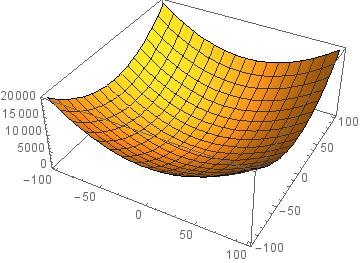
\includegraphics[scale = 0.3]{complexz2abssurface}
%    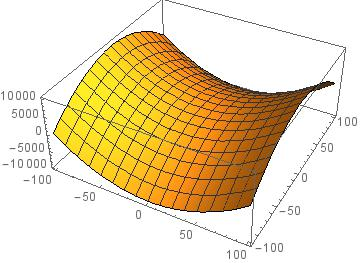
\includegraphics[scale = 0.3]{complexz2resurface}
%    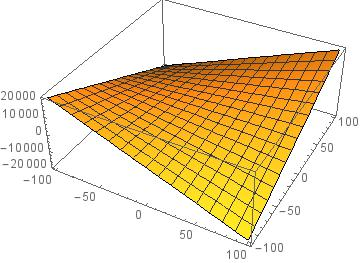
\includegraphics[scale = 0.3]{complexz2imsurface}

%    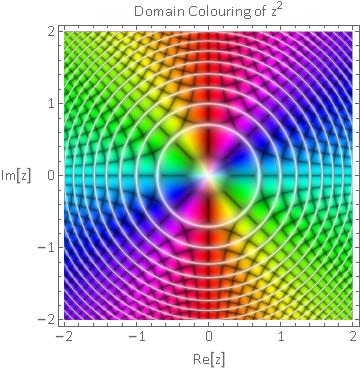
\includegraphics[scale = 0.5]{colorz2}
%    \end{center}
    %
%    The graph of the real part $w = \Re(z^2)$ can be written as $w = \Re(z)^2 - \Im(z)^2$. This is a hyperbololic paraboloid, as is the imaginary part can be written $w = 2\Re(z)\Im(z)$, with level curves
    %
%    \[ \Im(z) = \frac{w}{2 \Re(z)} \]
    %
%    Graphs of the three component functions are shown above.
%\end{example}
%
The standard definition of differentiability of real-valued functions generalizes easily to complex-valued functions, but the definition hides the fact that complex differentiability is a much stronger property than standard differentiability. A complex-valued function $f$ defined in a neighbourhood of a point $z$ = is {\bf complex differentiable}, {\bf holomorphic}, or {\bf regular} at $z$ if the limit
%
\[ f'(z) = \lim_{h \to 0} \frac{f(z + h) - f(z)}{h} \]
%
exists. Unlike differentiability on the real plane, we note that complex differentiability is a much stronger condition on the local behaviour of $f$ around $z$. Whereas the real-valued limit can only by approached by two directions, complex differentiability is a limit approached from any approach trajectory. The set of all holomorphic functions defined on a domain $D$ is denoted $C^\omega(D)$. If $f$ is complex differentiable at $z$, then the limit implies exactly that we can write $f(z + w) = f(z) + w f'(z) + o(w)$. In terms of complex multiplication, that means that $f$ is locally well approximated by a translation, combined with a rotation and a dilation. We leave it to verify that the addition, multiplication, quotient, and chain rule continue to hold from normal calculus, and the proofs are algebraically the same.

\begin{example}
    Every polynomial $f(z) = a_0 + a_1z + \dots + a_nz^n$ is differentiable at any point in the complex plane, with derivative $f'(z) = a_1 + 2a_2z + \dots + na_nz^{n-1}$. It is easy to see that the derivative of $w = z$ is $w' = 1$, and then the addition and product rule verifies the rule for all polynomials.
\end{example}

\begin{example}
    The function $w = 1/z$ is differentiable on $\mathbf{C} - \{ 0 \}$, because
    %
    \[ \lim_{h \to 0} \frac{(z + h)^{-1} - z^{-1}}{h} = \lim_{h \to 0} -\frac{1}{z(z+h)} = -\frac{1}{z^2} \]
    %
    Using the product rule, this implies that for $w = z^{-n}$, $w' = -nz^{-(n+1)}$.
\end{example}

\begin{example}
    The function $f(z) = \overline{z}$, though just a simple reflection in the complex plane, is not {\it complex} differentiable anywhere. This is because
    %
    \[ \lim_{h \to 0} \frac{\overline{z + h} - \overline{z}}{h} = \lim_{h \to 0} \frac{\overline{h}}{h} \]
    %
    And this limit does not exist, because if we approach the limit from the imaginary axis, with $h = ti$, then $\overline{h}/h = -1$, and if we approach the limit from the real axis, with $h = t$, then $\overline{h}/h = 1$. A reflection is not locally a rotation and a dilation.
\end{example}

\begin{theorem}
    If $f$ is holomorphic, and $\text{Re}(f)$, $\text{Im}(f)$, or $|f|$ is constant, then $f$ itself is constant.
\end{theorem}
\begin{proof}
    We have
    %
    \[ \frac{\partial f}{\partial \overline{z}} = \frac{\partial f}{\partial x} - i \frac{\partial f}{\partial y} = 0 \]
    %
    Since $\text{Re}(f)$ is constant, the partial derivative of this in any direction is zero. Thus
    %
    \[ \frac{\partial f}{\partial \overline{z}} = i \frac{\partial \text{Im} f}{\partial x} + \frac{\partial \text{Im}(f)}{\partial y} = 0 \]
    %
    Which implies the partial derivatives of $\text{Im}(f)$ vanish, so $\text{Im}(f)$ is constant. Similar results hold for $\text{Im}(f)$. If $|f|^2 = f \overline{f}$ is constant,
    %
    \[ 0 = \frac{\partial |f|^2}{\partial z} = \overline{f} f' \]
    %
    So whenever $f$ is nonzero, $f' = 0$, so $f$ is constant.
\end{proof}

We previously noted that complex multiplication corresponds to a rotation and a dilation. In particular, for each $w$, the map $T_w(z) = wz$ is a linear map from $\mathbf{C}$ to itself. Viewing $\mathbf{C}$ as $\mathbf{R}^2$, we see it has a matrix representation
%
\[ T_w = \begin{pmatrix} w_1 & w_2 \\ -w_2 & w_1 \end{pmatrix} \]
%
The function $f(z) = \overline{z}$, viewed as a function from $\mathbf{R}^2$ to $\mathbf{R}^2$, is certainly differentiable, and in fact, $C^\infty$. It is linear, with matrix representation
%
\[ \begin{pmatrix} +1 & 0 \\ 0 & -1 \end{pmatrix} \]
%
This cannot be put in the form $T_w$ for any $w$, which reflects the nonexistence of a complex derivative of the function. Not all linear endomorphisms of the plane are homotheties. However, there are relations which guarantee a linear map to be a rotation and a dilation. In fact, the matrix representation above shows that a function $f = u + iv$ is complex differentiable at a point if and only if it is real differentiable, and
%
\[ \frac{\partial u}{\partial x} = \frac{\partial v}{\partial y}\ \ \ \ \ \frac{\partial u}{\partial y} = -\frac{\partial v}{\partial x} \]
%
These are known as the {\bf Cauchy-Riemann equations}.

As an alternate viewpoint, we can also approach this purely from the complex perspective, something we will find often gives the most elegant arguments as we go deeper into complex analysis. If $f$ is complex differentiable at $z$, then
%
\[ f(z + w) = f(z) + f'(z)w + o(w) \]
%
so
%
\[ \frac{\partial f}{\partial x} = \lim_{t \to 0} \frac{f(z + t) - f(z)}{t} = \lim_{t \to 0} \frac{f'(z)t + o(t)}{t} = f'(z) \]
\[ \frac{\partial f}{\partial y} = \lim_{t \to 0} \frac{f(z + it) - f(z)}{t} = \lim_{t \to 0} \frac{itf'(z) + o(t)}{t} = if'(z) \]
%
If $f$ is complex differentiable, then we find
%
\[ \frac{\partial f}{\partial y} = i\frac{\partial f}{\partial x} \]
%
This is precisely the Cauchy Riemann equations in complex form. Often, the differential operators
%
\[ \frac{\partial}{\partial z} = \frac{\partial}{\partial x} - i \frac{\partial}{\partial y}\ \ \ \ \frac{\partial}{\partial \overline{z}} = \frac{\partial}{\partial x} + i \frac{\partial}{\partial y} \]
%
are written so that $f$ satisfies the Cauchy Riemann equations precisely when $\partial f/\partial \overline{z} = 0$. if $f$ is differentiable, the derivative rule can also be described by
%
\[ f(z_0 + z) = f(z_0) + z \frac{\partial f}{\partial z}(z_0) + \overline{z} \frac{\partial f}{\partial \overline{z}}(z_0) + o(|z|) \]
%
which is just another way of describing the standard derivative rule
%
\[ f(z_0 + z) = f(z_0) + (Df)(z_0)(z) + o(|z|) \]
%
Thus a differentiable function has a combination of a complex differentiable part, and a `conjugate differential' part.











\section{Power Series}

Polynomials are the simplest examples of holomorphic functions. Our next family of holomorphic functions will be obtained by taking limits of polynomials. In fact, we will soon show that this family essentially contains all holomorphic functions. A {\bf formal power series} about a point $z_0$ is an `infinite dimensional polynomial'
%
\[ \sum_{n = 0}^\infty c_n (z - z_0)^n \]
%
We may evaluate a power series to obtain a function $f$, defined as
%
\[ f(z) = \sum_{k = 0}^\infty a_k (z - z_0)^k \]
%
whose domain is the set where the series converges. A function $f$ can be {\bf expanded in a power series} at a point $z_0$ if we may write $f$ as a power series locally around $z_0$. An {\bf analytic} function is a function which can be locally expanded as a power series at every point in its domain.

Standard tricks from real power series come into play here, and the proofs go unedited. The most useful is the root test, or Cauchy-Hadamard theorem, which states that, if we define $1/R = \limsup_{n \to \infty} |c_n|^{1/n}$, then the power series $f$ converges locally uniformly for $|z - z_0| < R$, and diverges for $|z - z_0| > R$. It may sometimes be easier to apply the ratio test. If the limit $1/L = \lim_{n \to \infty} | c_{n+1}/c_n|$ exists, then $f$ converges for $|z - z_0| < L$, and diverges for $|z - z_0| > L$. These statements do not say anything about what happens on the boundary, when $|z - z_0|$ is equal to $R$ or $L$.

\begin{example}
    The most important power series, and perhaps the most important function in mathematics, is the exponential function, defined at all points in the complex plane by the formula
    %
    \[ e^z = \exp(z) = \sum_{n = 0}^\infty \frac{z^n}{n!} \]
    %
    Which converges for all $z$ by the ratio test. The product formula shows
    %
    \begin{align*}
    \exp(z + w) &= \sum_{k = 0}^\infty \frac{(z + w)^k}{k!} = \sum_{k = 0}^\infty \sum_{j = 0}^k \binom{k}{j} \frac{z^j w^{k-j}}{k!}\\
    &= \sum_{k = 0}^\infty \sum_{j = 0}^k \frac{z^j}{j!} \frac{w^{k-j}}{(k - j)!} = \exp(z) \exp(w)
    \end{align*}
    %
    which gives us the multiplicative property of the function.
\end{example}

\begin{example}
    The hypergeometric series is defined for $\alpha, \beta \in \mathbf{C}$, and a number $\gamma$ which is {\it not} a negative integer by the formula
    %
    \begin{align*}
        F(\alpha,\beta,\gamma;z) &= \sum_{n = 1}^\infty \frac{\alpha(\alpha+1)\dots(\alpha + n - 1) \beta(\beta + 1) \dots (\beta + n - 1)}{\gamma (\gamma + 1) \dots (\gamma + n - 1)} \frac{z^n}{n!}\\
        &= \sum_{n = 1}^\infty \frac{(\alpha)_n (\beta)_n}{(\gamma)_n} \frac{z^n}{n!}
    \end{align*}
    %
    The notation $(\cdot)_n$ is known as a Pockhammer symbol. We calculate that
    %
    \begin{align*}
        \log \left( \prod_{m = 0}^{N-1} (t + m) \right) &= \sum_{m = 0}^{N-1} \log(t + m) = \int_t^{t + N} \log x\; dx + O_t(\log N)\\
        &= N \log(t + N) - N + O_t(\log N)
    \end{align*}
    %
    In particular, $\log(N!) = N \log N - N + O(\log N)$. This means
    %
    \[ \log \left( \left( \frac{(\alpha)_N (\beta)_N}{(\lambda)_N} \frac{1}{N!} \right)^{1/N} \right) = \frac{O_{\lambda, \alpha,\beta}(\log N)}{N} = o_{\lambda, \alpha, \beta}(1) \]
    %
    so
    %
    \[ \left( \frac{(\alpha)_N (\beta)_N}{(\lambda)_N} \frac{1}{N!} \right)^{1/N} \to 1 \]
    %
    which implies the series has a radius of convergence of one.
\end{example}

\begin{example}
    If we define the Bessel function
    %
    \[ J_m(z) = (z/2)^m \sum_{n = 0}^\infty \frac{(-1)^n}{n! (n+m)!} (z/2)^{2n} \]
    %
    Then we calculate
    %
    \begin{align*}
        \log \left( \left( \frac{1}{2^{2n} n! (n+m)!} \right)^{1/n} \right) &=  \frac{-n \log n + O_t(n)}{2n} \to -\infty
    \end{align*}
    %
    so $J_m$ is defined by a power series everywhere.
\end{example}

Calculus tells us that the derivative of the exponential function is the exponential function itself. If there is any justice in the world, this idea should extend to the complex case. We can formally calculate
%
\[ \exp'(z) = \sum_{n = 0}^\infty \left( \frac{z^n}{n!} \right)' = \sum_{n = 1}^\infty \frac{z^{n-1}}{(n-1)!} = \sum_{n = 0}^\infty \frac{z^n}{n!} = \exp(z) \]
%
But how do we know that the derivative of the power series can be obtained by differentiating each term in the series?

\begin{theorem}
    Let
    %
    \[ f(z) = \sum_{n = 0}^\infty a_n z^n \]
    %
    be a power series, convergent inside a disk $D$. Then $f$ is holomorphic in $D$, and
    %
    \[ f'(z) = \sum_{n = 1}^\infty n a_n z^{n-1} \]
\end{theorem}
\begin{proof}
    The fact that the power series defining $f'$ converges in $D$ follows from the Hadamard formula. Now let us verify that this series, which defines a function $g$, approaches the derivative of $f$. Define $S_n$ to be the finite polynomial of degree $n$ defined by $f$, $S_n(z) = \sum_{k = 0}^n a_k z^k$. Let $E_n$ denote the error term, $E_n(z) = \sum_{k = n+1}^\infty a_k z^k$. Then $S_n'(z) = \sum_{k = 1}^n k a_k z^{k-1}$, and
    %
    \[ \frac{f(z + w) - f(z)}{w} = \left[ \frac{S_n(z + w) - S_n(z)}{w} - S_n'(z) \right] + \left[ \frac{E_n(z + w) - E_n(z)}{w} \right] + S_n'(z) \]
    %
    The first term converges to zero for small enough $w$. The third term converges to $g(z)$ as $n \to \infty$. The only tricky component is the second term. Since $a^n - b^n = (a - b)(a^{n-1} + a^{n-2}b + \dots + ab^{n-2} + b^{n-1})$. If we choose $|z|, |z + w| < r - \varepsilon$, then
    %
    \begin{align*}
        \left| \frac{E_n(z + w) - E_n(z)}{w} \right| &= \left| \sum_{k = n + 1}^\infty a_k \frac{(z + w)^k - z^k}{w} \right| \leq \sum_{k = n + 1}^\infty k |a_k| (r - \varepsilon)^{n-1}
    \end{align*}
    %
    The right side is a convergent power series, and hence as $n \to \infty$, the term converges to zero. By picking $n$ large enough, and $|z - w|$ small enough, the value can be made as close to $g$ as possible.
\end{proof}

\begin{corollary}
    The power series $f$ is infinitely differentiable in $D$, with
    %
    \[ f^{(m)}(z) = \sum_{n = m}^\infty \frac{n!}{(n - m)!} a_n z^{n-m} \]
\end{corollary}
\begin{proof}
    All that remains to be proven is that $f'$ has the same radius of convergence as $f$, so that we may successively apply the theorem. If $f$ has radius of converge $R$, then $R^{-1} = \limsup |a_n|^{1/n}$, and so
    %
    \[ \limsup |a_n|^{1/n} n^{1/n} = \lim n^{1/n} \limsup |a_n|^{1/n} = \limsup |a_n|^{1/n} \]
    %
    and so $f'$ has the same radius of convergence as $f$.
\end{proof}

\begin{corollary}
    Every analytic function is holomorphic on it's domain's interior.
\end{corollary}











\section{Integration Along Curves}

One distinguishing feature separating the study of complex analysis from Newton's one dimensional calculus is the reliance on line integration, which you may have encountered in multivariate calculus. Firstly, we will find ourselves not integrating over the whole complex plane, but instead integrating over curves lying in the complex plane. A {\bf smooth curve} is an immersion of a closed interval into $\mathbf{C}$ (viewing the interval as an oriented one dimensional manifold with boundary, and $\mathbf{C}$ as a two dimensional manifold). More simply, we define a {\bf smooth parameterization} $z: [a,b] \to \mathbf{C}$ to be a differentiable map whose derivative is continuous, and $z'(t) \neq 0$ for all $t \in [a,b]$, where we interpret $z'(a)$ and $z'(b)$ as the left and right hand limits
%
\[ \lim_{h \to 0^+} \frac{z(a + h) - z(a)}{h}\ \ \ \ \ \lim_{h \to 0^-} \frac{z(b + h) - z(b)}{h} \]
%
Two smooth curves $z_0: [a_0,b_0] \to \mathbf{C}$ and $z_1: [a_1,b_1] \to \mathbf{C}$ are {\bf equivalent} if there is a continuously differentiable function $s: [a_0,b_0] \to [a_1,b_1]$ with $s'(t) > 0$ for all $t$, such that $z_0(t) = z_1(s(t))$ for all $t \in [a_0,b_0]$. We then define a smooth curve to be an equivalence class of smooth parameterizations. More generally, a {\bf piecewise smooth curve} is an equivalence class of continuous parameterizations $z: [a,b] \to \mathbf{C}$, with values $a = a_0 < a_1 < \dots < a_n = b$ such that $z$ is a smooth curve on $[a_i,a_{i+1}]$, where $z_0: [a_0,b_0] \to \mathbf{C}$ and $z_1:[c_0,d_0] \to \mathbf{C}$ are equivalent if there are $a = a_0 < \dots < a_n = b$ and $c = c_0 < \dots < b_n = d$ such that $z_0$ and $z_1$ are equivalent on each of the intervals $[a_i,a_{i+1}]$ and $[c_i,c_{i+1}]$. We rarely need to discuss classes of curves more general than this in complex analysis, and certainly not in elementary complex analysis.

\begin{example}
    The standard example of a curve is the circle $C_r(z_0)$, of radius $r$ centered at $z_0$. The {\it positive orientation} of this curve is given by the parameterization $z(t) = z_0 + re^{it}$ on $[0,2\pi]$, and the {\it negative orientation} $z(t) = z_0 + re^{-it}$, also defined on $[0,2\pi]$. In general, we will interpret $C_r(z_0)$ as having the positive orientation.
\end{example}

We will also need to introduce slightly more terminology to manipulate curves. The {\bf trace} of a curve $C$ is the point set corresponding to the curve. It is the image of all the parameterizations of the curve. The {\bf inverse orientation} of a curve with parameterization $z: [a,b] \to \mathbf{C}$, which is the curve with parameterization $z^-: [a,b] \to \mathbf{C}$ with $z^-(t) = z(a+b-t)$. A curve $z: [a,b] \to \mathbf{C}$ is {\bf closed} if $z(a) = z(b)$, which means its image forms a `closed loop' in the plane. Now given a smooth curve $C$ with parameterization $z: [a,b] \to \mathbf{C}$, and a continuous function defined on the trace of $C$, we define the {\bf line integral} of $f$ on $C$ as
%
\[ \int_C f(z) dz = \int_a^b f(z(t)) z'(t) dt \]
%
which we can remember by the mneumonic
%
\[ f(z) dz = f(z) \left( \frac{dz}{dt} \right) dt \]
%
so we can obtain the formula by `multiplying by a $dt/dt$ factor'. If $z'$ is only piecewise smooth, with partition $a_0 < \dots < a_n$, then we define
%
\[ \int_C f(z) dz = \sum \int_{a_i}^{a_{i+1}} f(z(t)) z'(t) dt \]
%
The change of variables formula for one dimensional integrals verifies that these definitions are independent of parameterization.

\begin{theorem}
    The line integral satisfies the following properties
    %
    \begin{itemize}
        \item For a given curve $C$ on some domain $D$, for any two $f,g \in C(D)$, $\alpha, \beta \in \mathbf{C}$,
        %
        \[ \int_C (\alpha f + \beta g)(z) dz = \alpha \int_C f(z) dz + \beta \int_C g(z) dz \]

        \item If $C^-$ is the reverse orientation of $C$, then
        %
        \[ \int_{C^-} f(z) dz = - \int_C f(z) dz \]

        \item One has
        %
        \[ \left| \int_C f(z) dz \right| \leq l(C) \| f \|_\infty \]
        %
        where $\| f \|_\infty$ is the supremum of $f$ over image of the curve $C$, and $l(C)$ is the {\bf length} of the curve $C$, defined to be the integral $\int_a^b |z'(t)| dt$.
    \end{itemize}
\end{theorem}
\begin{proof}
    The first theorem follows by the linearity of one dimensional integration by expanding out formulas, and the second theorem follows because $(z^-)'(t) = -z'(a+b-t)$. Finally, the third theorem follows because if $z: [a,b] \to \mathbf{C}$ is smooth, then
    %
    \[ \left| \int_C f(z)dz \right| = \left| \int_a^b f(z(t)) z'(t) dt \right| \leq \int_a^b |f(z(t))||z'(t)| dt \leq \| f \|_\infty \int_a^b |z'(t)| dt \]
    %
    and the result for piecewise smooth curves follows by linearity.
\end{proof}

Finally in our review of line integration, we recall a very useful result. We say a function $f: D \to \mathbf{C}$ on some domain $D$ has a {\bf primitive} if there is a function $F: D \to \mathbf{C}$ holomorphic on $D$ such that $F'(z) = f(z)$.

\begin{theorem}
    If $f$ is continuous, and has a primitive $F$, then a curve $C$ begining at $z_0$ and ending at $z_1$ has
    %
    \[ \int_C f(z)dz = F(z_1) - F(z_0) \]
    %
    In particular, if $C$ is a closed curve, then $\int_C f(z)dz = 0$.
\end{theorem}
\begin{proof}
    If $C$ is smooth, then
    %
    \[ \int_C f(z)dz = \int_a^b f(z(t)) z'(t) dt \]
    %
    Now if $F'(z) = f(z)$ for each $z \in D$, then the chain rule (which is easily proved for compositions of functions from intervals to $\mathbf{C}$ and from holomorphic functions on $\mathbf{C}$) implies that $(F \circ z)'(t) = F'(z(t)) z'(t)$, and therefore the fundamental theorem of calculus (applied componentwise on the integral of the complex valued function $f(z(t)) z'(t)$), we conclude that
    %
    \[ \int_a^b f(z(t)) z'(t) dt = F(z(b)) - F(z(a)) = F(w) - F(z) \]
    %
    The theorem is then proved for piecewise smooth curves by applying this theorem for the individual smooth curves and then applying a telescoping summation.
\end{proof}

\begin{corollary}
    If $f$ is holomorphic, with $f' = 0$, then $f$ is constant on $D$.
\end{corollary}
\begin{proof}
    If $z_0$ and $z_1$ are two points, let $C$ be a smooth curve beginning at $z_0$ and ending at $z_1$. Then since $f' = 0$, $\int_C f'(z) dz = 0$. But also since $f'$ has a primitive $f$, we find that
    %
    \[ \int_C f'(z) dz = f(z_1) - f(z_0) \]
    %
    and hence $f(z_0) = f(z_1)$.
\end{proof}

\begin{example}
    The function $f(z) = 1/z$ does not have a primitive in $\mathbf{C} - \{ 0 \}$, where it is defined, because
    %
    \[ \int_{S^1} \frac{dz}{z} = \int_0^{2\pi} \frac{ie^{it}}{e^{it}} = \int_0^{2\pi} i = 2 \pi i \]
    %
    If $1/z$ did have a primitive, we would conclude this integral is zero. We shall find that this is the essential holomorphic function without a primitive, and we will use this integral to calculate a great many functions.
\end{example}

We know that if $f$ has a primitive $F$, then the integral of $f$ vanishes over all closed curves $\gamma$. But conversely, if the integral of a continuous $f$ over all closed curves vanishes, then such a primitive exists. The idea is to fix a point $z_0$ in the domain, and to define $F(z_1) = \int_\gamma f(z)\; dz$, where $\gamma$ is a curve from $z_0$ to $z_1$. We find that
%
\[ \frac{\partial F}{\partial x} = f(z)\ \ \ \ \ \frac{\partial F}{\partial y} = i f(z) \]
%
follows from the fundamental theorem of calculus. But this implies that $F$ is holomorphic by the Cauchy Riemann equations, and the fact that $f$ is continuous.







\section{Harmonic Functions}

A function $f: \mathbf{R}^2 \to \mathbf{C}$ is known as harmonic if
%
\[ \Delta f = \frac{\partial^2 f}{\partial x^2} + \frac{\partial^2 f}{\partial y^2} = 0 \]
%
We now discuss a connection which allows us to reduce their study to the study of holomorphic functions. We calculate
%
\[ \partial_z \partial_{\overline{z}} = \frac{(\partial_x - i \partial_y)(\partial_x + i \partial_y)}{4} = \frac{\partial^2_x + i \partial_x \partial_y - i \partial_y \partial_x + \partial_y^2}{4} = \frac{\Delta}{4} \]
%
Thus any holomorphic or antiholomorphic function is harmonic, as is it's real and imaginary part. Conversely, suppose that $g$ is a real-valued harmonic function. Then $\partial_{\overline{z}} \partial_z g = 0$, so $\partial_z g$ is holomorphic. We will later find that any holomorphic locally has an antiderivative, so in particular, we can find a holomorphic function $f$ with $f' = 2 \partial_z g$. But this means that if $f_0$ is the real part of $f$,
%
\[ \partial_x f_0 - i \partial_y f_0 = f' = 2 \partial_z g = \partial_x g - i \partial_y g \]
%
so $\nabla f_0 = \nabla g$, implying $f_0$ and $g$ differ by a constant. Patching the $f_0$ together on the domain of $g$ shows that $g$ is the real part of a holomorphic function. In particular, applying the Cauchy integral formula on $C_r(z_0)$ means
%
\[ f(z_0) = \frac{1}{2 \pi i} \int_{C_r(z_0)} \frac{f(z)}{z - z_0}\; dz = \frac{1}{2\pi} \int_0^{2\pi} f(z_0 + r e^{it})\; dt  \]
%
Taking the real parts on both sides gives
%
\[ g(z_0) = \frac{1}{2\pi} \int_0^{2\pi} f(z_0 + e^{it})\; dt \]
%
So any harmonic function satisfies the mean value formula; the average value of the function around a circle is the same as the value of that function at the centre of the circle. Note that this is not necessarily true for the average of the function over every curve, since in the calculations above for curves other than circles the imaginary parts of $f$ might contribute to the imaginary part of the integral.







\chapter{Cauchy's Theorem}

Cauchy's theorem says that the integral of a holomorphic function about a closed curve is always zero. This is simple, but forms the backbone for the theory of holomorphic functions. Originally, certain regularity were assumed on holomorphic functions to obtain Cauchy's theorem. But it was later discovered that one can obtain Cauchy's theorem assuming only that the function is holomorphic at each point in the region, and it is this procedure we will use to show the regularity of holomorphic functions completely.

\begin{theorem}[Goursat's lemma]
    If $T$ is a triangle, and $f$ is holomorphic in an open set containing the triangle and it's interior, then
    %
    \[ \int_T f(z)\; dz = 0 \]
\end{theorem}
\begin{proof}
    We can split the triangle $T$ into four smaller triangles $A$, $B$, $C$, and $D$, each with half the diameter and length. Since
    %
    \[ \int_T f(z)\; dz = \left( \int_{A} f(z)\; dz + \int_B f(z)\; dz + \int_C f(z)\; dz + \int_D f(z)\; dz \right) \]
    %
    We may choose one such triangle $T_1$ with
    %
    \[ \left| \int_{T_1} f(z)\; dz \right| \geq \left| \int_T f(z)\; dz \right| \]
    %
    Continuing inductively, we can find a nested family of rectangles $T_1 \supset T_2 \supset \dots T_n$ with $\text{diam}(T_n) = \text{diam}(T)/2^n$, $l(T_n) = l(T)/2^n$, and
    %
    \[ \left| \int_{T_n} f(z)\; dz \right| \geq 4^{-n} \left| \int_T f(z)\; dz \right| \]
    %
    As $n \to \infty$, $\text{diam}(T_n) \to 0$, so $\bigcap T_n$ contains a unique point $z_0$. We can write $f(z) = f(z_0) + f'(z_0) (z - z_0) + \psi(z - z_0)(z - z_0)$, with $\psi(w) \to 0$ as $w \to 0$. Now it is easy to calculate that
    %
    \[ \int_{T_n} f(z_0)\; dz = f'(z_0) \int_{T_n} (z - z_0)\; dz = 0 \]
    %
    so if $|\psi(z - z_0)| \leq \varepsilon$ for $z$ lying on $T_n$,
    %
    \begin{align*}
        \left| \int_T f(z)\; dz \right| \leq 4^n \left| \int_{T_n} f(z)\; dz \right| &= 4^n \left| \int_{T_n} \psi(z-z_0)(z - z_0)\; dz \right|\\
        &\leq 4^n \varepsilon l(T_n) \text{diam}(T_n) = \varepsilon l(T) \text{diam}(T)
    \end{align*}
    %
    and thus as $n \to \infty$, we can take $\varepsilon \to 0$ to conclude the integral over the triangle is zero.
\end{proof}

\begin{remark}
    Note that the proof of this theorem remains true if we replace the condition that $f$ is holomorphic in $D$ with the weaker condition that $f$ is analytic except at finitely many points $z_1, \dots, z_N$ in the interior of the triangle, with the property that $\lim_{z \to z_n} (z - z_n) f(z) = 0$ for each $n$. By splitting our triangles into smaller triangles, we may assume that there is only a single point with this property in the triangle. By splitting our triangle into smaller triangles, and applying the theorem above in all regions but the region containing the triangle, we determine that the integral over the entire region is equal to the integral of $f$ about an equilateral triangle $T'$ centered at $z$, of arbitrarily small length. But if $T'$ is small enough that $|z - z_n| |f(z)| \leq \varepsilon$ for $z$ on $T'$, then
    %
    \[ \left| \int_{T'} f(z)\; dz \right| \leq \varepsilon \left| \int_{T'} \frac{dz}{z - z_n} \right| \]
    %
    and one verifies that
    %
    \[ \left| \int_{T'} \frac{dz}{z - z_n} \right| \lesssim 1 \]
    %
    since the distance from points on the triangle to $z_n$ is proportional to the perimeter of the triangle. This concludes the argument.
\end{remark}

Attaching two triangles together, we can obtain Cauchy's theorem for a rectangle. Given a holomorphic function $f$ on a circle, by defining $F(w)$ to be the line integral from the centre of the circle to $w$ on either half of the rectangle parallel to the axis, well defined by Goursat's lemma, we find a function $F$ with $F' = f$, so $f$ has a primitive, and so Cauchy's theorem holds in a circle. More generally, this holds under the weaker condition where $f$ is defined except at finitely many interior points $z_1, \dots, z_N$ with $\lim (z - z_n) f(z) = 0$, because we can with a few edge cases not included in the previous case find a function $F$ with $F' = f$.

\begin{lemma}
    If $\gamma$ is a closed curve not passing through $z_0$, then
    %
    \[ \eta(\gamma,z_0) = \frac{1}{2 \pi i} \int_\gamma \frac{dz}{z - z_0} \]
    %
    is an integer, known as the {\bf winding number} of $\gamma$ around $z_0$.
\end{lemma}
\begin{proof}
    If we parameterize $\gamma$ by $z$, then consider the continuous function
    %
    \[ h(t) = \int_a^t \frac{z'(t)}{z(t) - z_0}\; dt \]
    %
    And we have $h'(t) = z'(t)/(z(t) - z_0)$. Thus the derivative of $g(t) = e^{-h(t)}(z(t) - z_0)$ vanishes, so $g(t)$ must be constant, so
    %
    \[ e^{h(t)} = \frac{z(t) - z_0}{z(a) - z_0} \]
    %
    In particular,
    %
    \[ e^{h(b)} = \frac{z(b) - z_0}{z(a) - z_0} = 1 \]
    %
    so $h(b)$ must be a multiple of $2 \pi i$, completing the proof.
\end{proof}

Cauchy's theorem implies that if $\gamma$ is contained in a circle, and $z_0$ is a point lying outside of the circle, then $\eta(\gamma,z_0) = 0$. Furthermore, if there is a curve between two points $z_0$ and $z_1$ not passing through $\gamma$, then $\eta(\gamma,z_0) = \eta(\gamma,z_1)$. Since we can replace the curve with a polygon, it suffices to prove this assuming the curve is a line segment. Outside of the segment the function $(z - z_0)(z - z_1)^{-1}$ is never a negative number, so $\log((z-z_0)/(z-z_1))$ is analytic in the complement of the segment, and it's derivative is $(z - z_0)^{-1} - (z - z_1)^{-1}$, hence Cauchy's theorem implies that
%
\[ \int_\gamma \frac{dz}{z - z_0} = \int_\gamma \frac{dz}{z - z_1} \]
%
hence $\eta(\gamma,z_0) = \eta(\gamma,z_1)$.

\begin{theorem}
    If $f$ is holomorphic in a disc $D$ containing a point $w$, and $\gamma$ is a closed curve in $D$ not passing through $w$, then
    %
    \[ \int_\gamma \frac{f(z)}{z - w} = 2 \pi i \eta(\gamma,w) f(w) \]
\end{theorem}
\begin{proof}
    Since $g(z) = (f(z) - f(w))/(z-w)$ is holomorphic everywhere in $D$ except at $w$, and $\lim_{z \to w} (z - w) g(z) = 0$, we can apply our remark to conclude that
    %
    \[ \int_\gamma \frac{f(z)}{z - w}\; dz = \int_\gamma \frac{f(w)}{z - w}\; dz = 2 \pi i \eta(\gamma,w) f(w) \]
    %
    Thus the theorem becomes an explicit calculation.
\end{proof}

\begin{remark}
Integral representation formulas are very important in analysis, because they enable us to control a function from its behaviour on a very small set, and also use it to show the function is suitably regular.
\end{remark}

\section{Consequences of Cauchy's Formula}

A simple corollary of Cauchy's integral formula, proved by induction, shows any holomorphic function is completely smooth.

\begin{theorem}
    If $f$ is holomorphic, then $f$ has derivatives of all orders, with
    %
    \[ f^{(n)}(w) = \frac{n!}{2 \pi i \eta(\gamma,w)} \int_\gamma \frac{f(z)}{(z - w)^{n+1}}\; dz \]
    %
    where $\gamma$ is some closed curve with nonzero winding number obout $w$.
\end{theorem}
\begin{proof}
    To prove this, it would suffice to reduce the question to the theory of differentiation under the integral sign in real variable theory. But there is a more elementary proof. We know this is true for $n = 0$. And now by induction, if it is true for $n$, then
    %
    \begin{align*}
        \frac{n!}{2 \pi i \eta(\gamma,w)} \int_\gamma & \left( \frac{f(z)}{(z - w)^{n+1}} - \frac{f(z)}{(z - w_0)^{n+1}} \right)\; dz\\
        &= \frac{n!}{2 \pi i \eta(\gamma,w)} \int_\gamma \frac{f(z)}{w_0 - w} \left( \frac{1}{z - w} - \frac{1}{z - w_0} \right) \left( \sum_{k = 0}^n \frac{1}{(z - w)^{n-k}(z - w_0)^k} \right)\\
        &= \frac{n!}{2 \pi i \eta(\gamma,w)} \int_\gamma \frac{f(z)}{(z - w)(z - w_0)} \left( \sum_{k = 0}^n \frac{1}{(z - w)^{n-k}(z - w_0)^k} \right)
    \end{align*}
    %
    and as $w \to w_0$, we conclude that
    %
    \[ f^{(n+1)}(w_0) = \frac{(n+1)!}{2 \pi i \eta(\gamma,w)} \int_\gamma \frac{f(z)}{(z - w_0)^{n+2}}\; dz \]
    %
    which completes the proof.
\end{proof}

\begin{remark}
    Because of this, we obtain that for each $z$ upon which $f$ is holomorphic,
    %
    \[ | f^{(n)}(z) | \leq \frac{1}{\eta(\gamma,z)} \frac{n!}{2\pi} \frac{\| f \|_{L^\infty(\gamma)}}{d(z,\gamma)^n} l(\gamma) \]
    %
    a result known as Cauchy's inequality. In the case that $\gamma$ is just a disk centered at $z$ with radius $R$, the formula simplifies to
    %
    \[ | f^{(n)}(z) | \leq \frac{n! \| f \|_{L^\infty(\gamma)}}{R^n} \]
    %
    So bounding $f$ on a circle bounds the derivatives on the interior of the circle.
\end{remark}

\begin{corollary}
    If $f: D \to D$ is holomorphic, with $f(z_0) = z_0$ and $f'(z_0) = 1$, then $f$ is the identity function.
\end{corollary}
\begin{proof}
    Let $f^N = f \circ \dots \circ f$. If $f(z_0 + z) = z_0 + z + az^n + O(z^{n+1})$ for $z$ in a small neighbourhood of $z_0$, then $f^N(z_0 + z) = z_0 + z + Naz^n + O(z^{n+1})$. And by the Cauchy inequalities we obtain that if $B_R(z_0) \subset D \subset B_M(0)$,
    %
    \[ n! Na = (f^N)^{(n)}(z_0) \leq \frac{n! M}{R^n} \]
    %
    Thus $a = O(1/N)$, so as $N \to \infty$, we get $a = 0$, so $f(z_0 + z) = z_0 + z$.
\end{proof}

We have proved that if $f$ is continuous, and satisfies the Cauchy Riemann equations everywhere, then $f$ has smooth derivatives of all orders. If $f$ were $C^1$, then Cauchy's theorem would be very simple to prove as a consequence of Green's theorem. This is because if $f = u + iv$,
%
\[ \int_\gamma f(z)\; dz = \int_\gamma (u dx - v dy) + i \int_\gamma (u dy + v dx) \]
%
If $f$ is holomorphic in a simply connected domain $D$, and $\gamma$ is a closed curve, there exists a 2-chain $U$ in $D$ such that $\gamma = \partial U$, and so Green's theorem implies
%
\[ \int_\gamma f(z)\; dz = \int_U \frac{\partial u}{\partial y} + \frac{\partial v}{\partial x} + i \int_U \frac{\partial u}{\partial x} - \frac{\partial v}{\partial y} \]
%
Since $f$ is holomorphic, the Cauchy Riemann equations insure that both integrals above vanish, so that $\int_\gamma f(z)\; dz$. Thus using the $C^1$ properties of $f$, which we now can ensure even if $f$ is only continuous but holomorphic, the Cauchy theorem is generalized to the integral of any exact chain $\gamma$.

\begin{theorem}
    Any holomorphic function on a simply connected domain has a primitive.
\end{theorem}
\begin{proof}
    By taking a homotopy, we find $\int_\gamma f(z)\; dz$ depends only on the start and endpoints of $f$. Thus if we let $F(z) = \int_\gamma f(z)\; dz$, where $\gamma$ ends at $z$ and starts at $z_0$, then $F'(z) = f(z)$.
\end{proof}

\begin{theorem}
    Every holomorphic function is analytic.
\end{theorem}
\begin{proof}
    We calculate
%
\begin{align*}
    \frac{1}{z - w} &= \frac{1}{(z - z_0 - (w - z_0))} = \frac{1}{z - z_0} \frac{1}{1 - \frac{w - z_0}{z - z_0}}\\
    &= \frac{1}{z - z_0} \sum_{n = 0}^\infty \frac{(w - z_0)^n}{(z - z_0)^n}
\end{align*}
%
This converges uniformly when $|w - z_0| < |z - z_0|$. Thus if $f$ is holomorphic on an open domain containing a closed disk $D$, then
%
\begin{align*}
    f(w) &= \frac{1}{2 \pi i} \int_{\partial D} \frac{f(z)}{z - w}\; dz = \frac{1}{2 \pi i} \int_{\partial D} \sum_{n = 0}^\infty f(z) \frac{(w - z_0)^n}{(z - z_0)^{n+1}}\; dz\\
    &= \sum_{n = 0}^\infty \left( \frac{1}{2 \pi i} \int_{\partial D} \frac{f(z)}{(z - z_0)^{n+1}}\; dz \right) (w - z_0)^n\\
    &= \sum_{n = 0}^\infty \frac{f^{(n)}(z_0)}{n!} (w - z_0)^n
\end{align*}
%
Thus we obtain a power series expansion for $f(w)$ on the disk upon which it is defined. It is exactly the expansion you would expect by Cauchy's integral formula.
\end{proof}

An {\bf entire} function is a holomorphic function defined on the entire complex plane.

\begin{theorem}[Louville]
    Every bounded and entire function is constant.
\end{theorem}
\begin{proof}
    Consider Cauchy's inequality for $n = 1$, which we just proved. As we take the radius of the disc $D$ to $\infty$, the term $\| f \|_{L^\infty(\partial D)}$ remains bounded, so the numerator is bounded, whereas the denominator tends to $\infty$ for every $z$. Thus we conclude $f' = 0$, so $f$ is constant.
\end{proof}

\begin{theorem}[The Fundamental Theorem of Algebra]
    Every nonconstant polynomial over the complex numbers has a root.
\end{theorem}
\begin{proof}
    Let $f$ be a polynomial with no root over the complex numbers. If $f$ has degree $n$, then for large $z$, $f(z) = (1 + o(1))z^n$. Thus $1/f(z)$ is an entire function, and it is also bounded, since $|z|^n \lesssim |f(z)|$ for large $n$. Thus $1/f(z)$ is constant, so $f$ is constant.
\end{proof}

\begin{theorem}[Morera]
    If $f$ is a function with $\int_T f(z)\; dz = 0$ for all triangles $T$ in a region, then $f$ is holomorphic.
\end{theorem}
\begin{proof}
    Then we know there is a primitive function $F$ with $F' = f$. But $F$ is holomorphic, hence infinitely differentiable, and so $f$ must also be infinitely differentiable.
\end{proof}

Similar properties hold if we consider all affine copies of a simple piecewise smooth curve whose interior is simply connected.

\section{Sequences of Holomorphic Functions}

\begin{theorem}
    If a sequence $f_n$ of holomorphic functions converges locally uniformly to a holomorphic function $f$, then $f$ is holomorphic.
\end{theorem}
\begin{proof}
    Then for any triangle $T$, $f_n$ converges to $f$ uniformly on $T$, so
    %
    \[ \int_T f(z)\; dz = \lim \int_T f_n(z)\; dz = 0 \]
    %
    and so by Morera's theorem, $f$ is holomorphic.
\end{proof}

Note that if $f_n$ converge locally uniformly to $f$, then $f_n^{(m)}$ also converges locally uniformly to $f^{(m)}$ by the Cauchy inequality. A simple consequence is that if $\sum f_n$ converges locally uniformly, then the limit is holomorphic. Taking limits of this proposition leads to the fact that an integral of a continuous family of holomorphic functions is holmomorphic.

\begin{theorem}
    If $f(z,s)$ is continuous, and holomorphic in $z$ for each $s$, then we obtain a holomorphic function
    %
    \[ F(z) = \int_0^1 f(z,s)\; ds \]
\end{theorem}
\begin{proof}
    Using Morera's theorem, if $T$ is a triangle, then we can interchange integration to conclude that
    %
    \[ \int_T \int_0^1 f(z,s)\; ds\; dz = \int_0^1 \int_T f(z,s)\; dz\; ds = \int_0^1 0 = 0 \]
    %
    so the integral is holomorphic. Alternatively, $F$ is the uniform limit of Riemann sums, which are holomorphic.
\end{proof}

Now we discuss Runge's theorem, which tells us how well we can approximate harmonic functions on a domain by polynomials.

\begin{theorem}[Runge]
    Every holomorphic function defined in a neighbourhood of a compact set $K$ can be uniformly approximated by rational functions with poles in $K^c$. If $K^c$ is connected, then every such function can be uniformly approximated by polynomials.
\end{theorem}
\begin{proof}
    First we find a curve $\gamma$ in $K^c$ such that for any $w \in K$ and $f$ holomorphic on $K$,
    %
    \[ f(w) = \int_\gamma \frac{f(z)}{z - w} \]
    %
    It therefore suffices to approximate $f$ by rational functions on a very small set, the region encompassed by $\gamma$. If we parameterize, writing
    %
    \[ \int_\gamma \frac{f(z)}{z - w} = \int_a^b \frac{f(\gamma(t))}{\gamma(t) - w} \]
    %
    then this can be uniformly approximated on $K$ by Riemann sums, and each Riemann sum is a rational function.

    To show that on a connected $K^c$ we can approximate by polynomials, it suffices to approximate a function of the form $(z - w)^{-1}$, for $z \in K^c$, by a polynomial in $w$. If all points in $K$ have modulus bounded by $R$, and if $|z| > R$, then this is easy, for
    %
    \[ \frac{1}{z - w} = \sum_{k = 0}^\infty z^n/w^{n+1} \]
    %
    and this sum converges uniformly on the ball of radius $R$. If $|z| < R$, we form a path $\gamma$ connecting $z$ to a point $z_0$ we $|z_0| > R$. If $|w_0 - w_1| < d(K,\gamma)/2$, then
    %
    \[ \frac{1}{z - w_0} = \frac{1}{(z - w_1) - (z - w_0)} = \sum \frac{(z - w_0)^n}{(z - w_1)^{n+1}} \]
    %
    Thus if $(z - w_1)^{-1}$ can be approximated by polynomials, so too can $(z - w_0)^{-1}$. But if we now take a sequence of points along $\gamma$ at a distance $d(K,\gamma)/2$ apart from one another, we can successively approximate each inverse function by polynomials in the inverse function of the next point. Eventually, this gives us the approximation of $(z - w)^{-1}$ as polynomials in $(z_0 - w)^{-1}$, and this can be approximated by polynomials in $w$.
\end{proof}

\section{Uniqueness of Holomorphic Functions}

\begin{theorem}
    Let $f$ be holomorphic, such that the set of zeroes has a limit point $w$. Then $f = 0$ everywhere.
\end{theorem}
\begin{proof}
    Without loss of generality, assume $w = 0$. Write $f(z) = \sum_{n = 0}^\infty a_n z^n$ for $z$ close enough to zero. By continuity, $f(0) = a_0 = 0$. If $N > 0$ is the first index with $a_N \neq 0$, then
    %
    \[ f(z) = a_N z^N(1 + g(z)) \]
    %
    where $g$ is analytic in a neighbourhood of the origin, and $g(z) \to 0$ as $z \to 0$. But this means $f$ cannot have any zeroes in a neighbourhood of the origin, except for the origin itself. So all coefficients of the power series must vanish, so $f = 0$ uniformly.
\end{proof}

Thus if $f$ and $g$ are two holomorphic functions agreeing on an open set, or even on a countable set with a convergent point, then $f = g$ everywhere. Thus the values of a function on an arbitrarily small set determine the function uniquely, everywhere on its domain!

\begin{example}
    From Fourier analysis, we know the function $e^{-\pi x^2}$ is it's own Fourier transform. Thus for each real $\xi$ we have the integral equation
    %
    \[ e^{- \pi \xi^2} = \int_{-\infty}^\infty e^{- \pi x^2 - 2 \pi i \xi x}\; dx \]
    %
    Since both sides can be interpreted as holomorphic functions in the variable $\xi$, if $\xi$ is allowed to be complex, we conclude this integral formula holds for any complex $\xi$, not just the real $\xi$ which were used for the Fourier transform.
\end{example}

\section{The Reflection Principle}

Let $D$ be a region symmetric under conjugation, so $\overline{D} = D$. Split the region into it's upper and lower parts $D^+$ and $D^-$. We now discuss if it's possible to patch together two functions defined on either side of the half plane.

\begin{theorem}
    If $f^+$ and $f^-$ are functions defined on $D^+$ and $D^-$ respectively, and they can be extended to continuous functions extended to be defined on $D \cap \mathbf{R}$ in addition to their original domain, then this extension, when $f^+$ and $f^-$ are combined to form a function $f$, is holomorphic.
\end{theorem}
\begin{proof}
    Just apply Morera's theorem, splitting triangles passing through the real line into smaller triangles on either side of the line.
\end{proof}

\begin{theorem}[Schwartz Reflection Principle]
    If $f$ is holomorphic in $D^+$, and real valued when extended to the real axis, then $f$ can be extended to $D$.
\end{theorem}
\begin{proof}
    If we define $f(z) = \overline{f(\overline{z})}$ on $D^-$, then $f$ remains holomorphic, and we can apply the last theorem to conclude that this gives a holomorphic extension on the entirety of $D$.
\end{proof}

If $f$ is a non-vanishing continuous function on the closed unit disk, holomorphic on the interior, satisfying $|f(z)| = 1$ if $|z| = 1$, then the function $f(z) = 1/\overline{f(1/\overline{z})}$ is holomorphic for $|z| \geq 1$, checked by the chain rule since it is the composition of two antiholomorphic functions $\overline{f}$ and $1/\overline{z}$. If $|z| = 1$, then $|f(z)| = 1$, and so the two definitions of $f$ agree on $|z| = 1$. A variant of the Schwartz reflection principle shows that we have extended $f$ to an entire function on the whole complex plane, and $1/f$ is a bounded entire function, so it is constant, hence $f$ is constant.

\chapter{Meromorphic Functions}

One general principle of complex analysis is that analytic functions are characterized by their singularities, i.e. analytic functions are determined by their zeroes, and meromorphic functions by their zeroes or poles. Since singularities often appear because of a zero in the denominator defining a quotient of two holomorphic functions, we begin by studying the zeroes of holomorphic functions.

\begin{theorem}
    If $f$ is a non-zero holomorphic function with $f(z_0) = 0$, then there exists a unique $N$ such that $f(z) = (z - z_0)^N g(z)$, and $g(z_0) \neq 0$.
\end{theorem}
\begin{proof}
    If we write $f(z) = a_N (z - z_0)^N + \dots$, with $a_N \neq 0$, then at $z_0$, if we define $g(z) = f(z)/(z - z_0)^N$, then around $z_0$ we have
    %
    \[ g(z) = a_N + a_{N+1} (z - z_0) + \dots \]
    %
    is holomorphic at $z_0$, and easily seen to be holomorphic everywhere else. And we obtain the formula $f(z) = (z - z_0)^N g(z)$ by definition. It is obvious that $N$ is unique, because if $g(z) = (z - z_0)^M h(z)$, then $g(z_0) = 0$, which is false.
\end{proof}

We say $N$ is the {\bf order} of $f$ at $z_0$. If $N = 1$, we say $f$ has a simple zero. The order gives the rate at which $f$ decreases near the origin, i.e. we have $f(z) \sim (z-z_0)^N$ for small $z$. The advantage of this construction is that $1/f(z) = 1/g(z)(z - z_0)^N$, and $1/g(z)$ is holomorphic in a neighbourhood of $z_0$, so the structure of zeroes gives us the structure of poles. If $f$ is holomorphic, an {\bf isolated singularity} is a complex number $z_0$ such that $f$ is defined in a neighbourhood of $z_0$, but not at $z_0$ itself. There are three types of isolated singularities:
%
\begin{itemize}
    \item {\bf Removable singularities}, those $z_0$ such that $f$ can be extended to a holomorphic function at $z_0$.

    \item {\bf Poles}, those $z_0$ such that $1/f(z)$ has a removable singularity at $z_0$, with $1/f(z_0) = 0$.

    \item {\bf Essential Singularities}, a point which is neither a pole or a removable singularity.
\end{itemize}
%
It is easy to study the structure of poles and removable singularities, but essential singularities are a different beast. An example of such a singularity is $e^{1/z}$, which has exponential oscillatory behavious around the origin. If a function only have removable singularities and poles on a domain $D$, we say it is {\bf meromorphic} on $D$. It is not a function on $D$, since it is not defined everywhere, but it is defined `essentially everywhere'.

If $f$ has a pole at $z_0$, by the structure of zeroes we can write $f(z) = g(z)/(z - z_0)^N$ for some unique $N$ with $g(z_0) \neq 0$. We say $N$ is the {\bf order of the pole} at $f$. If we take a power series expansion at $z_0$ for $g$, then we obtain a {\bf Laurent series} for $f$,
%
\[ f(z) = a_{-N}/(z - z_0)^N + \dots + a_{-1}/(z - z_0) + a_0 + a_1(z - z_0) + \dots \]
%
which is like a power series but with recipricol behaviour around the origin. The inverse power series of $f$ is known as the {\bf principal part} of $f$ at $z_0$, and the coefficient $a_{-1}$ is known as the {\bf residue}. The importance of residue is important because both the principal part of $f$ and $g$ have primitives in a deleted neighbourhood of $z_0$, so when it comes to line integration, the value $a_{-1}/(z - z_0)$ is the only part of the integrand that comes into play over closed curves. And Cauchy's theorem tells us the integral of $1/(z - z_0)$ in terms of the winding number of the curve, so calculating the residue at each pole enables us to calculate integrals along closed curves just by summing the values at the residues. This is the calculus of residues.

\begin{theorem}
    For any meromorphic function $f$, and any closed curve $\gamma$ whose trace doesn't contain any poles of $f$,
    %
    \[ \int_\gamma f(z)\; dz = \frac{1}{2 \pi i} \sum \eta(\gamma,w) \text{res}(f,w) \]
    %
    where we take the sum over the finite number of poles $w$ on the interior of $\gamma$.
\end{theorem}
\begin{proof}
    We can break $\gamma$ into finitely many closed curves whose interiors only contain a single pole. Apply the Cauchy integral formula, since we have reduced the analysis to the integrals of the functions $\text{res}(f,w)/(z - w)$, we obtain the formula.
\end{proof}

The calculus of residues was historically introduced as a powerful technique to compute the improper integrals of functions whose antiderivatives could not be expressed in terms of elementary functions.

\begin{example}
    The function $e^{ax}/(1 + e^x)$ does not have an elementary antiderivative. Still, we can use complex analysis to prove that if $-1 < a < 1$,
    %
    \[ \int_{-\infty}^\infty \frac{e^{ax}}{1 + e^x}\; dx = \frac{\pi}{\sin \pi a} \]
    %
    The function $f(z) = e^{az}/(1 + e^z)$ is meromorphic, with poles at $\pi i + 2 \pi i \mathbf{Z}$. At $\pi i$, we have a pole of order one, and by L\'{h}opital's rule, $\lim_{z \to \pi i} (z - \pi i)/(1 + e^z) = \lim_{z \to 0} 1/e^z = -1$, so the residue at $\pi i$ of $f(z)$ is $-e^{\pi i a}$. Thus for any $R$, if we form the contour $\gamma_R$ travelling counterclockwise on the vertices $-R$, $R$, $R + 2 \pi i$, and $-R + 2 \pi i$, then
    %
    \begin{align*}
        \int_{-R}^R f(x)\; dx &- \int_{-R}^R f(x + 2 \pi i)\; dx + i \int_0^{2\pi} f(R + ix)\; dx - i \int_0^{2\pi} f(-R + ix)\\
        &= \int_{\gamma_R} f(z)\; dz = - 2 \pi i e^{\pi i a}
    \end{align*}
    %
    Now $|f(R + ix)| = e^{aR}/(1 + e^R)$, and $|f(-R+ix)| = e^{-aR}/(1 + e^{-R})$, which are both $o(1)$ as $R \to \infty$. We have $|f(x + 2 \pi i)| = e^{2 \pi a i} f(x)$, so we conclude
    %
    \[ (1 - e^{2 \pi a i}) \int_{-R}^R f(x)\; dx + o(1) = - 2\pi i e^{\pi i a} \]
    %
    and so taking $R \to \infty$, we conclude
    %
    \[ \int_{-\infty}^\infty f(x)\; dx = -2 \pi i \frac{e^{\pi i a}}{1 - e^{2 \pi a i}} = \frac{2 \pi i}{e^{\pi i a} - e^{- \pi i a}} = \frac{2 \pi}{\sin(\pi a)} \]
    %
    which completes the calculation.
\end{example}

\begin{example}
    We now use the residue theorem to prove that the function $1/\cosh(\pi x)$ is it's own Fourier transform. That is, for all $\xi$,
    %
    \[ \int_{-\infty}^\infty \frac{e^{- 2\pi i \xi x}}{\cosh(\pi x)} = \frac{1}{\cosh(\pi \xi)} \]
    %
    We use a contour $\gamma_R$ like in the last example, but with vertices $-R$, $R$, $R + 2i$, and $-R + 2i$, where we define
    %
    \[ f(z) = \frac{e^{-2 \pi i \xi z}}{\cosh(\pi z)} = \frac{2 e^{-2\pi i \xi z}}{e^{\pi z} + e^{-\pi z}} \]
    %
    Thus we see that poles exist where $z = i /2 + i \mathbf{Z}$. Thus we have two poles on the interior of $\gamma_R$. At $i/2$, we have a pole of order one, since by L\'{h}opital's rule we find
    %
    \[ \lim_{z \to i/2} \frac{z - i/2}{e^{\pi z} + e^{- \pi z}} = \frac{1}{\pi(e^{\pi i/2} - e^{- \pi i/2})} = \frac{1}{2 \pi i} \]
    %
    Similarily, at $3i/2$,
    %
    \[ \lim_{z \to 3i/2} \frac{z - 3i/2}{e^{\pi z} + e^{- \pi z}} = \frac{1}{e^{3 \pi i/2} + e^{-3\pi i/2}} = \frac{-1}{2 \pi i} \]
    %
    Thus
    %
    \[ \text{res}(f,i/2) = \frac{e^{\pi \xi}}{\pi i}\ \ \ \ \text{res}(f,3i/2) = \frac{-e^{3 \pi \xi}}{\pi i} \]
    %
    Thus
    %
    \[ \int_\gamma f(z)\; dz = 2 \left( e^{\pi \xi} - e^{3 \pi \xi} \right) \]
    %
    On the other hand,
    %
    \[ \int_\gamma f(z)\; dz = \int_{-R}^R f(x)\; dx - \int_{-R}^R f(x + 2i)\; dx + i \int_0^{2} f(R + it)\; dt - i \int_0^2 f(-R + it)\; dt \]
    %
    But we find $|f(R + it)|, |f(-R+it)| \lesssim 1/(e^{\pi R} + e^{-\pi R}) = o(1)$, so the latter two integrals vanish at $R \to \infty$. And $f(x + 2i) = e^{4 \pi \xi} f(x)$, so we find
    %
    \[ \int_{-\infty}^\infty f(x)\; dx = \frac{2(e^{\pi \xi} - e^{3 \pi \xi})}{(1 - e^{4 \pi \xi})} = \frac{2(e^{- \pi \xi} - e^{\pi \xi})}{(e^{\pi \xi} + e^{- \pi \xi})(e^{- \pi \xi} - e^{\pi \xi})} = \frac{1}{\cosh(\pi \xi)} \]
    %
    completing the calculation.
\end{example}

\begin{example}
    Consider the integral
    %
    \[ \int_{-\infty}^\infty \frac{dx}{1 + x^4} \]
    %
    Now the function $f(z) = 1/1 + z^4$ has two poles in the upper half plane, at $e^{\pi i/4}$ and $e^{3 \pi i /4}$, each of order one. It is easy to calculate that the residues at these poles are $1/4e^{3\pi i /4}$ and $1/4e^{i \pi/4}$. Thus if we integrate over an upper semicircle or radius $R$, $\gamma_R$, then we note that on the radial part of the semicircle, which has length $O(R)$, and $|f(z)| = O(1/R^4)$, so the integral over the radial part vanishes as $R \to \infty$. Thus we find that
    %
    \begin{align*}
        \int_{-\infty}^\infty \frac{dx}{1 + x^4} &= 2 \pi i \left( \frac{1}{4e^{3 \pi i/4}} + \frac{1}{4e^{i \pi/4}} \right)\\
        &= \pi \sin(\pi/4) = \pi/\sqrt{2}
    \end{align*}
\end{example}

If $f$ and $g$ are meromorphic, then $f + g$ and $fg$ are easily verified to be meromorphic, and if $g \neq 0$, so if $f/g$. It follows that the meromorphic functions over any domain form a trancendental field extension of the complex numbers. It shall be helpful to note that if we define the {\bf order} of a nonzero function $f$ at a point $z_0$ as
%
\[ \text{ord}(f,z_0) = \begin{cases} N & \text{$f$ has a zero of order $N$ at $z_0$} \\ -N & \text{$f$ has a pole of order $N$ at $z_0$} \\ 0 & \text{otherwise} \end{cases} \]
%
Then $\text{ord}(f+g,z_0) \geq \min(\text{ord}(f,z_0), \text{ord}(g,z_0))$, as can be checked by summing the Laurent series of $f$ and $g$ around $z_0$.

\begin{theorem}[Riemann]
    If $f$ is bounded in a neighbourhood of an isolated singularity, it is removable.
\end{theorem}
\begin{proof}
    Let $z_0$ be the isolated singularity. Then we know that because $f$ is bounded, $\lim_{z \to z_0} (z - z_0) f(z) = 0$, so we can apply Cauchy's theorem to determine that for $z \neq z_0$,
    %
    \[ f(z) = \frac{1}{2 \pi i} \int_C \frac{f(w)}{w - z}\; dw \]
    %
    The right hand side defines a holomorphic function ever for $z = z_0$, because the integrand is continuous in $w$, and holomorphic for all $z$ on the interior of $C$. Thus we have found a holomorphic extension of $f$ to $z_0$.
\end{proof}

\begin{corollary}
    An isolated singularity $z_0$ of $f$ is a pole if and only if $|f(z)| \to \infty$ as $z \to z_0$.
\end{corollary}
\begin{proof}
    If $f$ has a pole at $z_0$, we know $1/f(z)$ has a zero at $z_0$, hence $1/f(z) \to 0$ as $z \to z_0$, and so $|f(z)| \to \infty$. Conversely, if $|f(z)| \to \infty$, $1/|f(z)| \to 0$, so $1/f$ is bounded near $z_0$, and so defining $1/f(z_0) = 0$ gives a holomorphic extension of $1/f$ with a zero, so $f$ has a pole.
\end{proof}

On the other hand, as we may expect from taking the contrapositive of these theorems, essential singularities behave very widely.

\begin{theorem}[Casorati Weirstrass]
    Suppose $f$ has an essential singularity at $z_0$, then the image of every punctured neighbourhood of $z_0$ is dense in $\mathbf{C}$.
\end{theorem}
\begin{proof}
    Let $B$ be a punctured ball around $z_0$ of radius $\varepsilon$, and suppose that $f(B)$ is not dense, so there exists $\delta$ and $w_0$ such that $|f(x) - w_0| \geq \delta$ for all $x \in B$. But then the function $g(x) = 1/(f(x) - w_0)$ is holomorphic and $|g(x)| \leq 1/\delta$ on $B$, so $g$ therefore has a removable singularity or a pole at $z_0$. But then we can set $f(z_0) = 1/g(z_0) + w_0$ to show that $f$ has a removable singularity at $z_0$.
\end{proof}

If $f$ is a function on the complex plane, we can characterize it's behaviour at $\infty$ by considering the function $g(z) = f(1/z)$. We say that $f$ has a pole, removable singularity, or essential singularity at $\infty$ if $g$ has such a singularity.

\section{Meromorphic Functions on the Extended Complex Plane}

A meromorphic function on $\mathbf{C}$ which is also meromorphic at $\infty$ (we say it is meromorphic on the {\bf extended complex plane}) is, up to a scalar factor, completely determined by it's poles and zeroes.

\begin{theorem}
    If $f$ is meromorphic on the extended complex plane, then $f$ is a rational function.
\end{theorem}
\begin{proof}
    We note that if $f$ has an isolated singularity at $\infty$, it can only have finitely many singularities on $\mathbf{C}$. For each such singularity $z_1, \dots, z_K$, we consider a holomorphic function $g_k$ everywhere but at $z_k$ such that $f - g_k$ has a removable singularity at $z_k$. Thus $f - g_1 - \dots - g_K$ extends to an entire function on the complex plane. Each $g_k$ is meromorphic at $\infty$, so there exists $N$ such that $z^N(f(z) - g_1(z) - \dots - g_K(z))$ converges to a nonzero value as $z \to \infty$. One can verify that this function is bounded on the complex plane, so it must be constant, i.e. there must exist $A$ such that
    %
    \[ f(z) = g_1(z) + \dots + g_K(z) + \frac{A}{z^N} \]
    %
    which means $f$ is a rational function as the sum of rational functions.
\end{proof}

Thus we may uniquely specify a meromorphic function on the complex plane by giving it's zeroes and poles, up to a multiplicative constant.

There is a nice geometric way to view the structure of a complex function at $\infty$. Consider the map from the sphere $\mathbf{S}$ to $\mathbf{C}$ by taking a point $(X,Y,Z) \in \mathbf{S}$, and projecting the point onto the $Z$ axis by taking the line through $(0,0,1)$. We obtain that if $(x,y)$ are coordinates on this plane, then
%
\[ x = \frac{X}{1 - Z}\ \ \ \ \ y = \frac{Y}{1 - Z} \]
%
conversely, given $x$ and $y$, we find
%
\[ X = \frac{x}{x^2 + y^2 + 1}\ \ \ \ \ Y = \frac{y}{x^2 + y^2 + 1}\ \ \ \ \ Z = \frac{x^2 + y^2}{x^2 + y^2 + 1} \]
%
Thus we have wrapped the plane around the sphere, covering every point uniquely except the `north pole'. We view this point as the `point at $\infty$' on $\mathbf{C}$. The advantage of this construction is that $\infty$ is no longer a significantly special point compared to the other points on the sphere, and so a meromorphic function which is meromorphic at $\infty$ can be viewed as a `meromorphic function' from $\mathbf{S}$ to itself.

By the Casorati Weirstrass theorem, any injective entire function is also meromorphic at $\infty$. Thus it is a polynomial. Since it can have at most one zero, the degree of the numerator in reduced form must be one, so the only injective entire functions are $f(z) = az + b$. Similarily, the only meromorphic functions on the entire complex plane with at most one pole are given by $f(z) = (az + b)/(cz + d)$.

\section{The Logarithm}

In general, we cannot define the logarithm unambiguously on the complex plane. For instance, since $e^z \neq 0$ for any $z$, $\log(0)$ is undefined, and since $e^{z + 2 \pi i} = e^z$, $\log(w)$ can only be considered up to an integer multiple of $2 \pi i$. Thus the logarithm is a {\it multi-valued} holomorphic function on the punctured complex plane. We can also write $\log(z) = \log |z| + i \text{arg}(z)$, where $\text{arg}(z)$ is one of the many angles $\theta$ for which $|z| e^{i \theta} = z$. Thus it is the imaginary part of the logarithm which is unspecified; the real part is invariant. To understand the logarithm, it is canonical to consider {\bf branches}: a {\it single} choice of $\log(z)$ for each $z$ on some domain $D$, such that $\log(z)$ is holomorphic. Of course, this is equivalent to define a unique choice of $\text{arg}$ at each point.

\begin{example}
    If $D = \mathbf{C} - (-\infty,0]$, then we can uniquely define a choice of $\text{arg}(z)$ such that $|\text{arg}(z)| < \pi$. Setting $\log(z) = \log |z| + i \text{arg}(z)$ gives a branch of the logarithm on $D$.
\end{example}

The topology of $D$ factors into the ability to define a branch of the logarithm on $D$. We note that even though the function $\log$ is not well-define, the inverse function means that the {\it derivative} of the logarithm is well defined, e.g. $\log'(z) = 1/z$, just as for the real logarithm.

\begin{theorem}
    If $D$ is a simply connected, for any particular choice of $\log(z_0)$, with $z_0 \in D$, there exists a unique holomorphic branch of the logarithm $\log(z)$ on $D$ extending this choice.
\end{theorem}
\begin{proof}
    We construct $\log$ by using the derivative $1/z$. We define
    %
    \[ \log(z) = \log(z_0) + \int_\gamma \frac{dw}{w} \]
    %
    where $\gamma$ is a path from $z_0$ to $z$. Since $D$ is simply connected, this definition is invariant of $\gamma$, and by choosing $\gamma$ to be flat in certain directions, we see that $\log$ satisfies the Cauchy Riemann equations, and $\log'(z) = 1/z$. To show that this is a branch of the logarithm, it suffices to prove $f(z) = ze^{- \log(z)}$ is constant and equal to $1$. But the rest is easy since $f'(z) = e^{- \log(z)} - ze^{- \log(z)}(1/z) = 0$ and $f(z_0) = 1$.
\end{proof}

Since every open subset of $\mathbf{C}$ is locally simply connected, we can {\it locally} choose a branch of the logarithm 

If $D$ is simply connected and contains $1$, the above theorem implies there exists a unique branch of the logarithm for which $\log(1) = 0$. Such a branch is natural since then $\log(x)$ is the normal logarithm for each $x > 0$ in $D$. We call it the {\bf principal branch} of the logarithm. We have a power series expansion around $z = 1$ given by
%
\[ \log(1 + z) = z - \frac{z^2}{2} + \frac{z^3}{3} - \dots = - \sum_{n = 1}^\infty (-1)^n \frac{z^n}{n} \]
%
Because the derivative of the right hand side is
%
\[ \sum_{n = 0}^\infty (-z)^n = \frac{1}{1 + z} \]
%
which is also the derivative of the left hand side, and both are equal to zero when $z = 0$. The values we constructed for $D = \mathbf{C} - (-\infty,0]$ in the example is the principle branch for $D$.

Having define the complex logarithm, we can now also naturally define $z^\alpha$ when $\alpha$ is a complex number on a simply connected domain containing $1$, by $e^{\alpha \log z}$, where $\log$ is the principal branch of the origin. Note that $1^\alpha = 1$ for every complex $\alpha$, and that if $\alpha = 1/n$, then $(z^\alpha)^n = (e^{\alpha \log z})^n = e^{n \alpha \log z} = e^{\log z} = z$, so $z^{1/n}$ is an $n$'th root.

\begin{theorem}
    If $f$ is a nowhere vanishing holomorphic function on a simply connected domain, then there is $g$ such that $f(z) = e^{g(z)}$. We can think of $g(z)$ as a `branch' of $\log(f(z))$.
\end{theorem}
\begin{proof}
    Define
    %
    \[ g(z) = \int_\gamma \frac{f'(w)}{f(w)}\; dw + c_0 \]
    %
    where $e^{c_0} = f(z_0)$, and $\gamma$ goes from $z_0$ to $z$. It is easy to verify $g$ is holomorphic, and $g'(z) = f'(z)/f(z)$. Thus the function $h(z) = f(z)e^{-g(z)}$ has $h'(z) = 0$, and since $h(z_0) = 1$, so $f(z) = e^{g(z)}$.
\end{proof}

\section{The Argument Principle}

Given a function $f$, regardless of the branch of $\log(f(z))$ we define, it's derivative is $f'(z)/f(z)$, so for a closed curve $\gamma$, we can think of
%
\[ \int_\gamma \frac{f'(z)}{f(z)} \]
%
which `almost' has a primitive $\log(f(z))$, as measuring the change in the argument of $f$ along the curve $\gamma$. For instance, if $f(z) = z$, then
%
\[ \int_\gamma \frac{f'(z)}{f(z)} = \int_\gamma \frac{1}{z} = 2 \pi i \eta(\gamma,0) \]
%
And since the winding number measures the number of multiples of $2\pi$ that $\gamma$ travels around $0$, this is precisely true.

We note that in general, $\log(zw) \neq \log(z) + \log(w)$. If $z = w = e^{2 \pi i/3}$, on $D = \mathbf{C} - (-\infty,0]$, we have $\log(z) = 2 \pi i/3$, yet $zw = e^{4 \pi i /3} = e^{- 2 \pi i /3}$ so $\log(zw) = -2 \pi i /3$. But we do have additivity of the derivatives, i.e.
%
\[ \frac{f'g + fg'}{fg} = \frac{f'}{f} + \frac{g'}{g} \]
%
More generally,
%
\[ \frac{(f_1 \dots f_N)'}{f_1 \dots f_N} = \sum f_n'/f_n \]
%
We now use this formula to use the residue theorem to calculate the zeroes and poles of a function $f$.

\begin{theorem}[Argument Principle]
    If $f$ is meromorphic on an open set defined on a closed curve $\gamma$ and it's interior, then
    %
    \begin{align*}
        \frac{1}{2\pi i} \int_\gamma \frac{f'(z)}{f(z)}\; dz = (\text{number of zeroes of $f$ inside $\gamma$}) - (\text{number of poles of $f$ inside $\gamma$})
    \end{align*}
    %
    where the zeroes and poles are counted up to multiplicity.
\end{theorem}
\begin{proof}
    If $f(z)$ has a zero of order $n$ at $z_0$, then $f(z) = (z - z_0)^n g(z)$ has $g(z_0) \neq 0$. Thus using the additivity of the derivative of the logarithm,
    %
    \[ \frac{f'(z)}{f(z)} = \frac{g'(z)}{g(z)} + \frac{n}{z - z_0} \]
    %
    where $g'/g$ is holomorphic at $z_0$. Similarily, if $f$ has a pole of order $n$, then we can write $f(z) = (z - z_0)^{-n} g(z)$, and so
    %
    \[ \frac{f'(z)}{f(z)} = \frac{g'(z)}{g(z)} - \frac{n}{z - z_0} \]
    %
    Therefore $f'/f$ has simple poles at it's poles and zeroes, and the residues correspond to the order of the pole or zero. Summing up using the residue theorem gives the result.
\end{proof}

We now prove three theorems of general interest which follow as a consequence of the argument principle. The first, Rouche's theorem, says that the number of zeroes of a holomorphic function is unchanged under small pertubations of the function. The second, the open mapping theorem, says a holomorphic function maps open sets to open sets. The third, the maximum modulus principle, shows that a non-constant holomorphic function cannot attain it's maximum on the interior of the set.

\begin{theorem}[Rouche]
    If $f$ and $g$ are holomorphic functions on an open set containing a curve $\gamma$ and it's interior, and $|f(z)| > |g(z)|$ for all $z$ on $\gamma$, then $f$ and $f + g$ have the same number of zeroes on the interior of $\gamma$.
\end{theorem}
\begin{proof}
    For $t \in [0,1]$, let $f_t(z) = f(z) + tg(z)$, and let $N_t$ denote the number of zeroes of $f_t$ on the interior of $\gamma$. Then $f_t$ also has no poles, and since $|f(z) + tg(z)| \geq |f(z)| - t|g(z)| > 0$, the argument principle shows
    %
    \[ N_t = \int_\gamma \frac{f_t'}{f_t} = \int_\gamma \frac{f'(z) + tg'(z)}{f(z) + tg(z)} \]
    %
    Thus we see $N_t$ changes continuously as a function of $t$, and as such, is independant of $t$.
\end{proof}

\begin{theorem}
    Every nonconstant holomorphic function on a domain is open.
\end{theorem}
\begin{proof}
    Let $w_0 = f(z_0)$. We must prove that the image of a neighbourhood of $z_0$ contains a neighbourhood of $w_0$. For some $w$, define $g(z) = f(z) - w$. Since $f(z) - w_0$ has a zero in a neighbourhood of $z_0$, for suitably small $w$, $f(z) - w$ has a zero in a neighbourhood of $z_0$ by Rouche's theorem, so we can find $z$ such that $f(z) = w$. This gives that the map is open.
\end{proof}

\begin{corollary}[Maximum Modulus Principle]
    If $f$ is nonconstant in a domain $D$, then it cannot attain it's supremum.
\end{corollary}
\begin{proof}
    Suppose $f(z_0) \geq f(z)$ for all $z \in D$. Then $f$ is not an open map, since the image of $f$ does not contain a neighbourhood of $f(z_0)$.
\end{proof}

In particular, if $D$ is a domain with compact closure, and $f$ is holomorphic on $D$ and continuous on it's closure, the maximum modulus of $f$ always occurs on it's boundary. For similar reasons, the maximum of the real part of $f$ also occurs on it's boundary. We conclude that if $u$ is a harmonic function, then the maximum principle holds for $u$.

\chapter{Entire Functions}

We now study holomorphic functions defined on the entire complex plane. In particular, we studied the properties of their zeroes, and their rate of growth at $\infty$. In particular, we shall prove that an entire function with a bounded rate of growth is essentially uniquely characterized by its zeroes.

\section{Jensen's Formula}

Jensen's formula enables us to estimate the number of zeroes in a region by it's average magnitude on a circle.

\begin{theorem}
    Let $D$ be a domain containing a closed disk $D_R$ of radius $R$ around the origin, and suppose $f$ is holomorphic on $D$, $f(0) \neq 0$, and $f$ vanishes nowhere on the circle $C_R$. if $z_1, \dots, z_N$ are the zeroes of $f$ in $D_R$, counted up to multiplicity, then
    %
    \[ \log |f(0)| = \sum \log \frac{|z_n|}{R} + \frac{1}{2\pi} \int_0^{2\pi} \log |f(Re^{it})|\; dt \]
\end{theorem}
\begin{proof}
    It is easy to see algebraically that if $f$ and $g$ satisfy the theorem, then $fg$ also satisfies the theorem. Given $f$, we are able to write $f(z) = (z - z_1) \dots (z - z_N) g(z)$, where $g$ is holomorphic and nowhere vanishing on $D_R$. Thus it suffices to prove the theorem for functions of the form $z - z_1$, and nowhere vanishing functions on $D_R$. For such a nowhere vanishing function $f$, we have to prove
    %
    \[ \log |f(0)| = \frac{1}{2\pi} \int_0^{2\pi} \log |f(Re^{it})|\; dt \]
    %
    We write $f(z) = e^{g(z)}$ for some holomorphic $g(z)$. Thus $|f(z)| = e^{\text{Re}(g(z))}$, and so
    %
    \[ \text{Re}(g(0)) = \frac{1}{2\pi} \int_0^{2\pi} \text{Re}(g(Re^{it})) \]
    %
    which is just the mean value theorem for harmonic functions. Thus it remains to prove the mean value theorem for functions of the form $z - z_0$, i.e. we must prove
    %
    \[ \log |z_0| = \log \frac{|z_0|}{R} + \frac{1}{2\pi} \int_0^{2\pi} \log |Re^{it} - z_0|\; dt \]
    %
    Which reduces to proving that for any $|a| < 1$,
    %
    \[ 0 = \int_0^{2\pi} \log |e^{it} - a|\; dt \]
    %
    But a change of variables $t \mapsto -t$ gives
    %
    \[ \int_0^{2\pi} \log |e^{it} - a|\; dt = \int_0^{2\pi} \log |1 - ae^{it}|\; dt \]
    %
    But $\log |1 - az|$ is a harmonic function of $z$ on an open set containing the closed unit disk, since it is the real part of the holomorphic logarithm $\log(1 - az)$, definable since we are working on a simply connected domain, and $1 - az$ doesn't vanish on the unit disk, and this completes the proof.
\end{proof}

Jensen's formula enables us to relate the growth on an entire function to it's number of zeroes. Let $N(R)$ denote the number of zeroes of a function $f$ in a ball of radius $R$. If the zeroes inside a ball of radius $R$ as $z_1, \dots, z_N$, then
%
\[ \int_0^R N(r)\; \frac{dr}{r} = \sum \int_{|z_n|}^R dr/r = \sum \log |R/z_n| \]
%
This implies by Jensen's formula that
%
\[ \int_0^R N(r)\; \frac{dr}{r} = - \sum \log \frac{|z_n|}{R} = \frac{1}{2\pi} \int_0^{2\pi} \log \left| \frac{f(Re^{it})}{f(0)} \right|\; dt \]
%
If $f$ is entire we say it has {\bf growth of order $\leq \rho$} if there are constants $A$ and $B$ such that $|f(z)| \leq Ae^{B |z|^\rho}$. The infinum of the $\rho$ satisfiable for a particular $f$ is known as {\bf the} order of growth.

\begin{example}
    The function $e^{z^2}$ has order of growth $2$, since $|e^{z^2}| = e^{\text{Re}(z^2)} \leq e^{|z|^2}$, and also if we take $z = \sigma$ to be real valued, then we have $e^{\sigma^2 - \sigma^{2 - \varepsilon}} \to \infty$ as $\sigma \uparrow \infty$, for all $\varepsilon$.
\end{example}

\begin{theorem}
    If $f$ is entire and has order of growth $< \rho$, then $N(r) \lesssim r^\rho$ for sufficiently large $r$, and if the zeroes of $f$ are $z_1, z_2, \dots$, then  $\sum 1/|z_n|^s < \infty$ for all $s > \rho$.
\end{theorem}
\begin{proof}
    Assume that $f(0) = 1$, for we may always scale $f$ without changing the order of growth, and if $f(0) = 0$, then $f(z)/z^n$ has the same order of growth as $f(z)$, and $N_f(r)$ and $N_{f/z^n}(r)$ differ only by a constant. Thus we write
    %
    \[ \int_0^R N(r) \frac{dr}{r} = \frac{1}{2\pi} \int_0^{2\pi} \log |f(Re^{it})|\; dt \leq \log(Ae^{B R^{\rho - \varepsilon}}) \]
    %
    This implies that for sufficiently large $R$,
    %
    \[ N(R) \log(2) \leq \int_R^{2R} N(r) \frac{dr}{r} \leq \log(Ae^{B (2R)^{\rho - \varepsilon}}) \lesssim R^\rho \]
    %
    which completes the proof of the next part. Using this inequality, we calculate that if the zeroes are placed in order of increasing modulus, then we know
    %
    \[ \sum \frac{1}{|z_n|^s} \leq \sum_{n = 1}^\infty \frac{N(2^n)}{2^{s(n-1)}} \lesssim 2^\rho \sum_{n = 1}^\infty 2^{(\rho - s)(n-1)} < \infty \]
\end{proof}

\begin{example}
    Consider the function
    %
    \[ f(z) = \sin \pi z = \frac{e^{i \pi z} - e^{- i \pi z}}{2i} \]
    %
    Then $|f(z)| \leq e^{\pi |z|}$ so has order of growth $\leq 1$, and it is easy to see by taking $z = ix$ that the growth is precisely 1. And indeed, the zeroes of $\sin \pi z$ occur at the integers, so $N(r) = 2 \lfloor r \rfloor \lesssim r$, and
    %
    \[ \sum \frac{1}{n^s} < \infty \]
    %
    precisely when $s > 1$.
\end{example}

\begin{example}
    The function $\cos(z^{1/2})$ is independant of the branch of $z^{1/2}$ we take, since $\cos$ is even, and thus defines an entire function on the complex plane. It can be defined by the power series
    %
    \[ f(z) = \sum_{n = 0}^\infty \frac{(-1)^n}{(2n)!} z^n \]
    %
    Thus $f$ is easily seen to be entire, and has growth of order $1/2$, since $|f(z)| \leq |e^{|z|^{1/2}}$. The zeroes of $f$ are given by $z = \pi^2 (1 + 2n)^2$ for some integer $n$, and thus we obtain that $N(r) \leq r^{1/2}/2\pi \lesssim r^{1/2}$. We have
    %
    \[ \sum_{n = 0}^\infty \frac{1}{\pi^{2s} (1 + 2n)^{2s}} < \infty \]
    %
    precisely when $s > 1/2$.
\end{example}

If we are given a discrete set of complex numbers $z_1, z_2, \dots$, a natural question is whether there exists an entire function with zeroes precisely at that set. If the set is finite, one can take the function $f(z) = (z - z_1) \dots (z - z_N)$. Weirstrass obtained the general result by generalizing this description to infinite products. 

Given a sequence of complex numbers $a_1, a_2, \dots$, we define
%
\[ \prod_{n = 1}^\infty a_n = \lim_{N \to \infty} \prod_{n = 1}^N a_n \]
%
Really, a formal analysis of these products is only slightly different than an analysis of sums, since if we were able to take a branch of the logarithm defined at all the points $a_n$, then if the product doesn't converge to zero, we can choose some $\log(a_n)$ for each $n$, and then
%
\[ \lim_{N \to \infty} \prod_{n = 1}^N a_n = \lim_{N \to \infty} \prod_{n = 1}^N e^{\log(a_n)} = \lim_{N \to \infty} e^{\sum_{n = 1}^N \log(a_n)} \]
%
so the product will converge provided that the infinite sum converges. If the sum converges, then $\log(a_n) \to 0$, $a_n \to 1$. It will therefore be natural when analyzing infinite products to consider a product
%
\[ \prod_{n = 1}^\infty (1 + a_n) \]
%
Suppose that none of the $a_n$ are equal to one. Then if $\sum |a_n| < \infty$, then eventually $|a_n| \leq 1/2$, and so we can choose $\log(1+a_n)$ satisfying $|\log(1 + a_n)| \leq 2|a_n|$. This implies that $\sum \log(1 + a_n)$ converges absolutely to some quantity $A$, and so the infinite product converges to $e^A$. But this means that the product is nonzero.

More generally, we can consider infinite products of functions by taking pointwise infinite products. If we have holomorphic functions $f_1, f_2, \dots$ on some domain $D$, and if the sequence of coefficients $\| f_n \|_{L^\infty(D)}$ is absolutely summable, then the product $\prod f_n$ converges uniformly on $D$, and so if each $f_n$ is holomorphic, the infinite product is holomorphic. What's more, the previous method shows that $\prod f_n(z) = 0$ if and only if one of the $f_n(z)$ are equal to zero. We find that if $F$ is the resulting product, and none of the $f(z)$ vanish, then
%
\[ \frac{F'(z)}{F(z)} = \sum_{n = 1}^\infty \frac{f'(z)}{f(z)} \]
%
Since the theorem certainly holds for finite products, and we can take uniform limits.

\begin{example}
    One key example of a holomorphic function expressable as an infinite product is the sine function
    %
    \[ \sin(\pi z) = \pi z \prod_{n = 1}^\infty (1 - z^2/n^2) = \pi z \prod_{n = 1}^\infty (1 - z/n)(1 + z/n) \]
    %
    The right hand side is certainly holomorphic, since it converges uniformly on each open ball centered around the origin. The functions also certainly have the same zeroes. The identity is most easily derived from the summation identity
    %
    \[ \pi \cot(\pi z) = \sum_{n = -\infty}^\infty \frac{1}{z + n} = \lim_{N \to \infty} \sum_{|n| \leq N} \frac{1}{z + n} = \frac{1}{z} + \sum_{n = 1}^\infty \frac{2z}{(z + n)(z - n)} \]
    %
    We note that both sides of the equation are periodic with period one. Secondly, both functions have a pole of order one at the origin, with residue one. Thirdly, both functions have simple poles on the integers, and no other singularities. But this implies that if we let $\Delta(z)$ denote the difference between the two functions, then $\Delta$ has period one, and is entire. To complete the argument, we need only prove that $\Delta$ is bounded, which is left as an exercise. Thus by Louiville's theorem $\Delta$ is constant, and this constant is equal to zero, because $\Delta$ is an odd function. Because of this, we note that the derivatives of both sides of the product equation for the sine function are equal to one another, and therefore both sides differ by a constant, but since they share the same zeroes, they must actually be equal to one another completely.
\end{example}

Given a sequence of complex numbers $a_1, \dots, a_2$, with $|a_n| \to \infty$, a naive guess at a holomorphic function vanishing at these zeroes would be $\prod (1 - z/a_n)$. But this product is not necessarily even defined for certain sequences $a_n$. We correct this by introducing factors $E_n$ such that $\prod E_n(1 - z/a_n)$ converges in the right manner, where the $E_n$ are entire and vanish only at $1$. We define the {\it canonical factors} $E_n$ by $E_0(z) = 1 - z$ and $E_n(z) = (1 - z)\exp(z + z^2/2 + \dots + z^n/n)$. If $|z| \leq 1/2$, then $|1 - E_n(z)| \lesssim |z|^{n+1}$, where the implicit constant is independant of $n$. This is because by the power series expansion of $\log(1 - z)$, we find
%
\[ E_n(z) = e^{\log(1 - z) + z + \dots + z^n/n} = \exp \left( -\sum_{k = n+1}^\infty z^n/n \right) \]
%
and
%
\[ \sum_{k = n+1}^\infty z^k/k \leq |z|^{k+1} \sum_{k = 0}^\infty \frac{z^k}{n+k+1} \leq |z|^{k+1} \sum_{k = 0}^\infty \frac{1}{2^k} \lesssim |z|^{k+1} \]



\chapter{Elliptic Functions}

In this chapter we study meromorphic functions on the complex plane with translational symmetry properties. These functions arose from the study of computing antiderivatives
%
\[ \int R(x,\sqrt{P(x)}) \]
%
where $R$ is a rational function, and $P$ a polynomial of degree three or four. The rigidity of meromorphic functions, combined with the symmetry properties leads to an interesting geometric theory.

\section{Doubly Periodic Functions}

A {\bf lattice} $\Lambda$ in $\mathbf{C}$ is a subset of the form $\mathbf{Z} \omega_1 + \mathbf{Z} \omega_2$, where $\omega_1, \omega_2 \in \mathbf{C}$ are linearly independant over the real numbers. This is equivalent to the fact that $\omega_1/\omega_2$ is a real number, which we denote by $\tau$. We say a meromorphic function $f$ on the complex plane is {\bf elliptic}, or {\bf doubly periodic}, if $f(z + \omega_1) = f(z + \omega_2) = f(z)$ for all $z$. This is equivalent to the more useful statement that $f(z + \omega) = f(z)$ for all $\omega \in \Lambda$.

We refer to a parallelogram with vertices $0$, $\omega_1$, $\omega_2$, and $\omega_1 + \omega_2$, where $\omega_1$ and $\omega_2$ are bases of $\Lambda$, as the {\bf fundamental parallelogram}, which we denote by $P_0$. It's interior fullfills the role of a fundamental domain for the action of $\Lambda$ on $\mathbf{C}$, since it contains a point in each orbit class, and this element is unique, unless the point lies on the boundary of the parallelogram. Thus, topologically, $\mathbf{C}/\Lambda$ is obtained from the parallelogram by identifying opposite sides, so the field of elliptic functions can be viewed as studying meromorphic functions on a torus. Note that since the fundamental parallelogram is compact, any holomorphic function is bounded on the parallelogram, and since the values of an elliptic function are determined by its values on the parallelogram, every entire elliptic function is bounded, hence constant. Unless we want to study constant functions, we must impose some singularity conditions on the functions we study.

\begin{theorem}
    Let $f$ be an elliptic function. Then
    %
    \[ \sum_{p \in \mathbf{C}/\Lambda} \text{ord}(f,p) = \sum_{p \in \mathbf{C}/\Lambda} \text{res}(f,p) = 0 \]
    %
    and $\sum p \cdot \text{ord}(p) \in \Lambda$. Note that these equations are well defined since the residue and order of a pole is invariant under translation of the domain.
\end{theorem}
\begin{proof}
    Assume that $f$ does not have any singularities on the boundary of the fundamental parallelogram. If it does, translating the domain by a small amount shifts the singularities off the parallelogram without altering the order or residues of the singularity. Now applying the residue theorem, we find that
    %
    \[ \frac{1}{2\pi i} \int_{\partial P_0} f(z)\; dz = \sum_{p \in P_0} \text{res}(f,p) = \sum_{p \in \mathbf{C}/\Lambda} \text{res}(f,p) \]
    %
    On the other hand, the path integrals of $f$ on opposite sides of the parallelogram cancel out, since $f$ takes equal values on opposite sides. Thus we conclude that
    %
    \[ \int_{\partial P_0} f(z)\; dz = 0 \]
    %
    and so $\sum_{p \in \mathbf{C}/\Lambda} \text{res}(f,p) = 0$. Applying this result to the elliptic function $g(z) = f'(z)/f(z)$, assuming $f$ has no zeroes as well as singularities on the boundary of the fundamental parallelogram, we conclude that $\sum \text{ord}(f,p) = 0$. The same integration method applied to the {\it non} entire function $g(z) = z f'(z) / f(z)$ yields
    %
    \[ \sum_{p \in \mathbf{C}/\Lambda} p \cdot \text{ord}(f,p) = \int_{\partial P_0} g(z)\; dz = \frac{\omega_1}{2\pi i} \int_{\gamma_1} \frac{f'(z)}{f(z)}\; dz + \frac{\omega_2}{2 \pi i} \int_{\gamma_2} \frac{f'(z)}{f(z)}\; dz \]
    %
    where $\gamma_1$ is a horizontal side of the parallelogram, and $\gamma_2$ a vertical side. Both integrals are multiples of $2 \pi i$ since $f$ takes the same on either endpoint of the curves, and so we can consider the integrals as winding numbers of the curve $f \circ \gamma_1$ and $f \circ \gamma_2$ around the origin. This gives the result.
\end{proof}

\begin{corollary}
    Every non constant elliptic function has two or more poles in $\mathbf{C}/\Lambda$.
\end{corollary}
\begin{proof}
    If $f$ is an entire elliptic function, it is constant. If $f$ has a single, simple pole $z_0$ in $\mathbf{C}/\Lambda$, then $\text{res}(f,p_0) \neq 0$, and so the sum over the residues is nonzero, which is impossible. Thus $f$ must have at least two poles.
\end{proof}

\begin{corollary}
    If $f$ has $n$ poles in $\mathbf{C}/\Lambda$, then $f$ takes every value in the complex plane $n$ times. The integer $n$ is known as the {\bf valence} of $f$.
\end{corollary}
\begin{proof}
    $f$ has as many poles as zeroes in $\mathbf{C}/\Lambda$ because $\sum \text{ord}(f,p) = 0$. But not applying this theorem to the function $f(z) - w_0$, for any $w_0$, we obtain that $f$ has as many poles as points $z_0$ where $f(z_0) = w_0$, which is equal to $n$.
\end{proof}

\section{The Weirstrass $\wp$ Function}

We now construct one of the most fundamental elliptic functions, the Weirstrass $\wp$ function. It is the first non-trivial elliptic function we've considered. Since we have proved that every non-constant elliptic function must have at least two poles, and so our goal is to construct an elliptic function with a double pole at each point of $\Lambda$. We note that if $f$ is such a function, then $g(z) = f(z) - f(-z)$ is an entire elliptic function, and therefore constant, and since $g$ is seen to be odd, we must actually have $f(z) = f(-z)$ for all $z$, so $f$ is an even function. If $f$ has a double pole at the origin, by subtracting a constant function, and normalizing, we can make the function unique by specifying that $f(z) = 1/z^2 + O(z^2)$. This function is the Weirstrass function $\wp(z)$.

A natural way to construct meromorphic functions on $\mathbf{C}/\Lambda$ is to take a meromorphic function $f(z)$ with finitely many singularities modulo $\Lambda$, and to consider $g(z) = \sum_{\omega \in \Lambda} f(z + \omega)$. Because $\Lambda$ is infinite, this equation has some analytical technicalities. But if $f$ has reasonable decay at $\infty$, the integral should be locally uniformly convergent at every point which is not a pole, giving us a meromorphic function, and it's poles should be precisely the poles of $f$, modulo $\Lambda$. Our normalization condition on the residue at the pole at the origin leads to the natural definition
%
\[ \wp(z) = \frac{1}{z^2} + \sum_{\omega \in \mathbf{C}/\Lambda} \frac{1}{(z + \omega)^2} - \frac{1}{\omega^2} \]
%
And this summation converges absolutely locally uniformly, since
%
\[ \left| \frac{1}{(z + \omega)^2} - \frac{1}{\omega^2} \right| \leq \frac{|z^2 + 2zw|}{|\omega^2(z + \omega)^2} \lesssim \frac{1}{\omega^3} \]
%
So $\wp$ is meromorphic, with the required poles. To see that $\wp$ is doubly periodic, we consider the derivative of the Weirstrass function, $\wp'$. It has the easier analytic expansion
%
\[ \wp'(z) = - 2 \sum_{\omega \in \mathbf{C}/\Lambda} \frac{1}{(z + \omega)^3} \]
%
where we don't need a constant normalization term in the interior of the sum so things converge absolutely. Because of this it is easy to see that $\wp'$ is elliptic. This means that there exists constants $w_1$ and $w_2$ such that $\wp(z + \omega_1) = w_1 + \wp(z)$, and $\wp(z + \omega_2) = w_2 + \wp(z)$, and we must have $w_1 = w_2 = 0$, since we have $\wp(\omega + z) = 1/z^2 + O(z^2)$ near a lattice point $\omega$. Thus $\wp$ and $\wp'$ are elliptic. Since $\wp$ is even, $\wp'$ is odd, which implies certain very useful properties. If $\omega$ is a {\it half period} of $\Lambda$, in the sense that $2\omega \in \Lambda$, then $\omega = -\omega$ modulo $\Lambda$, so $\wp'(\omega) = 0$. There are three half periods, $\omega_1/1$, $\omega_2/2$, and $(\omega_1 + \omega_2)/2$. Furthermore, since $\wp$ has valence two, $\wp'$ has valence three, so the three half periods are the unique zeroes of $\wp'$ in $\mathbf{C}/\Lambda$. If we let $e_1$, $e_2$, and $e_3$ denote the values of $\wp$ at $\omega_1/2$, $\omega_2/2$, and $(\omega_1 + \omega_2)/2$, then we see that $\wp$ takes these three values at a unique point in $\mathbf{C}/\Lambda$, and takes every other value at two points.

\begin{theorem}
    We find $(\wp')^2 = 4 (\wp - e_1)(\wp - e_2)(\wp - e_3)$, so $\mathbf{C}(\wp,\wp')$ is a extension of $\mathbf{C}(\wp)$ of degree two.
\end{theorem}
\begin{proof}
    Both sides have the same poles, so we know that
    %
    \[ \frac{(\wp')^2}{(\wp - e_1)(\wp - e_2)(\wp - e_3)} \]
    %
    is a constant function. But if we consider the Laurent expansions
    %
    \[ (\wp')^2 = \left( -\frac{2}{z^3} + O(z) \right)^2 = \frac{4}{z^6} + O(1/z^4) \]
    \[ (\wp(z) - e_1)(\wp(z) - e_2)(\wp(z) - e_3) = \left( \frac{1}{z^2} + O(1) \right)^3 = \frac{1}{z^6} + O(1/z^4) \]
    %
    we see that the constant must be four.
\end{proof}

Now that we have constructed a single nontrivial elliptic function, we can obtain an infinite family of such functions by considering the elements of $\mathbf{C}(\wp)$, which are rational functions of $\wp$. With respect to $\mathbf{C}(\wp)$, there is a significant reason why $\wp$ is the fundamental elliptic function.

\begin{theorem}
    Every even elliptic function is a rational function of $\wp$.
\end{theorem}
\begin{proof}
    If $z_0$ is not a half period, then the function $\wp(z) - \wp(z_0)$ has two zeroes occuring at $z_0$ and $-z_0$, and $\wp(z) - \wp(z_0)$ has a double zero at $z_0$ for any half period $z_0$. Now let $f$ be an even elliptic function. It it has a pole or a zero on $\Lambda$, the it's order must be even, because $f'/f$ is an odd elliptic function and so if we consider a small parallelogram $P$ around the origin with sides parallel to the fundamental parallelogram, we find that
    %
    \[ \text{ord}(f,0) = \frac{1}{2 \pi i} \int_{\partial P} \frac{f'(z)}{f(z)}\; dz \in 2 \mathbf{Z} \]
    %
    If $f$ has order $2m$ at $0$, then $f \wp^m$ has no pole or zero on $\Lambda$, and so we may assume that $f$ has no pole or zero at the origin from the beginning. The same argument shows that $\text{ord}(f,\omega) \in 2 \mathbf{Z}$ for any half period $\omega$, and so since $\text{ord}(f,z_0) = \text{ord}(f,-z_0)$ for all $z_0$, we can list the zeroes of $f$ up to multiplicity as $z_1,-z_1, \dots, z_N,-z_N$. By a very similar argument (or just looking at $1/f$ instead of $f$), we can list the poles of $f$ as $w_1, -w_1, \dots, w_N, -w_N$. And then we find that by comparing poles, there exists a constant $A$ such that
    %
    \[ f(z) = \frac{(\wp(z) - z_1) \dots (\wp(z) - z_N)}{(\wp(z) - w_1) \dots (\wp(z) - w_N)} \]
    %
    which completes the proof.
\end{proof}

\begin{corollary}
    Every elliptic function is an element of $\mathbf{C}(\wp,\wp')$.
\end{corollary}
\begin{proof}
    Given any elliptic function $f$, we can write it as the sum of an even elliptic function $f_0$ and an odd elliptic function $f_1$. But then $f_1/\wp'$ is an even elliptic function, so there are rational functions $P_0$ and $P_1$ such that $f_0 = P_0(\wp)$ and $f_1 = \wp' P_1(\wp)$, so $f = P_0(\wp) + \wp' P_1(\wp)$.
\end{proof}

Thus the class of elliptic functions is now revealed to be quite regular, and we should expect a great many identities between the elliptic functions. To obtain them, we just compare poles or zeroes of the functions, and then normalize by an appropriate scale.

\begin{example}
    Since $\wp'$ is odd, $\wp''$ is even, and as such is contained in $\mathbf{C}(\wp)$. To obtain the formula, we differentiate the identity for $\wp'$ to obtain that
    %
    \begin{align*}
        2 \wp'' &= (\wp')^2[1/(\wp - e_1) + 1/(\wp - e_2) + 1/(\wp - e_3)]\\
        &= 4[(\wp - e_2)(\wp - e_3) + (\wp - e_1)(\wp - e_2) + (\wp - e_1)(\wp - e_3)]\\
        &= 12 \wp^2 + 16[e_1 + e_2 + e_3] \wp + 4[e_1e_2 + e_2e_3 + e_3e_1]
    \end{align*}
    %
    Later, we will find representations of $e_1 + e_2 + e_3$ and $e_1e_2 + e_2e_3 + e_3e_1$ as computable coefficients $g_2$ and $g_3$, which gives an easy identity for $\wp''$.
\end{example}

\section{Isomorphisms of Complex Torii}

We now begin a slightly more advanced viewpoint of elliptic functions, using the language of Riemann surfaces. An elliptic function is really just a meromorphic function on the Riemann surface $\mathbf{C}/\Lambda$, which is given the canonical complex structure induced by the quotient. Every Riemann surface of genus one is biholomorphic to a Riemann surface, so studying complex torii already classifies the simplest Riemann surfaces. We have already reasoned that $\mathbf{C}/\Lambda$ is homeomorphic to a torus in two dimensional space, but it is surprising to note that even though all complex torii are homeomorphic, they are not biholomorphic to one another.

\begin{theorem}
    There is an isomorphism of categories between complex torii and the category of full sublattices of $\mathbf{C}$, where a homomorphism between two lattices $\Lambda_1$ and $\Lambda_2$ is given by $\omega \mapsto \alpha \omega$ for some $\alpha \in \mathbf{C}$ for which $\alpha \Lambda_1 \subset \Lambda_2$.
\end{theorem}
\begin{proof}
    Consider two lattices $\Lambda_1$ and $\Lambda_2$, and suppose there exists a holomorphic map $f: \mathbf{C}/\Lambda_1 \to \mathbf{C}/\Lambda_2$. Then by general facts in topology, we know that this map lifts to a map between the simply connected covering spaces $f: \mathbf{C} \to \mathbf{C}$ such that $f(0) = 0$, and because the projection of the covers is a local biholomorphism, $f$ is also a holomorphic map. But this means that $f(z + \omega) - f(z) \in \Lambda_2$ for each $\omega \in \Lambda_1$, and since the function $f(z + \omega) - f(z)$ is a continuous function of $z$, it is constant, so taking a derivative gives $f'(z + \omega) = f(z)$, i.e. $f'$ is elliptic and holomorphic. We conclude that $f'$ is constant, so $f(z) = \alpha z + \beta$ for some numbers $\alpha$ and $\beta$. Since $f(0) = 0$, we actually have $\beta = 0$, and we must have $\alpha \Lambda_1 \subset \Lambda_2$. Conversely, given $\alpha$ such that $\alpha \Lambda_1 \subset \Lambda_2$, we obtain a holomorphic map from $\mathbf{C} / \Lambda_1$ to $\mathbf{C} / \Lambda_2$.
\end{proof}

 Thus two complex torii are biholomorphic to one another if and only if there exists a complex number $\alpha$ such that $\alpha \Lambda_1 = \Lambda_2$, and this is certainly not possible for all pairs of lattices. We note, however, that given any lattice $\Lambda$, generated by some $\omega_1$ and $\omega_2$, by multiplying by $1/\omega_2$, we find that $\Lambda$ is isomorphic to $\mathbf{Z} + (\omega_1/\omega_2) \mathbf{Z}$. By swapping $\omega_1$ and $\omega_2$ if necessary, we may assume $\tau = \omega_1/\omega_2$ lies in the upper half plane. Thus every lattice is parameterized by an element of the upper half plane, where $\tau$ corresponds to the lattice $\mathbf{Z} + \tau \mathbf{Z}$. If two lattices have bases which gave the same value of $\tau$, then the two lattices are isomorphic, and given any two isomorphic lattices, there exists a pair of bases which give the same value of $\tau$.

\begin{theorem}
    For any lattice $\Lambda$, $\text{End}(\Lambda)$ is isomorphic either to the integers, or a subring of the ring of integers in a quadratic number field extending $\mathbf{Q}$, of rank two.
\end{theorem}
\begin{proof}
    Suppose that $\alpha \Lambda \subset \Lambda$. If $\Lambda$ is generated by $\omega_1$ and $\omega_2$, then there exists integers $a,b,c$, and $d$ such that $\alpha \omega_1 = a \omega_1 + b \omega_2$ and $\alpha \omega_2 = c \omega_1 + d \omega_2$. Dividing by $\omega_2$, we find that $\alpha \tau = a \tau + b$, and $\alpha = c \tau + d$. Eliminating $\alpha$ from this equation gives $c \tau^2 = (a - d) \tau + b$, so $\mathbf{Q}[\tau]$ is a quadratic extension of the rational numbers. Eliminating $\tau$ from this equation gives $\alpha^2 = (d - a) \alpha + (ad + bc)$. Thus $\alpha$ is an integral over $\mathbf{Z}$, and thus is contained in the ring of integers of $\mathbf{Q}[\tau]$.
\end{proof}

We can also classify $\text{Aut}(\Lambda)$. If $\omega_1$ and $\omega_2$ are basis elements of $\Lambda$, then an automorphism corresponds to $\alpha$ and integers $a,b,c,d$ such that $\alpha \omega_1 = a \omega_1 + b \omega_2$, and $\alpha \omega_2 = c \omega_1 + d \omega_2$. Since $\alpha \Lambda = \Lambda$, $a \omega_1 + b \omega_2$ and $c \omega_1 + d \omega_2$ must also be a basis for $\Lambda$, and this essentially implies that the integers $a,b,c,d$ form an invertible integer matrix. Thus we are forced to have $ad - bc = \pm 1$, so the automorphisms are isomorphic to $GL_2(\mathbf{Z})$. In the new basis $a \omega_1 + b \omega_2$ and $c \omega_1 + d \omega_2$, we obtain a new choice of $\tau$ given by $(a \omega_1 + b \omega_2)/(c \omega_1 + d \omega_2) = (a \tau + b)/(c \tau + d)$. If we enfore that an automorphism must keep $\tau$ in the upper half plane, we have to consider only the automorphisms in the {\bf modular group} $\Gamma$, which is the family of actions induced by elements of $SL_2(\mathbf{Z})$, i.e. those for which $ad - bc = 1$.

Using this calculation, we can now classify the lattices up to isomorphism, and therefore classify the complex torii. Given a lattice $\Lambda$, the choice of basis is not unique, and therefore the $\tau$ we obtain is not unique. But every basis gives a $\tau$ of the form $(a\tau + b)/(c \tau + d)$, for some $a,b,c,d$ forming a matrix in $SL_2(\mathbf{Z})$, so by considering the equivalence class of $\tau$ in $\mathbf{H} / SL_2(\mathbf{Z})$, where $SL_2(\mathbf{Z})$ acts on the upper half plane by M\"{o}bius transformations. The points of the quotient space $\mathbf{H} / SL_2(\mathbf{Z})$ thus characterize the isomorphism classes of the complex torii, and we call such a space a {\it moduli space}.

\section{The Modular Character of $\wp$}

It was implicit in our study, but `the' Weirstrass function $\wp$ is actually a function not only of $z$, but also of the lattice $\Lambda$, so that
%
\[ \wp(\Lambda| z) = \frac{1}{z^2} + \sum_{\omega \in \Lambda} \frac{1}{(z - \omega)^2} - \frac{1}{\omega^2} \]
%
We have studied the elliptic properties of this function, and we now study the dependence of $\wp$ on $\Lambda$. Since isomorphic lattices have the same structural properties, and the Weirstrass function reflects the structural properties of the complex torus generated by the lattice, we can expect there will be relations between $\wp(\Lambda | z)$ and $\wp(\Lambda' | z)$ if $\Lambda$ and $\Lambda'$ are isomorphic. It will be simpler to reduce our study to a complex variable by setting $\wp(\tau|z) = \wp(\mathbf{Z} + \tau \mathbf{Z}| \tau)$, for $\tau \in \mathbf{H}$. What we have said amounts to saying that $\wp(\tau|z)$ should be related to $\wp(\tau'|z)$ if $\tau$ and $\tau'$ generate isomorphic torii, i.e. if $\tau$ and $\tau'$ are in the same orbit class in $\mathbf{H}/SL_2(\mathbf{Z})$, and since this is a moduli space, we call the study of symmetries related to this space {\it modular} symmetries. A simple instance of this is that $\mathbf{Z} + \tau \mathbf{Z}$ is the same lattice as $\mathbf{Z} + (\tau + 1) \mathbf{Z}$, so $\wp(\tau + 1|z) = \wp(\tau|z)$. The lattices $\mathbf{Z} + \tau \mathbf{Z}$ and $\mathbf{Z}  + (- 1/\tau) \mathbf{Z}$ are not equal, but isomorphic, and a simple algebraic manipulation shows that $\wp(-1/\tau|z) = \tau^2 \wp(\tau|z)$. Thus for isomorphic complex torii, the Weirstrass functions are `almost' the same, up to a scalar factor.

There is a family of functions which have very similar properties to the Weirstrass function, known as the {\bf Eisenstein series}. For $k \geq 3$, they are given for $\tau \in \mathbf{H}$ by
%
\[ E_k(\tau) = \sum_{(n,m) \neq 0} \frac{1}{(n \tau + m)^k} \]
%
Which converges locally uniformly and absolutely, so defines a meromorphic function on the upper half plane. It forms an analogue to the Riemann zeta function in two dimensions. When $k$ is odd, the Eisenstein series is trivial, since the values corresponding to $(n,m)$ and $(-n,-m)$ cancel each other out. We calculate that $E_k(\tau + 1) = E_k(\tau)$ and $E_k(-1/\tau) = \tau^k E_k(\tau)$, so the Eisenstein series seems to have the same symmetry properties as the Weirstrass function. And indeed, we find a relation between the two by considering a power series expansion of the Weirstrass function.

\begin{theorem}
    For $z$ near zero, we have
    %
    \[ \wp(z) = \frac{1}{z^2} + 3E_4 z^2 + 5E_6 z^4 + 7 E_8 z^6 + \dots \]
\end{theorem}
\begin{proof}
    We calculate that
    %
    \begin{align*}
        \wp(z) &= \frac{1}{z^2} + \sum_{\omega \in \Lambda^*} \frac{1}{(z - \omega)^2} - \frac{1}{\omega^2} = \frac{1}{z^2} + \sum_{\omega \in \Lambda^*}^\infty \frac{1}{\omega^2} \left( \frac{1}{(1 - z/\omega)^2} - 1 \right)\\
        &= \frac{1}{z^2} + \sum_{\omega \in \Lambda^*} \sum_{m = 1}^\infty (m+1) \frac{z^m}{\omega^{m + 2}} = \frac{1}{z^2} + \sum_{m = 1}^\infty (m+1) z^m \sum_{\omega \in \Lambda^*} \frac{1}{\omega^{m+2}}\\
        &= \frac{1}{z^2} + \sum_{m = 1}^\infty (m+1) E_m z^m = \frac{1}{z^2} + \sum_{m = 1}^\infty (2m+1) E_{2m} z^{2m}
    \end{align*}
    %
    where the interchange of summation was justified by absolute convergence.
\end{proof}

Differentiating the expansion of $\wp$, we can also write an expansion $\wp'(z) = -2/z^3 + 6E_4z + 20E_6z^3 + \dots$, and thus
\[    \wp'(z)^2 = \frac{4}{z^6} - \frac{24 E_4}{z^2} - 80 E_6 + \dots \]
\[    \wp(z)^3 = \frac{1}{z^6} + \frac{9E_4}{z^2} + 15 E_6 + \dots \]
%
Thus $(\wp')^2 - 4 \wp^3 + 60 E_4 \wp + 140 E_6$ is holomorphic and elliptic, and takes the value zero at the origin. Thus we conclude that if $g_2 = 60E_4$, and $g_3 = 140 E_6$, then $(\wp')^2 = 4\wp^3 - g_2 \wp - g_3$. Since we also have the differential equation $(\wp'(z))^2 = 4(\wp(z) - e_1) (\wp(z) - e_2)(\wp(z) - e_3)$, this enables us to express the symmetric functions of $e_1$, $e_2$, and $e_3$ with $g_2$ and $g_3$.

\section{Elliptic Curves and Elliptic Functions}

We know there exists coefficients $g_2$ and $g_3$ such that $\wp'(z)^2 = 4 \wp(z)^3 - g_2 \wp(z) - g_3$. This is analogous to the equation $Y^2 = 4X^3 - g_2 X - g_3$, which defines a non-singular projective plane curve $E(\Lambda)$ of genus one. We call such curves {\bf elliptic curves}. One way to verify that the curve is nonsingular is to check that the discriminant $\Delta = g_2^3 - 27g_3^2$ doesn't vanish.

\begin{theorem}
    The map $z \mapsto [\wp(z): \wp'(z): 1]$, for $z \not \in \Lambda$, and $0 \mapsto [0:1:0]$ is an isomorphism of Riemann surfaces between $\mathbf{C}/\Lambda$ and $E(\Lambda)$.
\end{theorem}
\begin{proof}
    The map surely gives a map into $E(\Lambda)$, and it is obviously holomorphic for $z \not \in \Lambda$. But since we can also write the value of the function at $z$ as $[\wp(z)/\wp'(z): 1 : 1/\wp'(z)]$, and the left and right coordinates converge to zero at $z \to 0$, we see that the map is holomorphic at lattice points as well. The map is injective, since if $\wp(z_0) = \wp(z_1)$, then $z_1 = \pm z_0$, and if $z_1 = - z_0$, then $\wp'(z_0) = -\wp'(z_1)$, so if $\wp'(z_0) = \wp'(z_1)$, then $\wp'(z_0) = \wp'(z_1) = 0$, so $z_0$ and $z_1$ are half periods. But this means that $z_1 = -z_0 = z_0$. It is also surjective, which is easily verified since $\wp$ is surjective, and $\wp'$ takes two values for each value except at $e_1$, $e_2$, and $e_3$, but these are the zeroes of right hand side of the equation defining the elliptic curve and as such we only need one value here. One can check that the derivative of the curve is nonvanishing everywhere, so by the inverse function theorem we obtain a biholomorphic map.
\end{proof}

The story of course, also goes in the opposite direction. Given a nonsingular projective plane curve $E$ in $\mathbf{CP}^2$, we can choose a coordinate system such that the curve is defined by the equation $Y^2 = 4X^3 - aX - b$. The fact that $E$ is nonsingular implies that the discriminant $\Delta = a^3 - 27b^2$ is nonzero. If we define $j(E) = 1728a^3/\Delta$, then we find two elliptic curves $E$ and $E'$ are isomorphic if and only if $j(E) = j(E')$. Later on, we will be able to prove that for every value of $j$, there exists a lattice $\Lambda$ such that $j(E(\Lambda))$ takes this value, and so every elliptic curve is equivalent to some complex torus. Thus there is an equivalence of categories between complex torii, elliptic curves, and lattices in the complex plane.

TODO: DESCRIBE $j$ from the perspective of ellipses (see Apostol)

Using the Riemann Roch theorem in algebraic geometry, we can give $E(\Lambda)$ the structure of an abelian group. The next theorem shows that the isomorphism between $\mathbf{C}/\Lambda$ and $E(\Lambda)$ is actually a homomorphism of the abelian group structures on the two spaces.

\begin{theorem}[The Addition Formula]
    \[ \wp(z + z') = \frac{1}{4} \left( \frac{\wp'(z) - \wp'(z')}{\wp(z) - \wp(z')} \right)^2 - \wp(z) - \wp(z') \]
\end{theorem}
\begin{proof}
    Viewing both sides as elliptic functions of $z$ and a fixed $z'$, we see the only poles can occur when $z$ is zero, or $z$ is $\pm z'$. If we take a look at the pole at zero, taking the Laurent expansion on the right hand side gives
    %
    \begin{align*}
        \frac{1}{4} & \left( \frac{-2/z^3 + O(1)}{1/z^2 - \wp(z') + O(z^2)} \right)^2 - \frac{1}{z^2} - \wp(z') + O(z^2)\\
        &= \frac{1/z^2 + O(z)}{1 - 2z^2 \wp(z') + O(z^4))} - \frac{1}{z^2} - O(1)\\
        &= \frac{1/z^2 + O(z) - 1/z^2 + O(1/z)}{1 + O(z)}
    \end{align*}
    %
    so the candidate pole at zero is annihilated. TODO
\end{proof}

Note that the addition of two points is a rational function of $\wp$ and $\wp'$, which is why we can think of the complex torii as algebraic groups, rather than just complex Lie groups.

%We can also use the Weirstrass function to calculate certain integrals, which is where the terms elliptic integrals and elliptic functions come from. We consider a simply connected domain $D$ and a fixed $z_0 \in D$, we can consider
%
%\[ I(z) = \int_{z_0}^z \frac{dz}{\sqrt{4z^3 - g_2z - g_3}} \]
%
%For a fixed $\alpha$, consider the function $f(z) = I(\wp(z + \alpha))$. Then
%
%\[ f'(\alpha|z) = \frac{\wp'(z + \alpha)}{\sqrt{4\wp(z + \alpha)^3 - g_2 \wp(z + \alpha) - g_3}} = 1 \]
%
%So $f(\alpha|z) = z + b(\alpha)$. Since $\wp$ is even, 








\chapter{Modular Forms}

We now study instance of modular symmetries arising in the study of other functions, most of which from number theory. At the core, the study is characterized by the geometric theory of functions on the Poincar\'{e} model of the hyperbolic plane, which are semi-invariant under a discrete group of symmetries described by M\"{o}bius transformations. Such symmetries include the symmetry $f(\tau+1) = f(\tau)$ and $f(-1/\tau) = \tau^k f(\tau)$. The periodicity of $f$ naturally leads to a {\it $q$ series expansion}
%
\[ f(\tau) \sum_{n = -\infty}^\infty a_n q^n \]
%
where $q = e^{2\pi i \tau}$, which connects the geometric study of these functions to coefficients which naturally arise in additive number theory and combinatorics. The geometry gives a discrete feeling to these functions, as with elliptic functions, which leads to a menagerie of identities between different number theoretic coefficients.

\section{Eisenstein Series and the Divisor Function}

The Eisenstein series $E_k(\tau)$ is a periodic function of $\tau$. Though the series is not defined on the real line, we can still take a kind of Fourier expansion of the function, which in the theory is known as a {\it $q$ series} expansion. What we mean by this is that if we write $q = e^{2 \pi i \tau}$, then $E_k(\tau) = \sum_{n \in \mathbf{Z}} a_n q^n$, which holds on a suitable horizontal strip.

\begin{lemma}
    If $k \geq 2$ and $\text{Im}(\tau) > 0$, then
    %
    \[ \sum_{n \in \mathbf{Z}} \frac{1}{(n + \tau)^k} = \frac{(-2\pi i)^k}{(k - 1)!} \sum_{n = 1}^\infty n^{k-1} q^n \]
\end{lemma}
\begin{proof}
    If we consider the function $f(z) = e^{-2 \pi i \xi z}/(z + \tau)^k$, then we consider the rectangle formed by the vertices $-R$, $R$, $R+iR$ and $-R+iR$. The integral along the line from $R + iR$ and $-R + iR$ has magnitude
    %
    \[ \left| \int_{-R}^R f(iR + x) \right| = O \left( e^{2 \pi \xi R}/R^k \right) \]
    %
    The integral along the vertical lines has magnitude bounded by
    %
    \[ \left| \int_0^R f(\pm R + ix)\; dx \right| = O(1/R^{k-1}) \]
    %
    If $\xi < 0$, we obtain from Cauchy's integral formula that $\int_{-\infty}^\infty f(x)\; dx = 0$. If $\xi \geq 0$, we have to integrate along the rectangle with vertices $-R$, $R$, $R-iR$ and $-R-iR$. Then the integral along the lower horizontal line has magnitude $O(e^{- 2 \pi \xi R}/R^k)$, and the vertical integerals $O(1/R^{1-k})$, except we now have a pole on the interior of the contour, at $z = - \tau$. We calculate that
    %
    \[ f(-\tau + z) = e^{2 \pi i \xi \tau} \frac{e^{- 2 \pi i \xi z}}{z^k} = \dots + e^{2 \pi i \xi \tau} \frac{(-2 \pi i \xi)^{k-1}}{(k-1)!} \frac{1}{z} + \dots \]
    %
    Thus we have calculated the appropriate residue, and so
    %
    \[ \int_{-\infty}^\infty f(x)\; dx = e^{2 \pi i \xi \tau} \frac{(- 2 \pi i)^k \xi^{k-1}}{(k-1)!} \]
    %
    In particular, if we define $g(x) = 1/(z + \tau)^k$, then
    %
    \[ \widehat{g}(\xi) = \begin{cases} e^{2 \pi i \xi \tau} \frac{(-2 \pi i)^k \xi^{k-1}}{(k-1)!} & \xi \geq 0 \\ 0 & \xi \leq 0 \end{cases} \]
    %
    Applying the Poisson summation formula, we conclude that
    %
    \[ \sum_{n \in \mathbf{Z}} \frac{1}{(n + \tau)^k} = \frac{(- 2 \pi i)^k}{(k-1)!} \sum_{n = 1}^\infty n^{k-1} q^n \]
    %
    Alternatively, we establish the identity for $k = 2$ using the cotangent expansion, and then differentiate term by term.
\end{proof}

Now we connect the Eisenstein series to the divisor function $\sigma_n(N)$, which measures the sum of $n$'th powers of the divisors of $N$. It has obvious interest in analytic number theory.

\begin{theorem}
    If $k \geq 4$ is even, then
    %
    \[ E_k(\tau) = 2 \zeta(k) + \frac{2 (-1)^{k/2} (2\pi)^k}{(k-1)!} \sum_{r = 1}^\infty \sigma_{k-1}(r) q^r \]
\end{theorem}
\begin{proof}
    Note that $\sigma_{k-1}(n) \leq nn^{k-1} \leq n^k$, and $|q| = e^{-2 \pi \text{Im}(\tau)}$, and so the series defining the right hand side converges absolutely uniformly in every half plane away from the real axis, and thus is holomorphic. We use the above formula to calculate that
    %
    \begin{align*}
        E_k(\tau) &= \sum_{(n,m) \neq 0} \frac{1}{(n + m \tau)^k} = \sum_{n \neq 0} \frac{1}{n^k} + \sum_{m \neq 0} \sum_{n = -\infty}^\infty \frac{1}{(n + m \tau)^k}\\
        &= 2 \zeta(k) + \frac{2 (-1)^{k/2} (2\pi)^k}{(k - 1)!} \sum_{m > 0} \sum_{n = 1}^\infty n^{k-1} q^{nm}\\
        &= 2 \zeta(k) + \frac{2 (-1)^{k/2} (2 \pi)^k}{(k-1)!} \sum_{r = 1}^\infty \sigma_{k-1}(r) q^r
    \end{align*}
    %
    where we write $nm = r$, and sum up for each fixed $r$.
\end{proof}

For the case $k = 2$, the sum which we could use to define $E_2$ does not converge absolutely, but we can still give it meaning which corresponds to the number theoretic identity, i.e. we would like to define
%
\[ E_2(\tau) = 2 \zeta(2) - 8 \pi^2 \sum_{r = 1}^\infty \sigma(r) q^r \]
%
The proof above goes through precisely the same if we define
%
\[ E_2(\tau) = \sum_{m \in \mathbf{Z}} \left( \sum_{n \in \mathbf{Z}} \frac{1}{(n + m\tau)^2} \right) \]
%
summed in the prescribed order. We call this the {\bf forbidden Eisenstein series}. The fact that we get {\it different} values if we sum first in $m$, and then in $n$ is reflected in the fact that we do {\it not} have the identity $E_2(-1/\tau) = \tau^2 E_2(\tau)$, so for this Eisenstein series the modular symmetry is broken.

\section{Modular Forms}

We have seen that in problems involving {\it additive} number theory, certain arithmetric coefficients are reflected in functions on the upper half plane characterizing a modular symmetry. In the study of lattices, we were met with functions on lattices which were {\it almost} isomorphism invariant, except that they had a correctional scalar factor. Functions which have this kind of property are known as {\it modular}.

A {\bf meromorphic modular form} is a meromorphic function $f$ on $\mathbf{H}$ satisfying the modular symmetries $f(\tau+1) = f(\tau)$, and $f(-1/\tau) = \tau^k f(\tau)$, for some integer $k$, known as the {\bf weight} of the form, and which have a meromorphic $q$ series expansion $f(\tau) = \sum_{n \geq -N} a_n q^n$, for some integer $N$. We have already encountered the Eisenstein series, and noted the importance of taking the $q$ series in order to obtain number theoretic coefficients, as well as for forming the coefficients of the expansion of the Weirstrass function. If the $q$ series expansion is taken only over positive $n$, so that $f$ is `holomorphic' at $i \infty$, we say $f$ is a {\bf modular form}. The reason for this is that as $\text{Im}(\tau) \to \infty$, $f(\tau)$ converges to the coefficient $a_0$ of the $q$ series expansion, which we define to be $f(i \infty)$. If in addition, $a_0 = 0$, then we say $f$ is a {\bf cusp form}. If $f$ still satisfies the symmetry properties, but is not necessarily even holomorphic, we say it is {\bf weakly modular}. We let $M_k$ denote the space of modular forms of weight $k$, and $S_k$ the space of cusp forms. One verifies that if $f$ has weight $k$, and $g$ with $k'$, then $fg$ has weight $k + k'$, so the ring $M = \bigoplus M_k$ of sums of modular forms is graded. Then $S = \bigoplus S_k$ forms a graded ideal in this ring.

\begin{example}
    For $k \geq 2$, we have seen that the Eisenstein series $E_k$ are all modular forms of weight $k$. If we recall the coefficients $g_2 = 60 E_4$ and $g_3 = 140 E_6$, then these are modular forms of weight four and six. Thus the discriminant $\Delta = g_2^3 - 27 g_3^2$ is a modular form of weight 12. We have
    %
    \begin{align*}
        \Delta(i \infty) &= g_2(i \infty)^3 - 27 g_3(i \infty)^2 =  (120 \zeta(4))^3 - 27 (280 \zeta(6))^2\\
        &= (4\pi^4/3)^3 - 27 (8 \pi^6/27)^2 = 0
    \end{align*}
    %
    Thus $\Delta$ is a cusp form of weight 12.
\end{example}

\section{Fundamental Domain of the Modular Group}

A {\bf fundamental domain} is a geometric shape which represents the orbits of some group action, `almost' uniquely. The `almost uniqueness' is not so precisely defined. For instance, in ergodic theory, we might want the region to be open except with a set of measure zero added. In the context of modular forms, we shall discuss the fundamental domain associated with a discrete subgroup of $SL_2(\mathbf{R})$. Here by a fundamental domain we shall mean a domain $D$ contained in $\mathbf{H}$ such that $\overline{D}$ contains an element of each orbit class of the action, and there is at most one element from each orbit in $D$. Every discrete group $G$ has a fundamental domain, but we shall prove this only for finite index subgroups of $G$. We use our geometric determination of the hyperbolic plane to determine what the fundamental domains of discrete subgroups of $SL_2(\mathbf{R})$ should look like. If $G$ is a discrete subgroup of $SL_2(\mathbf{R})$, we say $\tau \in \mathbf{H}$ is an {\bf elliptic point} if it is the fixed point of some elliptic $M \in G$, and an element $s$ of the {\it projective real line} is called a {\bf cusp} if there is a parabolic element of $G$ fixing $s$.

\begin{theorem}
    If $\tau$ is an elliptic point of $G$, then $G_\tau$ is a finite, cyclic group.
\end{theorem}
\begin{proof}
    Since $\mathbf{H}$ is homogenous under the action of $SL_2(\mathbf{R})$, we may assume that $\tau$ is equal to $i$. Then the stabilizer of $i$ is $SO_2(\mathbf{R}) \cap \Gamma$. A discrete subgroup of a compact group is finite, and every finite subgroup of $SO_2(\mathbf{R})$ is cyclic, completing the claim.
\end{proof}

We now construct a fundamental region for $\Gamma$. We shall find that the transformations $S: z \mapsto -1/z$ and $T: z \mapsto z + 1$ are crucial to the proof, which correspond to the matrices
%
\[ S = \begin{pmatrix} 0 & -1 \\ 1 & 0 \end{pmatrix}\ \ \ \ \ \ \ \ \ \ T = \begin{pmatrix} 1 & 1 \\ 0 & 1 \end{pmatrix} \]
%
In constructing the fundamental region, we will also show that $S$ and $T$ generate $\Gamma$. In particular, this means that any function possessing symmetry properties with respect to $S$ and $T$ also possesses symmetry properties with respect to any element of $\Gamma$. In particular, if $f$ is weakly modular of weight $k$, then
%
\[ f \left( \frac{a\tau + b}{c \tau + d} \right) = (c\tau + d)^k f(\tau) \]
%
for any integers $a,b,c,d$ with $ad - bc = 1$.

\begin{theorem}
    Let $D = \{ z \in \mathbf{H} : |z| \geq 1, |\Re(z)| \leq 1/2 \}$.
    %
    \begin{enumerate}
        \item For any $z \in \mathbf{H}$, there is $M \in \Gamma$ for which $Mz \in \overline{D}$.
        \item If $Mz = w$, and $z,w \in \overline{D}$, then $z$ and $w$ both occur on $\partial D$ and are obtained from each other by reflection in the $y$ axis.
        \item The stabilizers $\Gamma_z$ are trivial except that
        %
        \[ \Gamma_i = \{ 1, S \}\ \ \ \ \Gamma_{e^{\pi i/3}} = \{ 1, ST, (ST)^2 \}\ \ \ \ \Gamma_{e^{2 \pi i/3}} = \{ 1, TS, (TS)^2 \} \]
        %
        These form representatives of the two orbit classes of elliptic points in $\Gamma$.

        \item The cusp points of $\Gamma$ are $\mathbf{Q} \cup \{ \infty \}$, and they are all orbit equivalent.
    \end{enumerate}
\end{theorem}
\begin{proof}
    Let $G = \langle S,T \rangle$. If $D$ really was a fundamental region, then we could identify the point in $D$ corresponding to each orbit $\Gamma \tau$ by taking the point in the strip $|\text{Re}(\tau)| < 1/2$ such that $|\text{Im}(M\tau)|$ is maximized. Since $\text{Im}(M\tau) = \text{Im}(\tau)/|c\tau + d|^2$, maximizing $\text{Im}(M\tau)$ is equivalent to minimizing $|c\tau + d|$, which is certainly possible since it is a finite problem for bounded values of $c$ and $d$. Thus let $M$ be such that the imaginary part of $M\tau$ is maximized, which by applying $T$ repeatedly, we may assume also satisfies $|\text{Re}(M\tau)| \leq 1/2$. If $|Mz| < 1$, then
    %
    \[ \text{Im}(SM\tau) = \frac{\text{Im}(M\tau)}{|M\tau|^2} > \text{Im}(M\tau) \]
    %
    contradicting maximality of $M\tau$. Thus $M\tau \in D$.

    Next, suppose that for $\tau_0, \tau_1 \in D$, $M\tau_0 = \tau_1$, where $M$ is given by coefficients $a,b,c,d$. We may assume $\text{Im}(\tau_0) \leq \text{Im}(\tau_1)$. Since $\text{Im}(\tau_1) = \text{Im}(\tau_0) / |c\tau_0 + d|^2$, $|c\tau_0 + d| \leq 1$. Because $\tau_0 \in D$, $\Im(\tau_0) \geq 1/\sqrt{2}$, so $|c| \leq \sqrt{2} < 2$, and we can split the proof into two cases, depending on where $c = \pm 1$, or $c = 0$.

    \begin{itemize}
        \item First assume $c = 0$. Then
        %
        \[ M = \begin{pmatrix} a & b \\ 0 & a^{-1} \end{pmatrix} \]
        %
        since $a$ and $a^{-1}$ are integers, we must have $a = \pm 1$, and we might as well let $a = 1$, since $M = - M$ in $PSL_2(\mathbf{R})$. Then $\tau_1 = \tau_0 + b$. Now $|b| = |\Re(\tau_1-\tau_0)| \leq 1$, so either $b = 0$, impliying $\tau_0 = \tau_1$, $b = 1$, so $\tau_1 = \tau_0 + 1$, implying $\text{Re}(\tau_0) = -1/2$, or $b = -1$, so $\tau_1 = \tau_0 - 1$, hence $\text{Re}(\tau_0) = 1/2$.

        \item Assume $c = 1$, by replacing $M$ by $-M$ if $c = -1$. We must have $|\tau_0 + d|^2 = \Im(\tau_0)^2 + (\Re(\tau_0) + d)^2 \leq 1$. One possibility is that $d = 0$, so $\tau_0 \in \partial D \cap S^1$. Because
        %
        \[ M = \begin{pmatrix} a & -1 \\ 1 & 0 \end{pmatrix} \]
        %
        $\tau_1 = a - 1/\tau_0$. Now $-1/\tau_0 \in D$ is also on the unit circle, so either $a = 0$, and $\tau_1 = -1/\tau_0$, which is a just a reflection in the $y$ axis, $a = 1$, $\tau_0 = e^{i\pi/3}$, $\tau_1 = \tau_0$, and $M = ST$, or $a = -1$, $\tau_0 = e^{2i\pi/3}$, $\tau_0 = \tau_1$, and $M = S^{-1}T = (TS)^2$.

        If $d = 1$, then
        %
        \[ M = \begin{pmatrix} a & a-1 \\ 1 & 1 \end{pmatrix} \]
        %
        and so $\tau_1 = a - 1/(1 + \tau_0)$. Now $|\tau_0+1| \geq 1$ if $\tau_0 \in D$, so $1/|\tau_0 + 1| \leq 1$, and $a - 1/(1 + \tau_0)$ is in $D$ if and only if $a = 0$, $\tau_0 = e^{2\pi i/3}$, $\tau_0 = \tau_1$, and $M = TS$. If $a = 1$, $- 1/(1 + \tau_0) = e^{2\pi i/3}$, so $\tau_0 = e^{2 \pi i/3}$, and $\tau_1 = e^{\pi i/3}$. If $a = -1$, $- 1/(1 + \tau_0) = e^{\pi i/3}$, which implies $\tau_0 = e^{2 \pi i/3} - 1 \not \in D$.

        Finally, let $d = -1$. Then
        %
        \[ M = \begin{pmatrix} a & -(1 + a) \\ 1 & -1 \end{pmatrix} \]
        %
        so $\tau_1 = a - 1/(\tau_0-1)$. As before, $|\tau_0-1| \geq 1$ if $\tau_0 \in D$, so $|\frac{1}{\tau_0-1}| \leq 1$. Either $a = 0$, in which case $|\tau_0-1| = 1$, so $\tau_0 = \tau_1 = e^{\pi i/3}$, $M = TS^{-1} = (ST)^2$, or $a = 1$, in which case $\frac{-1}{\tau_0-1} = e^{2\pi i/3}$, implying $\tau_0 = e^{2\pi i/3}$, $\tau_1 = e^{\pi i/3}$, or $a = -1$, in which case $\frac{-1}{\tau_0-1} = e^{\pi i/3}$, which would imply $\tau_0 = e^{2\pi i/3} - 1 \not \in D$.
    \end{itemize}
    %
    We have addressed all cases, which shows that (ii) and (iii) hold.

    Finally, we note that if $m/n$ is rational, where $m$ and $n$ are relatively prime, then there are $r$ and $s$ such that $rm + sn = 1$, then the matrix
    %
    \[ M = \begin{pmatrix} m & s \\ n & r \end{pmatrix} \]
    %
    satisfies $M(\infty) = m/n$. The point $\infty$ is a cusp point, with respect to the map $T$, so all rational numbers are parabolic. Conversely, since every parabolic element of $\Gamma$ is conjugate to $T$, one verifies that all cusps are rational. Given a parabolic element $M$, the eigenvalues are easily seen to be the roots of $X^2 -2X + 1 = (X - 1)^2$, so 1 is the only eigenvalue, and the eigenvector must be rational. Thus there is an element $N$ of $GL_2(\mathbf{Q})$ such that
    %
    \[ NMN^{-1} = \begin{pmatrix} 1 & 1 \\ 0 & 1 \end{pmatrix} \]
    %
    In particular in the case of $\Gamma$, the eigenvector must lie on the projective real line, and have rational coordinates.
\end{proof}

\begin{corollary}
    $PSL_2(\mathbf{Z})$ is generated by $S$ and $T$.
\end{corollary}
\begin{proof}
    Given $M \in PSL_2(\mathbf{Z})$ pick $z$ in the interior of $D$, and let $w = M z$. We have verified in the above proof that there is $N \in \langle S, T \rangle$ for which $Nw \in D$, and since the orbit is unique on the interior of $D$, $MNz = z$. But then $MN \in \Gamma_z = \{ I \}$, so $N = M^{-1}$, and so $M \in \langle S, T \rangle$.
\end{proof}

\section{The Modular Curve}

Because $\Gamma$ is a discrete group, we know that around any point $\tau_0$ there is $U$ such that if $U$ is not disjoint from $M(U)$, then $M\tau_0 = \tau_0$. in particular, if $\Gamma_{\tau_0}$ is trivial, then the projection map $\pi: \mathbf{H} \to \mathbf{H}/\Gamma$ is injective when restricted to $U$, hence a homeomorphism. Taking $\pi$ as a chart around each such point, we obtain a Riemann surface structure on $\mathbf{H}/\Gamma$.

The only problem is at {\bf elliptic points} $\tau_0$. Then $\Gamma_{\tau_0}$ is nontrivial but cyclic, generated by some elliptic transformation $M$. The order of $M$ is known as the {\bf period} of the point $\tau_0$. To obtain a coordinate chart at this point, we first apply a M\"{o}bius transformation $w = N\tau$ moving $\tau$ to 0 and $\overline{\tau}$ to $\infty$. In the $w$ coordinates, the stabilizer of $\tau_0$ is $N \Gamma_\tau N^{-1}$ is a discrete subgroup of the matrices which fix the origin and $\infty$, since $\Gamma_\tau$ also fixes $\overline{\tau}$. These transformations are thus $w \mapsto aw$. Thus in the new coordinate system we have `straightened out' the problem so equivalent points occur at fixed angles. Thus the function $w \mapsto \pi(N^{-1}(w^{1/n}))$ is a homeomorphism from a neighbourhood of the origin to a neighbourhood of $\pi(\tau)$, which gives a chart around elliptic points.

For modular forms, the regular functions are not only meromorphic functions on the complex plane, but are also meromorphic at $i \infty$, which is known as {\it cusp point}. To be precise, a {\bf cusp point} is a point on the projective real line which is fixed by a parabolic transformation in $\Gamma$. For the modular group, this takes the form of all rational numbers, as well as $i \infty$. Adding these points forms the compact space $\mathbf{H}^*$. To obtain the topology on this space, we take a chart at $i \infty$ by letting $\tau \to i \infty$ if $\text{Im}(\tau) \to \infty$. To obtain general neighbourhoods, we apply a M\"{o}bius transformation to move any rational number to $i \infty$, and then treat the M\"{o}bius transformation as a homeomorphism. This gives $\mathbf{H}^*$ the structure of a Riemann space. The stabilizer of $\Gamma$ at cusps is an infinite cyclic group of translations, each separated by a width $1$, and we see that $q(\tau) = e^{2 \pi i \tau}$ gives a chart for the cusps on the quotient $X = \mathbf{H}^*/\Gamma$. We call it a {\bf modular curve}.

\begin{theorem}
    If $f$ is a meromorphic modular function, then
    %
    \[ \text{res}(f,\infty) + \sum_{\tau \in \mathbf{H}/\Gamma} \text{res}(f,\tau) = 0 \]
\end{theorem}
\begin{proof}
    Assume first the $f$ doesn't have any singularities on the boundary of the fundamental domain. Then we can integrate along the curve $\gamma$ formed from the boundary of the fundamental domain, where we cutoff the curve at the imaginary axis $\text{Im}(\tau) = R$ and connect the two endpoints together so $\gamma$ is closed. For $R$ large enough, we find
    %
    \[ \frac{1}{2 \pi i} \int_\gamma f(z)\; dz = \sum_{\tau \in \mathbf{H}/\Gamma} \text{res}(f,\tau)  \]
    %
    Because $f$ is symmetric, it's value along the reflection about the imaginary axis causes almost all the values of the integral to cancel out, so
    %
    \[ \sum_{\tau \in \mathbf{H}/\Gamma} \text{res}(f,\tau) = - \frac{1}{2 \pi i} \int_{\eta_R} f(\tau)\; d\tau = 0 \]
    %
    Where $\eta_R$ is the line from $-1/2 + iR$ to $1/2 + iR$. The change of variables $q = e^{2 \pi i \tau}$ gives $dq = 2 \pi i e^{2 \pi i \tau} d\tau = 2 \pi i q d \tau$, and in these coordinates $\eta_R$ is a circle of radius $e^{2 \pi i R}$, traversed counterclockwise. Thus
    %
    \[ \frac{1}{2 \pi i} \int_{\eta_R} f(\tau)\; d \tau = \frac{1}{(2 \pi i)^2} \sum_{n \geq -N} a_n \int_{\eta_R} q^{n-1}\; dq \]
    %
    In the $q$ coordinates, $\eta_R$ traces out a circle of radius $e^{-2 \pi R}$, and so by the Cauchy Residue theorem,
    %
    \[ \int_{\eta_R} q^{n-1} dq = \begin{cases} 2 \pi i & n = 0 \\ 0 & n \neq 0 \end{cases} \]
    %
    so
    %
    \[ \sum_{\tau \in \mathbf{H}/\Gamma} \text{res}(f,\tau) + \frac{a_0}{2 \pi i} = 0 \]
\end{proof}

Alternatively, we let $\gamma$ denote the boundary of the fundamental domain. Then because the values of $j$ agree on the horizontal lines of the domain, these line integrals cancel out. Similarily, the values of $j$ on the right half of the arc agree with the values of $j$ on the left half of the arc,

\begin{example}
    The modular function $j = 1728 g_2^3/\Delta$ is a modular function, since $g_2^3$ and $\Delta$ are both modular functions of weight 12. The function $j$ is not a modular form, since $\Delta$ has a `simple zero' at $i \infty$. This is calculated by the $q$ expansion
    %
    \[ j(\tau) = \frac{(2 \pi)^{12} + O(q)}{(2 \pi)^{12} q + O(q^2)} = \frac{1}{q} + O(1) \]
    %
    so $j$ has a simple pole at $i \infty$, and is normalized so it has residue one. Later we will show this has the consequence that $j$ is a biholomorphism from the modular curve $\mathbf{H}^*/\Gamma$ and the Riemann sphere, so both spaces are the same. In particular, every meromorphic function on the modular curve is a rational function of $j$.
\end{example}

\begin{theorem}
    The matrices
    %
    \[ \begin{pmatrix} 1 & 1 \\ 0 & 1 \end{pmatrix}\ \ \ \ \ \begin{pmatrix} 0 & -1 \\ 1 & 0 \end{pmatrix} \]
    %
    generate $SL_2(\mathbf{Z})$. As a result, a weakly modular form $f$ of weight $k$ satisfies
    %
    \[ f \left( \frac{az + b}{cz + d} \right) = (cz + d)^k f(z) \]
    %
    for all integers $a,b,c,d$ such that $ad - bc = 1$.
\end{theorem}
\begin{proof}
    s
\end{proof}

As we noted, these functions correspond to certain analytic functions on lattices. If $F$ is a function defined on the set of complex lattices, satisfying $F(\alpha \Lambda) = \alpha^{-2k} F(\Lambda)$, then $f(\tau) = F(\Lambda(\tau,1))$ satisfies the transformation law $f(\tau + 1) = f(\tau)$, and
%
\[ f(-1/\tau) = F(\Lambda(-1/\tau,1)) = F(1/\tau \Lambda(1,\tau)) = \tau^k f(\tau) \]
%
Conversely, given any function $f$ with these symmetries, defining $F(\Lambda) = f(\tau)$, where $\tau = \omega_1/\omega_2$ is the quotient of two generators of the lattice, gives a function with $F(\alpha \Lambda) = \alpha^{-k} F(\Lambda)$. Thus the symmetries of $f$ correspond to the relation with a lattice valued function.

\section{Hecke Operators}

\section{Theta Functions}

The theta function is another case of which modular and elliptic natures combine. It is defined by the series
%
\[ \Theta(z|\tau) = \sum_{n = -\infty}^\infty q^{n^2/2} e^{2 \pi i n z} \]
%
Thus it is a series which combines a Fourier expansion with a modular expansion, and so we should expect it to represent additive structure combined with modular structure. Special cases, often seen in analytic number theory, are
%
\[ \theta(\tau) = \sum_{n = -\infty}^\infty q^{n^2} = \Theta(0|\tau)\ \ \ \ \ \vartheta(t) = \sum_{n = -\infty}^\infty e^{- \pi n^2 t} = \theta(it) \]
%
In particular, the $\vartheta$ function arises in the study of the Riemann zeta function, whose functional equation enables the analytic continuation of the Rieman zeta function. The heat kernel is given by $H_t(x) = \Theta(x|4 \pi i t)$ on the real line. So this function appears all over classical analysis.

One can essentially characterize the $\Theta$ expansion in the following manner. It is a holomorphic function in both variables, with no poles. What's more, $\Theta(z + 1|\tau) = \Theta(z|\tau)$, so it has period one in $z$, as well as having a `quasiperiod' in $\tau$, in the sense that $\Theta(z + \tau|\tau) = \Theta(z|\tau) q^{-1/2} e^{-2 \pi i z}$. The zeroes of the function occur where $z = 1/2 + \tau/2 + n + m \tau$. These all follow from algebraic manipulation of the series. We also have a triple product expansion

\begin{theorem}
    For any $z$ and $\tau$,
    %
\[ \Theta(z|\tau) = \prod_{n = 1}^\infty (1 - q^{2n})(1 + q^{2n-1} e^{2 \pi i z})(1 + q^{2n-1} e^{-2 \pi i z}) \]
\end{theorem}
\begin{proof}
    Until we prove this correspondence, we write the right hand side as $\Pi(z|\tau)$. One can check it has the same expansion properties as the $\Theta$ function. TODO: WRITE PROOF.
\end{proof}

\begin{corollary}
    The $\theta$ function has a product expansion
    %
    \[ \theta(\tau) = \prod (1 - q^{2n})(1 + q^{2n-1})^2 \]
    %
    Thus $\theta$ has no zeroes in the upper half plane.
\end{corollary}

\begin{corollary}
    The function $(\log \Theta(z|\tau))''$ is an elliptic function of order two with periods 1 and $\tau$, and with a double pole at $z = (1 + \tau)/2$.
\end{corollary}
\begin{proof}
    TODO
\end{proof}

If we look at the $\Theta$ function as a variable of $\tau$, we see that it is not quite periodic, since $\Theta(z|\tau+1) \neq \Theta(z|\tau)$. However, $\Theta(z|\tau+2) = \Theta(z|\tau)$. We also have a modular correspondence.

\begin{theorem}
    If $\tau \in \mathbf{H}$, then
    %
    \[ \Theta(z|-1/\tau) = \sqrt{\tau/i}\; q^{(z^2/2)} \Theta(z\tau|\tau) \]
    %
    where the square root is chosen to be the principal branch on the right half plane.
\end{theorem}
\begin{proof}
    TODO
\end{proof}

\begin{corollary}
    We find that
    %
    \[ \theta(-1/\tau) = \sqrt{\tau/i} \theta(\tau)\ \ \ \ \ \vartheta(1/t) = \theta(i/t) = \sqrt{t} \cdot \vartheta(t) \]

    %
    The right hand side is the functional equation which allows us to extend the Riemann zeta function.
\end{corollary}

TODO: FINISH DISCUSSION.






\chapter{Geometric Function Theory}

An intuitive way to visualize analytic functions is how they act on the geometry of the complex plane. The Riemann school believes that this should be the primary way of understanding these maps, giving us interesting geometric results. Here we introduce conformal maps, and pave the way to Riemann's classical mapping theorem.

The study of geometry was fundamentally changed by Felix Klein's Erlangen program. To rationalize the emergence of the paradoxical non-euclidean geometries, The fundamental thesis of the program is that a study of the invariants of space under actions from a certain group. Klein's Euclidean geometry studies invariants of the plane invariant under similarity transformations, which preserve angles and proportions, collected into the Euclidean group $E(2)$. Projective geometry studies invariants of the sphere under transformations which preserve the incidence of straight lines, collected into the projective group $P(2)$. Of course, one may perturb these groups to obtain more interesting results. For instance, to study properties of space which remain after oriented similarity, we weaken our actions to the special euclidean group $SE(2)$, a subgroup of $E(2)$.

Geometrically, the set of all {\bf biholomorphic functions} (holomorphic maps with a holomorphic inverse) forms a group.

After studying all these analytic functions, it is of course, of interest to determine the properties of the plane which remain invariant under the actions of bijective analytic functions, which form a group.

Let us pretend we have never seen the definition of an analytic function. In fact, forget we have ever invented complex numbers at all (we consider $\mathbf{C}$ as another name for the real plane $\mathbf{R}^2$). $\mathbf{C}$ is a two-dimensional surface, and therefore posseses a tangent space $T\mathbf{C}$, which naturally can be considered as $\mathbf{C}^2$ -- tangent vectors in this space will be denoted as $v_p$, the vector $v$ at the point $p$. $T\mathbf{C}$ is also a Riemannian manifold, since we have a natural inner product on the tangent vectors at each point on the plane, defined by
%
\[ \langle v_p, w_p \rangle = v_1 w_1 + v_2 w_2 = \Re[v\overline{w}] \]
%
One obtains `infinitisimal' equivalents to the structures on an inner product space. For instance, one may talk about the `infinitisimal' length of a tangent vector, defined by
%
\[ \| v_p \| = \langle v_p, v_p \rangle \]
%
More interesting to us, we are able to talk about `infinitisimal angles' at points. That is, the angle between two tangent vectors $v_p$ and and $w_p$ is the angle $\theta$ such that
%
\[ \cos(\theta) = \frac{\langle v_p, w_p \rangle}{\|v\| \|w\|} \]
%
We are now ready to discuss conformal maps, the geometric method of introducing analytic functions.

A complex-valued differentiable map $f$ defined on an open subset of the plane is {\bf conformal} if it is oriented, and preserves infinitisimal angles. Pointwise conformality is defined similarily

\begin{lemma}
    A function analytic at a point with non-zero derivative is conformal there.
\end{lemma}
\begin{proof}
    Let $f$ be analytic at $p$, with $f'(p) = z \neq 0$. The matrix representation of $f'(p)$ is
    %
    \[ \begin{pmatrix} \Re[z] & \Im[z] \\ -\Im[z] & \Re[z] \end{pmatrix} \]
    %
    Whose determinant is $\Re[z]^2 + \Im[z]^2 > 0$, hence the map is oriented at $p$. A calculation verifies that
    %
    \[ \langle f^*(v_p), f^*(w_p) \rangle = \langle zv, zw \rangle = |z|^2 \langle v, w \rangle  \]
    %
    So that, since $|zv| = |z||v|$, and $|zw| = |z||w|$,
    %
    \[ \frac{\langle zv, zw \rangle}{|zv||zw|} = \frac{|z|^2 \langle v, w \rangle }{|z|^2|v||w|} = \frac{\langle v, w \rangle}{|v||w|} \]
    %
    Thus the map is conformal.
\end{proof}

We shall show that, the differential map at any point in the plane is just a rotation and scaling. For each unit tangent vector $e^{i\theta}$ at a point $p$, consider the differential map $f_*((e^{i\theta})_p)$.

Let us now use our knowledge of the complex plane to reintroduce an old friend. We may express the differential of a conformal map $f = u + iv$ as
%
\[ f^*(v_p) = \]

Consider the action of a conformal map $f$ on the unit tangent vectors $(e_1)_p$ and $(e_2)_p$
%
\[ f^*((e_1)_p) = Df(p)(e_1) = \deriv{f^1}{x}{p} \deriv{}{x}{f(p)} + \deriv{f^2}{x}{p} \deriv{}{y}{f(p)} \]
%
\[ f^*((e_2)_p) = Df(p)(e_2) = \deriv{f^1}{y}{p} \deriv{}{x}{f(p)} + \deriv{f^2}{y}{p} \deriv{}{y}{f(p)} \]
%
Since $f$ is conformal, these vectors must be at right angles, and $(f^*(1_p), f^*(i_p))$ must be an oriented basis. In two dimensions, the only vectors orthogonal to a vector $v = (a,b)$ are scalar multiples of the vector $w = (-b,a)$. Since $(v, \lambda w)$ must be oriented, we must have $\lambda (a^2 + b^2) > 0$, hence $\lambda > 0$. Taken in the case of our conformally mapped tangent vectors, we must have some $\lambda > 0$ for which,
%
\[ f^*((e_2)_p) = \lambda \left( -\deriv{f^2}{x}{p} \deriv{}{x}{f(p)} + \deriv{f^1}{x}{p} \deriv{}{y}{f(p)} \right) \]
%
Equating our two values of $f^*((e_2)_p)$, we see that
%
\[ \deriv{f^1}{y}{p} = - \lambda \deriv{f^2}{x}{p}\ \ \ \ \ \deriv{f^2}{y}{p} = \lambda \deriv{f^1}{x}{p} \]











\chapter{Riemann Surfaces}

The study of differentiable manifolds generalizes the calculus of real variables in Euclidean space to spaces which locally behave like Euclidean space. In this section we discuss the theory which generalizes the theory of holomorphic functions on domains in the complex plane to spaces which locally behave like the complex plane. These `one-dimensional complex manifolds' are known as {\bf Riemann surfaces}. Topological intuition suggests that complex manifolds should be 2-dimensional real manifolds, with additional structure which enables us to identify a class of holomorphic functions. The standard way to identify differentiable functions on a real manifold is to introduce a $C^\infty$ structure, considering an atlas of local embeddings $x: U \to \mathbf{R}$, such that if $y: V \to \mathbf{R}$ is any other embedding, the transition map $x \circ y^{-1}$ is $C^\infty$ where defined. Similarily, we introduce a {\bf $C^\omega$ atlas} to be a cover of a two dimensional manifold by charts such that any two chars $(x,U)$ and $(y,V)$ have a holomorphic transition map $x \circ y^{-1}$ where defined. A two dimensional manifold $X$ with a fixed $C^\omega$ atlas is known as a Riemann surface.

Every Rieman surface $X$ is certainly a two dimensional manifold, so we can consider the tangent space $T_p X$. What's more, we can give these two dimensional tangent spaces a one dimensional complex structure. Recall that a complex vector space is just a real vector space $V$ with a fixed `90 degree rotation', a linear map $J: V \to V$ satisfying $J^2 = -1$. We can then define $(a + bi)v = a + b(Jv)$. We define this linear map by working in coordinates. For each point $p$ with holomorphic coordinate chart $(x,U)$, we define $J_p: T_p X \to T_p X$ by letting $J_p(v) = x_*^{-1}(ix_*(v))$. Since the transition maps of any two coordinate charts $x$ and $y$ are holomorphic, $(y_* \circ x_*^{-1})$ is essentially a complex linear map on the tangent spaces, which means that $J_p$ is well defined, and gives $TX$ a canonical complex structure.

\begin{remark}
    Fundamentally, the `$J$' map is what defines the holomorphic properties of a $2$-manifold. If a given bundle map $J:TM \to TM$ is given such that $J^2 = -1$, then this map defines a complex linear structure on the tangent spaces, and we define $f: M \to N$ to be holomorphic if the corresponding map $f_*$ is complex linear at each point. A holomorphic atlas on $M$ may then be define to be the set of all `holomorphic charts', for if $(x,U)$ and $(y,V)$ are holomorphic charts, then $x \circ y^{-1}$ is holomorphic, for it is certainly differentiable, and the derivative is complex linear. Thus as long as $J$ is `consistant', in the sense that there exist enough holomorphic charts to cover the manifold, then $J$ is a perfectly reasonable way to define a complex structure on a $2$-manifold. In fact, $J$ is what we call a {\bf almost complex structure} on the manifold, for it is almost all we need to define a complex manifold structure to $M$.
\end{remark}

\begin{theorem}
    Every complex manifold is orientable.
\end{theorem}
\begin{proof}
    Let $T: \mathbf{R}^{2n} \to \mathbf{R}^{2n}$ be a linear endomorphism given by complex multiplication, viewing $\mathbf{R}^{2n} = \mathbf{C}^n$, so $Tv = \lambda v$ for some $\lambda = a + ib$. Then if $v = x + iy$, for $x,y \in \mathbf{R}^n$, we have $Tv = (ax - by) + i(ay + bx)$. If we take a basis being the unit coordinate vectors of $x$ and $y$, the matrix representation of $T$ is $n$ copies of the matrix
    %
    \[ \begin{pmatrix} a & -b \\ a & b \end{pmatrix} \]
    %
    along the diagonal. Thus $\det(T) = (a^2 + b^2)^n = |\lambda|^{2n} > 0$. In particular, viewing the holomorphic transition maps $(y \circ x^{-1}): \mathbf{C}^n \to \mathbf{C}^n$ as maps from $\mathbf{R}^{2n}$ to itself, we conclude that since $(y \circ x^{-1})'$ is non-vanishing, the determinant of $(y \circ x^{-1})'$ is positive. Thus the atlas preserves orientation, and thus the manifold is orientable.
\end{proof}

A map $f: X \to Y$ between Riemann surfaces is holomorphic if the map is holomorphic in every coordinate system. Since we have the tangent bundle, there is a more natural coordinate-invariant definition. Provided $f$ is differentiable (which it must be if it is holomorphic), $f$ induces a map $f_*: TX \to TY$. $f$ is holomorphic at a point if and only if $f_*$ is complex-linear at the point. This makes sense, because Riemann surfaces should model the local properties of the complex plane, and holomorphic functions on the complex plane are exactly those functions which are locally complex linear maps. Most tangibly, we often focus on the space $\mathcal{O}(X)$ of holomorphic maps from $X$ into $\mathbf{C}$, which forms a complex vector space.

\begin{example}
    The fundamental example of a Riemann surface is the Riemann sphere $\mathbf{C}_\infty = \mathbf{C} \cup \{ \infty \}$, whose topology is defined to be the compactification of $\mathbf{C}$. The subsets $\mathbf{C}$ and $\mathbf{C}_\infty - \{ 0 \}$ both have homeomorphisms onto $\mathbf{C}$, the first by the identity map, and the second by the map $z \mapsto 1/z$. The maps are compatible since $1/z$ is holomorphic for $z \neq 0$ on $\mathbf{C}$. A function $f: \mathbf{C}_\infty \to \mathbf{C}$ is holomorphic if and only if $f(z)$, and $f(1/z)$ are entire, which unfortunately implies that $f$ is constant, since $\mathbf{C}_\infty$ is compact, and therefore $f$ is bounded.
\end{example}

Since the space $\mathcal{O}(X)$ is trivial when $X$ is a compact complex manifold, it gives little information about the complex structure of $X$. It implies that $\mathbf{C}$ is not the `natural' place to study holomorphic functions.Thus we must generalize the functions we study to a more general class of functions, which enables us to be `non-compact' in the image. If $X$ is a {\it Riemann surface}, we say $f: X \to \mathbf{C}_\infty$ is {\bf meromorphic} if it is holomorphic as a map between Riemann surfaces, and $f$ is not the constant $\infty$ function. The {\it singularities} of such a function are the points $p$ with $f(p) = \infty$.

\begin{example}
    Let $f: U \to \mathbf{C}_\infty$ be meromorphic, as in the definition of Riemann surfaces, where $U$ is a connected, open subset of $\mathbf{C}$. This means that $1/f(z) \neq 0$, and both $f(z)$ and $1/f(z)$ are holomorphic where they are defined. Since $1/f(z) \neq 0$, this means that the set of points $z$ where $f(z) = \infty$ must form a discrete subset of $U$. What's more, if $f(z_0) = \infty$, by the continuity of $f$, $\lim_{z \to z_0} f(z) = \infty$. Thus $f$ is meromorphic in the classical sense. On the other hand, if $f$ is meromorphic in the usual sense of the word, then $f(z)$ is holomorphic where finite, and to prove that the definitions are equivalent it suffices to prove $1/f(z)$ is holomorphic. But we know this is true because if $f(z_0) = \infty$, there is a positive number $n$ such that $(z - z_0)^n f(z)$ is holomorphic and nonvanishing in a neighbourhood of $z_0$, so
    %
    \[ \frac{1}{f(z) (z - z_0)^n} \]
    %
    is also holomorphic in a neighbourhood of $z_0$. But this means that
    %
    \[ \frac{1}{f(z)} = \frac{1}{f(z) (z - z_0)^n} (z - z_0)^n \]
    %
    is holomorphic at $z_0$, completing the proof.
\end{example}

Thus a meromorphic function on a Riemann surface is really just locally a meromorphic function in the usual sense. In particular, it follows from this that the singularities of a meromorphic function forms a discrete set, and that each singularity has a well defined order, since a biholomorphic change of variables on $\mathbf{C}$ does not change the order of a singularity. Furthermore, a meromorphic function is locally just a quotient of two holomorphic functions, hence they are the rational functions corresponding to the scheme of holomorphic functions on the Riemann surface, those regular functions defined `at a generic point'. The sum of two meromorphic functions is also meromorphic (where $\infty + z = \infty$) is also meromorphic, and if $f$ is a nonzero meromorphic function, then $1/f$ is also meromorphic. In particular, the family $M(X)$ of all meromorphic functions on $X$ forms a field. For each $p$, the function $f \mapsto \text{ord}_p(f)$ is algebraically an order function, and therefore the functions for which $\text{ord}_p(f) \geq 0$ forms a discrete valuation ring $\mathcal{O}_p(X)$, the ring of functions finite at $p$.

\begin{example}
    $\mathbf{Z}$ acts on $\mathbf{C}$ by translation, and the quotient $\mathbf{C}/\mathbf{Z}$ is a cylinder. Since the quotient is a covering map, the cylinder has a natural complex structure, whose holomorphic functions are in one to one correspondence with the entire functions on $\mathbf{C}$ satisfying $f(z + n) = f(z)$ for all integers $n$. The map $f(z) = e^{2 \pi i z}$ induces a homomorphism from $\mathbf{C}/\mathbf{Z}$ to the multiplicative group of nonzero complex numbers, and the logarithm $z \mapsto \log(z)/2\pi i$ is well defined on all nonzero elements of $\mathbf{C}$ into $\mathbf{C}/\mathbf{Z}$ since $\log(z)$ is defined up to a multiple of $2 \pi i$. Thus $\mathbf{C}/\mathbf{Z}$ is biholomorphically equivalent to the nonzero group of complex numbers. More generally, if $\Gamma$ is a discrete subgroup of $\mathbf{C}$, also known as a lattice, then the action of $\Gamma$ on $\mathbf{C}$ induces a quotient space $\mathbf{C}/\Gamma$, which has a natural holomorphic structure. The meromorphic functions on $\mathbf{C}/\Gamma$ are in one to one correspondence with the meromorphic functions $f$ on $\mathbf{C}$ such that $f(x + y) = f(x)$ for all $y \in \Gamma$.
\end{example}

\begin{example}
    If $\Gamma$ has rank 2, then we call $\mathbf{T}(\Gamma) = \mathbf{C}/\Gamma$ a {\bf complex torus}. As topological spaces, all the complex torii are homeomorphic, and even diffeomorphic once given a canonical smooth structure. On the other hand, the complex structures on the torii may not be isomorphic. To determine when two complex torii are biholomorphic to one another, we consider two lattices $\Gamma_0 = \mathbf{Z} z_0 \oplus \mathbf{Z} w_0$ and $\Gamma_1 = \mathbf{Z} z_1 \oplus \mathbf{Z} w_1$, and suppose that there exists a biholomorphism $f: \mathbf{T}(\Gamma_0) \to \mathbf{T}(\Gamma_1)$, which lifts to a biholomorphic map $F: \mathbf{C} \to \mathbf{C}$ between the covering spaces. We must have
    %
    \[ F(z + z_0) = F(z) + az_1 + bw_1\ \ \ \ \ F(z + w_0) = F(z) + cz_1 + dw_1 \]
    %
    For four integers $a,b,c$, and $d$. The fact that $F$ is invertible implies that the matrix formed by the coefficients is invertible in $M_2(\mathbf{Z})$, so $ad - bc = \pm 1$. Differentiating, we conclude that $F'(z + z_0) = F'(z + w_0) = F(z)$, so $F'$ descends to a holomorphic map from $\mathbf{T}(\Gamma_0)$ to $\mathbf{C}$, and is therefore constant. If we translate the range of $F$, we still end up with a biholomorphism, so we may assume without loss of generality that $F(z) = uz$ for some nonzero complex number $u$. The periodicity equations then become $uz_0 = az_1 + bw_1$, and $uw_0 = cz_1 + dw_1$. It follows that $[z_0:w_0] = [az_1 + bw_1: cz_1 + dw_1]$. Conversely, if this homogenous equation holds, such a $u$ exists which enables us to define a biholomorphism of $\mathbf{T}(\Gamma_0)$ and $\mathbf{T}(\Gamma_1)$. Thus the biholomorphism classes of complex torii are given by the orbits of the complex plane under the action of the group $GL_2(\mathbf{Z})$, or the orbits of the upper half plane under the action of the group $SL_2(\mathbf{Z})$, from which the analysis of modular forms sneaks into the theory of Riemann surfaces.
\end{example}

\begin{example}
    If $f$ is a polynomial on $\mathbf{C}^2$, the zero set $C$ of points $(z,w)$ such that $f(z,w) = 0$ is known as an affine plane curve. If $f$, $\partial_z f$ and $\partial_w f$ have no common zeroes, then the curve $C$ is known as nonsingular, and by the implicit function theorem, defines a Riemann surface. An interesting family of meromorphic functions on $C$ are given by those functions induced by rational functions on $\mathbf{C}^2$ whose denominator does not vanish on $C$. These functions form a subfield $\mathbf{C}(C)$ known as the field of rational functions on $C$. An interesting example is given by the curve which is the zero set of the equation $Y^2 = 4X^3 - aX - b$, where the {\it discriminant} $\Delta = a^3 - 27b^2$ is nonzero.
\end{example}

\begin{example}
    Similarily, if $F$ is a homogenous polynomial on $\mathbf{C}^3$, such that the four polynomials $F, \partial_1 F, \partial_2 F$ and $\partial_3 F$ have no common zeroes, then the projective zero set viewed as a subset of $\mathbf{CP}^2$ also forms a Riemann surface, known as a nonsingular projective plane curve.
\end{example}

It is not a surprise that all the examples of interesting Riemann surfaces are obtained from some quotient of the complex plane. Given any Riemann surface $M$, the universal covering space of $M$ has a unique holomorphic structure making the projections and liftings holomorphic. What's more, there is a deep theorem, known as the uniformization theorem, which says that every simply connected Riemann surface is biholomorphic either to $\mathbf{C}$, $\mathbf{D}^\circ$, or the Riemann sphere. Thus every Riemann surface is biholomorphic to a discrete quotient of one of these spaces. There is another deep fact of topology, which says that {\it every} compact Riemann surface is biholomorphic to a projective nonsingular planar curve. Thus the study of compact Riemann surfaces reduces to planar algebraic geometry.

\section{Derivations and Differential Forms}

Even if we forget the tangent space $T_p M$, we may still reconstruct it from a holomorphic atlas by considering derivations. Recall that a $p$-derivation is a complex-valued function $\Lambda$ such that for any two functions $f,g \in C^\infty(M,\mathbf{C})$, $\Lambda (fg) = f(p) \Lambda g + g(p) \Lambda f$. The differential operators $\partial_x$ and $\partial_y$ are contained in $T_p \mathbf{C}$, and the same argument as in the real case shows these operators span the complex vector space of all derivations. As with a tangent space, we can consider the cotangent space $T_p^* \mathbf{C}$, the dual space of $T_p \mathbf{C}$. A smooth $f: \mathbf{C} \to \mathbf{C}$ gives rise to a section $df$ of the cotangent space, and $dx(p)$ and $dy(p)$ span the cotangent space at each point. The most intriguing part of this construction occurs when we examine holomorphic functions. In classic notation, define $z$ to be the identity map on $\mathbf{C}$. Then $z$ is trivially smooth, and so we may consider $dz = dx + i dy$. Define $\overline{z} : w \to \overline{w}$. Then $d\overline{z} = dx - i dy$. These equations are linearly independant, and thus span the cotangent space at each point. Thus any $w \in T_p^* \mathbf{C}$ may be written $\alpha dz + \beta d\overline{z}$ for two values $\alpha$ and $\beta$. In particular, this holds for $df$. We define the coefficients $\partial_z f$ and $\partial_{\overline{z}} f$ by the equation $df = \partial_z f dz + \partial_{\overline{z}} f d\overline{z}$. Since $\alpha dz + \beta d\overline{z} = (\alpha + \beta) dx + i(\alpha - \beta) dy$. We obtain the equalities
%
\[ \frac{\partial f}{\partial z} + \frac{\partial f}{\partial \overline{z}} = \frac{\partial f}{\partial x}\ \ \ \ \ \frac{\partial f}{\partial z} - \frac{\partial f}{\partial \overline{z}} = -i \frac{\partial f}{\partial y} \]
%
Reordering these equations, we determine that
%
\[ \frac{\partial f}{\partial z} = \frac{1}{2} \left( \frac{\partial f}{\partial x} - i \frac{\partial f}{\partial y} \right)\ \ \ \ \ \frac{\partial f}{\partial \overline{z}} = \frac{1}{2} \left( \frac{\partial f}{\partial x} + i \frac{\partial f}{\partial y} \right) \]
%
If $f$ is real-differentiable at a point $z$, then
%
\[ f(z + w) = f(z) + w \left. \frac{\partial f}{\partial z} \right|_z + \overline{w} \left. \frac{\partial f}{\partial \overline{z}} \right|_z + o(w) \]
%
so these partial derivatives separate the parts of the derivative as the part corresponding to the identity and the parts corresponding to the conjugate. This is possible because the space of real-linear endomorphisms on $\mathbf{C}$ is four dimensional, and each of the partial derivatives in the equation above has two degrees of freedom.

Note that the Cauchy Riemann equations state exactly that $\partial_{\overline{z}} f = 0$, and it then follows that $f' = \partial_z f$. This explains why the operators $\partial_{\overline{z}}$ rarely come up once we discuss holomorphic functions. And indeed, we find that the `tangent space' corresponding to the space of holomorphic functions is one dimensional, spanned by $\partial_z$. Since the space of holomorphic functions does not contain bump functions, simply taking derivations on $C^\omega(\mathbf{C})$ would not be local enough to correspond to a tangent space. Thus we define the tangent space to be the space of derivations on the ring $\mathcal{O}_p(\mathbf{C})$ of germs of holomorphic functions defined around $p$.

\begin{theorem}
    The derivations on $\mathcal{O}_p(\mathbf{C})$ are multiples of $\partial_z$.
\end{theorem}
\begin{proof}
    Without loss of generality, assume the $p$ is the origin. Let $l$ be a derivation. If $f$ is holomorphic and $f(0) = 0$, then $g(z) = (f(z) - f(0))/z$ is holomorphic with $g(0) = f'(0)$, and we calculate
    %
    \[ l(f) = l(gz) + f(0)l(1) = f'(0)l(z) \]
    %
    This means that $l = l(z) \partial_z$.
\end{proof}

This also means that the cotangent space is spanned by $dz$. Since $dz(\dot{\gamma}(t)) = \gamma'(t)$, the differential forms definition of integration gives
%
\[ \int_\gamma f(z)\; dz = \int_a^b f(\gamma(t)) dz \left(\dot{\gamma}(t) \right)\; dt = \int_a^b f(\gamma(t)) \gamma'(t)\; dt \]
%
which is precisely the definition of contour integration we gave before. By linearity, all the real theorems on integration extend by linearity to this complex situation. In particular, Poincare's theorem implies that if $f$ is a smooth holomorphic function on a simply connected domain, then $dg = f dz$ for some smooth function $g$, which must be holomorphic because then $\partial_{\overline{z}} g = 0$, and so for any curve $\gamma$,
%
\[ \int_\gamma f(z)\; dz = g(\gamma(b)) - g(\gamma(a)) \]
%
Most importantly, if $\gamma$ is a closed curve in a simply connected domain, then
%
\[ \int_\gamma f(z)\; dz = 0 \]
%
Since all holomorphic functions are smooth, this very easily justifies the proof of Cauchy's theorem for general curves in simply connected regions, i.e. that the integral of a differential form $\omega$ with $d \omega = 0$ defined on a simply connected region over a closed curve is zero. More generally, we must look at the cohomology class of the domain of $\omega$ to determine the integral of the form over the closed curve. If we have a differential form $\omega$ defined at all but discretely many points on a Riemann surface, and we consider any point $p$ contained in a coordinate chart $z$, then $\omega = f(z)\; dz$ for some function $f$, and if $f$ is meromorphic at $z(p)$, we say that $\omega$ is {\bf meromorphic}. For suitably small coordinate charts, $\omega$ then just behaves like the integral of a function, and in particular, obeys the Cauchy integral equation
%
\[ \int_\gamma \omega = \sum \text{res}_p(f) \eta_p(\omega) \]
%
For any $\gamma$ which is completely contained in a single coordinate chart, whose trace doesn't contain any singularities of $\omega$. We say $\omega$ is of {\bf first kind} if it is holomorphic everywhere, of {\bf second kind} if it has residue zero at each pole, and of {\bf third kind} otherwise.

\section{Meromorphic Functions on Compact Riemann Surfaces}

The study of holomorphic differential forms on compact Riemann surfaces gives very strong results which lead to a strong characterization of the behaviour of meromorphic functions on the manifold.

\begin{theorem}
    Let $\omega$ be a differential form on a compact Riemann surface $M$. Then the sum of the residues of $\omega$ at it's poles is zero.
\end{theorem}
\begin{proof}
    Consider a covering of $M$ by coordinate charts $(z_n, U_n)$. If we consider a triangulation of $M$, where the triangulation is taken finely enough that every triangle is contained in a single coordinate chart, then over each triangle $T$, we find that
    %
    \[ \int_{\partial T} \omega = \sum_{p \in T^\circ} \text{res}_p(\omega) \]
    %
    Summing up over all triangles, so in particular, the integrals all cancel out, we conclude that
    %
    \[ 0 = \sum \int_{\partial T} \omega = \sum_p \text{res}_p(\omega) \]
\end{proof}

Given a nonconstant meromorphic function $f$, applying the theorem to $df/f$ gives us the very important fact that $f$ has as many poles as zeroes (counted up to multiplicity). Since the poles of $f(z)$ are the same as the poles of $f(z) - \lambda$, for any $\lambda$, we conclude that $f$ takes every value the same number of times. We call this number the {\bf valence} of $f$. A value $\lambda$ is known as a {\bf ramification point} if $f^{-1}(\lambda)$ does not contain $n$ points. The number of ramification points is finite, for if $\lambda$ is a ramification point, there exists a point $z$ with $f(z) = \lambda$, and $f'(z) = 0$. If there are infinitely many points $z$ with $f'(z) = 0$, then we could find a convergent set of points $z$ with $f'(z) = 0$, so we could conclude $f' = 0$, so $f$ is constant.

\begin{example}
    Let $f$ be a nonconstant meromorphic function on the Riemann sphere $\mathbf{CP}^1$. Then $f$ has a valence $n$. Replacing $f(z)$ with $f(1/z - \lambda)$, we may assume that $f$ has no poles or zeroes at $\infty$. If the poles of $f$ are $w_1, \dots, w_n$, and the zeroes at $u_1, \dots, u_n$, then the function
    %
    \[ g(z) = f(z) \frac{(z - w_1) \dots (z - w_n)}{(z - u_1) \dots (z - u_n)} \]
    %
    is a well defined function on the entirety of $\mathbf{CP}^1$, and has no poles or zeroes, so we conclude that $g(z)$ is constant. But this means there exists a number $\gamma$ such that
    %
    \[ f(z) = \gamma \frac{(z - u_1) \dots (z - u_n)}{(z - w_1) \dots (z - w_n)} \]
    %
    and therefore the only meromorphic functions on $\mathbf{CP}^1$ are the rational functions, since then
    %
    \begin{align*}
        f(1/z - \lambda) &= \gamma \frac{(1/z - \lambda - u_1) \dots (1/z - \lambda - u_n)}{(1/z - \lambda - w_1) \dots (1/z - \lambda - w_1)}
    \end{align*}
    %
    is also a rational function. In particular, the only meromorphic functions on the Riemann sphere with valence one are the M\"{o}bius transformations.
\end{example}

\begin{theorem}
    If $f$ is a nonconstant meromorphic function with valence $n$, then every meromorphic function is a root of a polynomial of degree $\leq n$ in $\mathbf{C}(f)$.
\end{theorem}
\begin{proof}
    We provide a sketch of a proof, whose details will be left as a TODO. If we let $D \subset \mathbf{CP}^1$ denote the set of all points on the Riemann sphere which are {\it not} the ramification points of $f$, then at each point $\lambda$ using the inverse function theorem we can locally define $n$ holomorphic inverses $s_1(\lambda), \dots, s_n(\lambda)$ to the function $f$. It turns out that we can globally extend $s_1, \dots, s_n$ to meromorphic functions on the entirety of $D$. If a meromorphic $g$ is given, with a point $z$ with $f(z) = \lambda$, then
    %
    \begin{align*}
        0 &= \prod_{i = 1}^n (g(z) - g(s_i(\lambda))) = g(z)^n + r_1(\lambda) g(z)^{n-1} + \dots + r_n(\lambda)
    \end{align*}
    %
    for some symmetric polynomials $r_i$ in the variables $g(s_i(\lambda))$. Each $r_i$ becomes a meromorphic function on $\mathbf{CP}^n$, hence is a rational function of $\lambda = f(z)$.
\end{proof}

As a corollary, if $f$ is a nonconstant meromorphic function on a Riemann surface with valence $n$, then for any meromorphic $g$, $\mathbf{C}(f,g)$ is a field with degree $\leq n$ over $\mathbf{C}(f)$. Therefore the field of meromorphic functions has degree $\leq n$ over $f$, since if it had degree $> n$ we could find a finite extension of degree $> n$ over $\mathbf{C}(f)$, and by the primitive element it would be equal to $\mathbf{C}(f,g)$ for some $g$, which is impossible. Thus we conclude that the field of meromorphic functions of a compact Riemann surface has trancendence degree one over $\mathbf{C}$, provided that there exists nonconstant meromorphic functions on the surface (a fact we will prove later).

\begin{remark}
    Over a compact $n$ dimensional complex manifold, the meromorphic functions form a finitely generated field over $\mathbf{C}$, but it's trancendence degree may be less than $n$. For instance, there are some compact two dimensional manifolds with no nonconstant meromorphic functions.
\end{remark}

\section{Riemann Roch}

The Riemann Roch theorem enables us to count how many meromorphic functions there are with given poles and zeroes. Given a compact Riemann surface $M$, we consider the group $\text{Div}(M)$ of {\bf divisors} of $M$, the free abelian group generated by points on $M$. Thus a divisor is a sum $\sum n_p p$ specifying integers at finitely many points. Given a divisor $D = \sum n_p p$, we would like to study the class of meromorphic functions with poles `at most' given by $D$. That is, we would like to study the class of meromorphic functions
%
\[ L(D) = \{ f: \text{ord}_p(f) \geq n_p\ \text{for all $p$} \} \]
%
This is a complex vector space, since $\text{ord}_p(f + g) \geq \text{ord}_p(f), \text{ord}_p(g)$, and the simplest property we would like to determine about the space is it's dimension $l(D)$. The Riemann Roch enables us to quantify this dimension.

Given a nonzero meromorphic function $f$, we let $\text{div}(f) = \sum \text{ord}_p(f)$. It is a finite sum, since $f$ can only have finitely many zeroes or poles. Furthermore, it is a homomorphism from the multiplicative group of nonzero meromorphic functions to the additive group of divisors, since $\text{ord}_p(fg) = \text{ord}_p(f) + \text{ord}_p(g)$. Any divisor of the form $\text{div}(f)$ is known as a {\bf primitive divisor}. It is convenient for many reasons to study the equivalence class of divisors modulo the primitive divisors. For one, many quantities associated with a divisor depend only on the equivalence class of $D$. For instance, there is a canonical isomorphism between $L(D)$ and $L(D + \text{div}(f))$ given by $g \mapsto gf$, so the dimension $l(D)$ depends only on such an equivalence class. Similarily, if we define the degree $\deg(D)$ as $\sum n_p$, then this quantity also depends only on the equivalence class, since on a compact Riemann surface, $\sum \text{ord}_p(f) = 0$ for any meromorphic $f$.

The same formula that defines $\text{div}(f)$ enables us to consider $\text{div}(\omega)$, which is well defined if $\omega$ is meromorphic and nonzero. Note that
%
\[ \text{div}(f \omega) = \sum [\text{ord}_p(f) + \text{ord}_p(\omega)] p = \text{div}(f) + \text{div}(\omega) \]
%
If $\omega$ is a nonzero differential form, then by one dimensionality every other differential form is of the form $f \omega$ for some meromorphic $f$, and so the equivalence class of $\text{div}(\omega)$ is actually independant of the form $\omega$. We write $K$ for $\text{div}(\omega)$, once a particular example has been fixed, and $\mathfrak{k}$ for it's equivalence class.

\begin{theorem}[Riemann-Roch]
    For any Riemann surface $M$, there exists a number $g$, known as the {\bf genus} of $M$, such that for any divisor $D$,
    %
    \[ l(D) - l(K-D) = \deg(D) + 1 - g \]
\end{theorem}
\begin{proof}
    TODO
\end{proof}

In the case where $M$ is a Riemann sphere, the proof of the Rieman Roch theorem is quite simple, where we find $g = 0$. The meromorphic functions on $M$ are precisely the rational functions. Any divisor $D$ of degree zero is principal, since, given any points $z_1, \dots, z_n, w_1, \dots, w_n$, the rational function
%
\[ f(z) = \frac{(z - z_1) \dots (z - z_n)}{(w - w_1) \dots (w - w_n)} \]
%
Is meromorphic on the entire complex plane, and $\text{div}(f) = \sum z_i - \sum w_i$. Thus $l(D)$ is a function purely of the degree of $D$, and it suffices to compute $l(n \cdot \infty)$ for each integer $n$. The class $L(n \cdot \infty)$ consists of all rational functions $f$ with no poles on the complex plane, and with $\text{ord}_\infty(f) \geq -n$. Since $f$ is holomorphic on the complex plane, it is actually a polynomial, and since $\text{ord}_\infty(f) \geq -n$, it must have degree $\leq n$. Thus for $n \geq -1$, $l(n \cdot \infty) = n+1$, and for $n \leq -1$, $l(n \cdot \infty) = 0$. If $\omega = dz$ is the standard meromorphic differential on the complex plane, it has a double pole at $\infty$, so we can set $K = - 2 \cdot \infty$, and the Riemann Roch theorem says
%
\[ l(D) - l(-2 \cdot \infty - D) = \deg(D) + 1 \]
%
If $\deg(D) \geq -1$, $\deg(-2 \cdot \infty - D) < 0$, so $l(D) = \deg(D) + 1$ and $l(-2 \cdot \infty - D) = 0$, so the theorem is satisfied. If $\deg(D) \leq -1$, then $\deg(-2 \cdot \infty - D) \geq -1$, so $l(-2 \cdot \infty - D) = -1-\text{deg}(D)$ and $l(D) = 0$, hence the theorem is still satisfied. One can prove the Riemann Roch theorem from the simple verification of the theorem in the case of the Riemann sphere by considering any Riemann surface as a finite cover of the Riemann sphere.

\section{M\"{o}bius Transformations}

The group $GL_2(\mathbf{C})$ of invertible two by two complex matrices acts on $\mathbf{PC}^1$ by M\"{o}bius transformations, with $M[x:y] = [Mx: My]$. If
%
\[ M = \begin{pmatrix} a & b \\ c & d \end{pmatrix} \]
%
then for $cz + d \neq 0$,
%
\[ M[z:1] = \left[ \frac{az + b}{cz + d}: 1 \right] \]
%
They are precisely the projective coordinate changes on the projective line. One can read off the properties of a M\"{o}bius transformation via the coordinates in the following manner. As we know from projective geometry, a M\"{o}bius transformation maps the class of circles and straight lines to the class of circles and straight lines, and there is a unique M\"{o}bius transformation mapping any three distinct points to any other three distinct points. The coefficients can be interpreted in various ways. For instance,
%
\[ M(0) = [b:d]\ \ \ M(\infty) = [a:c]\ \ \ M(1) = [a+b:c+d] \]
%
and these quantities determine the entire map. It makes sense that we can only interpret the ratios as meaningful quantities, since the transformation is only defined up to a scalar change in coordinates, i.e. the faithful action is from the group $PGL_2(\mathbf{C}) = GL_2(\mathbf{C})/\mathbf{C}^*$. This space is a three dimensional complex manifold, as can be more easily seen from the fact that $PGL_2(\mathbf{C})$ can be described via $SL_2(\mathbf{C}/\{ -1, 1 \}$, which is a discrete quotient of a three dimensional manifold. Since the meromorphic functions on $\mathbf{PC}^1$ are precisely the rational functions, the biholomorphisms on $\mathbf{PC}^1$ are precisely the M\"{o}bius transformations.

Of particular interest to hyperbolic geometers are the M\"{o}bius transformations induced by the subgroup $GL_2(\mathbf{R})$, which act as projective transformations on the projective real line. They form two components, consisting of the matrices with positive determinant and the matrices with negative determinant, which are easily seen to be those M\"{o}bius transformations that either preserve the upper half plane $\mathbf{H}$, or reflect points on the upper half plane to points on the lower half plane. They form all biholomorphisms of the upper half plane, so we are write to call $PGL_2(\mathbf{R}) = PSL_2(\mathbf{R})$ the group of automorphisms of the upper half plane. These elements act faithfully. Since the group is three dimensional, a map should be uniquely specified by it's action on `one and a half' elements of space, and this is precisely correct.

\begin{theorem}
    Given a point $p_0$ in the upper half plane, and a point $p_1$ on the boundary, there exists a unique elements of $PSL_2(\mathbf{R})$ which maps these points to any $q_0$ in the upper half plane, and a point $q_1$ on the boundary.
\end{theorem}
\begin{proof}
    Form the unique circle through $p_0$ and $p_1$ which is orthonormal to the real axis at it's points of intersection, choosing the second point $p_2$ as the second intersection point on the real axis, then choosing $q_2$ as $p_2$ was chosen and considering the unique M\"{o}bius transformation mapping one triple to the other. This map preserves the real axis, because biholomorphisms preserve infinitisimal angles, and so the real axis must map to the unique circle on the Riemann sphere through $q_0$ and $q_2$ which is orthogonal to the circle passing through $q_0$, $q_1$, and $q_2$ at it's points of intersection, and this is precisely the real axis. Conversely, the property that biholomorphisms preserve real angles forces $p_2$ to be mapped to $q_2$ for any element of $PSL_2(\mathbf{R})$, so the map is unique.
\end{proof}

If $M$ is an arbitrary element of $GL_2(\mathbf{C})$ then the theory of Jordan canonical forms leads to a classification of the M\"{o}bius transformations. We know that $M$ is similar to one of the matrix classes of matrices of the form
%
\[ \begin{pmatrix} \lambda & 1 \\ 0 & \lambda \end{pmatrix}\ \ \ \ \begin{pmatrix} \lambda & 0 \\ 0 & \gamma \end{pmatrix} \]
%
The geometric interpretation of this is that after a projective change of coordinates, every M\"{o}bius transformation is given by a translation $z \mapsto z + \gamma$, for $\gamma = 1/\lambda$ or by $z \mapsto \alpha z$, where $\alpha = \lambda / \gamma$. The first case is known as a {\bf parabolic transformation}, the second {\bf elliptic} if $|\alpha| = 1$, {\bf hyperbolic} if $\alpha$ is real and positive, or {\bf loxadromic} otherwise. As can be evidently seen from the transformation, a parabolic transformation has a unique fixed point, whereas elliptic, hyperbolic, and loxadromic transformations have precisely two fixed points. One can also read off the type of the transformation from the trace: a parabolic transformation has trace $\pm 2$, an elliptic transformation has a real trace, and it's absolute value is $< 2$, a hyperbolic transformation has a real trace and it's absolute value is $> 2$, and a loxadromic transformation has a non-real trace. The various families have additional properties if they lie in $SL_2(\mathbf{R})$. For instance, the eigenvalues of elliptic, hyperbolic, and loxadromic must be complex conjugates of one another.

\section{Ringed Spaces and Sheaf Cohomology}

If $X$ was a compact Riemann surface, then $\mathcal{O}(X)$ was not enough to tell us the structural information of $X$, since the space was trivial. One way out is to look at the field of meromorphic functions on $X$. Another, stronger method of understanding the structure is to view $X$ as a ringed space, where for each open subset $U$ of $X$, we have a ring $\mathcal{O}(U)$ of holomorphic functions defined on $X$. This is an incredibly strong algebraic structure. Given any topological space $X$, if we are given a subsheaf $\mathcal{O}$ of the sheaf of continuous functions on $X$ with an open covering $X = \bigcup U_\alpha$ such that the ringed space $(U_\alpha, \mathcal{O}|_{U_\alpha})$ is isomorphic to the standard ringed space on some open subset $V_\alpha$ of $\mathbf{C}$. Thus the sheaf structure of a Riemann surface is enough to classify the complex structure of the space.

For each point $p$ on the Riemann surface, we can consider the local ring $\mathcal{O}_p$, which is the ring of germs of holomorphic functions defined in a neighbourhood of $p$. This is isomorphic to the subring of $\mathbf{C}[[z]]$ consisting of the power series which converge in a neighbourhood of the origin, since $p$ is contained in some chart $(U_\alpha, z)$, and if $f$ is holomorphic in a neighbourhood of $p$, $f \circ z^{-1}$ can be expanded in a power series. Since $f|_V \circ z^{-1}$ has the same power series as $f \circ z^{-1}$ for any $V \subset U_\alpha$, the map descends from a homomorphism from $\mathcal{O}_p$ to $\mathbf{C}[[z]]$, and it is clearly injective. Conversely, a convergent power series determines a locally defined function in a neighbourhood of $p$.

\begin{example}
    Given the ring $\mathbf{T} = \mathbf{C}/\mathbf{Z}$, we could have constructed the holomorphic structure on $\mathbf{T}$ by declaring an element $f: U \to \mathbf{C}$ to be holomorphic, that is, an element of $\mathcal{O}(U)$ if the induced function $f \circ \pi: \pi^{-1}(U) \to \mathbf{C}$ is holomorphic, where $\pi: \mathbf{C} \to \mathbf{C} / \mathbf{Z}$ is the projection map.
\end{example}

\begin{example}
    If $\mathcal{O}^*$ is the sheaf of {\it nowhere vanishing} holomorphic functions on a Riemann surface, then we have a sheaf homomorphism from $\mathcal{O}$ into $\mathcal{O}^*$, given by $F(f) = e^{2 \pi i f}$. The kernel of this homomorphism is the subsheaf $\mathcal{O}_{\mathbf{Z}}$ consisting of functions which locally take an integer value. The map is actually an epimorphism, because for any everywhere nonzero function $f$ around a point $p$, there exists a neighbourhood $U$ of $p$ which is simply connected, and then $f$ has a logarithm in this neighbourhood. Thus we have a short exact sequence $0 \to \mathcal{O}_{\mathbf{Z}} \to \mathcal{O} \to \mathcal{O}^* \to 0$. More generally, this is true if $\mathcal{O}$ is the sheaf of continuous functions instead.
\end{example}

One problem with sheaf theory is that locally defined functions do not necessarily extend to global functions. One way this can be seen is that if we have a short exact sequence $0 \to \mathcal{R} \to \mathcal{S} \to \mathcal{T} \to 0$. Then for each open set $U$, we have an exact sequence, $0 \to \mathcal{R}(U) \to \mathcal{S}(U) \to \mathcal{T}(U)$. But the map from $\mathcal{S}(U)$ to $\mathcal{T}(U)$ need not be surjective. Indeed, if we take the exact sequence $0 \to \mathcal{O}_{\mathbf{Z}} \to \mathcal{O} \to \mathcal{O}^* \to 0$ with $\mathcal{O}$ the analytic function sheaf obtained by the complex exponential map, then for an annulus $U = \{ z : 1 < |z| < 2 \}$, the map $\mathcal{O}(U) \to \mathcal{O}^*(U)$ is not surjective. For instance, there is no analytic function $f(z)$ defined globally on the annulus such that $e^{f(z)} = z$. The cohomology theory of sheaves provides us with a way of measuring the way in which the exactness of this diagram can fail. Another example is that on a compact Riemannian manifold, there are no non constant globally defined holomorphic functions, but locally there is such a function for each convergent power series. Sheaf cohomology measures the inability for a function to extend globally to the entire space, just as De Rham cohomology tells us how locally exact forms fail to be globally exact on a manifold.

We begin by considering a sheaf $\mathcal{O}$ of abelian groups over a topological space $X$. For any open cover $\mathcal{U}$ of $X$, there is an associated simplicial complex $N(\mathcal{U})$, called the {\bf nerve} of the cover, such that the $n$ dimensional faces $N(\mathcal{U})_n$ consist of a sequence of open sets $\sigma = (U_0, \dots, U_n)$ whose intersection is nonempty (the fact that the order of the sets matters means that $\sigma$ essentially has an orientation). We have maps
%
\[ d_i(U_0, \dots, U_n) = (U_0, \dots, \widehat{U_i}, \dots, U_n)\ \ \ \ s_i(U_0, \dots, U_n) = (U_0, \dots, U_i, U_i, \dots, U_n) \]
%
One can check that these give the required identities to form a cosimplicial object. For a given $\sigma$, the intersection of the open sets defining the face is known as the {\bf support} of the face, denoted $|\sigma|$. We define the $n$ dimensional {\bf cochains} of the cover $\mathcal{U}$ as a function $f$ associating with each $n$ dimensional face $\sigma$ a section $f(\sigma)$ on the support of $\sigma$. We let $C^n(\mathcal{U})$ denote the class of all $n$ cochains. It forms an abelian group. We have a coboundary operator $d$, which takes $n$ cochains and gives us $n+1$ cochains, obtained by setting
%
\[ df(\sigma) = \sum_{i = 0}^{n+1} (-1)^i \rho_{|\sigma|}(f(d_i(\sigma))) \]
%
If $s$ is a section of some $\sigma = (U_0, \dots, U_{n+1})$, then we can view $s$ as an $n$ cochain by setting $s(\sigma) = s$, and $s(\sigma') = 0$ for any $\sigma' \neq 0$. We then find that
%
\[ ds(U_0, \dots, U_{i-1}, V, U_{i+1}, \dots, U_n) = (-1)^i s|_{|\nu|} \]
%
If $\nu = (U_0, \dots, U_{i-1}, V_i, U_{i+1}, \dots, U_n)$, and $ds(\nu) = 0$ for any other face $\nu$. One verifies easily by pairing up terms that $d^2 = 0$, so we obtain a cohomology theory. The kernel of $d$ restricted to $n$ dimensional cochains is the space $Z(\mathcal{U})$ of {\bf cocycles}, and the elements of the image of $d$ are $B(\mathcal{U})$ of {\bf coboundaries}. The group we really want to study are the cohomology groups $H(\mathcal{U}) = Z(\mathcal{U})/B(\mathcal{U})$.

\begin{lemma}
    $Z^0(U) = H^0(U,\mathcal{O}) \cong \Gamma(X)$.
\end{lemma}
\begin{proof}
    Suppose that $f$ is a 0 cocycle. Then
    %
    \[ df(U,V) = f(U)|_{U \cap V} - f(V)|_{U \cap V} = 0 \]
    %
    so $f(U)|_{U \cap V} = f(V)|_{U \cap V}$ for all $U$ and $V$. Because of the sheaf axiom, this implies that there is a unique global section $s$ such that $f(U) = s|_U$. Conversely, if $f$ is defined by this formula, it is obvious that $df = 0$, which gives the required isomorphism.
\end{proof}

The only problem with this current theory is that we would like the theory to be independant of the cover $\mathcal{U}$. To do this, if $\mathcal{V}$ is a refinement of $\mathcal{U}$, we would like to come up with homomorphism from from $H^n(\mathcal{U})$ to $H^n(\mathcal{V})$. We shall find that these maps commute with one another, and we can therefore define the true cohomology groups $H^n(\mathcal{O})$ as the {\it direct limit} of these groups over the open covers.

If $\mathcal{V}$ is a refinement of $\mathcal{U}$, then there is no natural choice of map from $C^n(\mathcal{V}) \to C^n(\mathcal{U})$, though we might guess that some map can be obtained using the restriction properties. This is exactly what we do, but we introduce additional structure to make it more natural. We consider the category of all covers of $X$, where a morphism between two covers $\mathcal{V}$ and $\mathcal{U}$ is a map $\mu: \mathcal{V} \to \mathcal{U}$ such that for any $V \in \mathcal{V}$, $V \subset \mu(V)$. If any such map exists, then $\mathcal{V}$ is a refinement of $\mathcal{U}$, but such a map need not be unique; there may be multiple morphisms between a refinement of another open cover. Given $\mu$, we obtain a map from $N(\mathcal{U})$ to $N(\mathcal{V})$ by mapping $\mu(V_0, \dots, V_n)$ to $(\mu(V_0), \dots, \mu(V_n))$. Thus we obtain a map between simplicial objects, which is actually natural. Indeed, we see that $\mu(d_i(\sigma)) = d_i(\mu(\sigma))$, and $\mu(s_i(\sigma)) = s_i(\mu(\sigma))$, and since the $s_i$ and $d_i$ generate all morphisms in the simplicial object, $\mu$ is a natural transformation between the two simplicial objects. Naturally, we obtain a morphism $\mu$ between $C^n(\mathcal{U})$ and $C^n(\mathcal{V})$, by setting
%
\[ \mu(f)(V_0, \dots, V_n) = f(\mu(V_0), \dots, \mu(V_n))|_\sigma \]
%
for $\sigma = (V_0, \dots, V_n)$. It is then clear that $\mu(df) = d \mu(f)$, so we get a chain map between the two cohomology theories, and an induced homomorphism $\mu^*: H(\mathcal{U}) \to H(\mathcal{V})$. It is clear that the association of $\mu$ to $\mu^*$ is functorial. Furthermore, it is actually independant of the choice of restriction map.

\begin{lemma}
    If $\mu$ and $\nu$ are two morphisms from $\mathcal{V}$ to $\mathcal{U}$, then $\mu^* = \nu^*$.
\end{lemma}
\begin{proof}
    We know that $H^0(\mathcal{U})$ and $H^0(\mathcal{V})$ are naturally isomorphic to $\Gamma(X)$, and if $f(V) = s|_V$, then $(\mu^* f)(V) = f(\mu(V)) = s|_{\mu(V)}$, so $\mu^* f$ is also the map corresponding to $s$, just on the refinement $\mathcal{V}$. By symmetry, this is also true of $\nu^* f$, so $\mu^* = \nu^*$. We define $\theta: C^{n+1}(\mathcal{U}) \to C^n(\mathcal{V})$ by setting, for $\sigma = (V_0, \dots, V_n)$,
    %
    \[ (\theta f)(\sigma) = \sum_{i = 0}^n (-1)^i f(\mu(V_0), \dots, \mu(V_i), \nu(V_i), \dots, \nu(V_n)) = \sum_{i = 0}^n (-1)^i f(\psi_i s_i) \]
    \[ \psi_i(V_0, \dots, V_n) = (\mu(V_0), \dots \mu(V_i), \nu(V_{i+1}), \dots, \nu(V_n)) \]
    %
    Then $\psi_{-1} = \nu$ and $\psi_n = \mu$. We calculate
    %
    \begin{align*}
        d(\theta f)(\sigma) &= \sum_{i = 0}^n (-1)^i (\theta f)(d_i \sigma) = \sum_{j = 0}^n \sum_{i = 0}^{n-1} (-1)^{i+j} f(\psi_i s_i d_j \sigma)\\
        &= \sum_{j = 0}^n \left( \sum_{i = 0}^{j-1} (-1)^{i+j} f(\psi_i d_{j+1} s_i \sigma) + \sum_{i = j}^{n-1} (-1)^{i+j} f(\psi_i d_j s_{i+1} \sigma) \right)\\
        &= \sum_{j = 0}^n \left( \sum_{i = 0}^{j-1} (-1)^{i+j} f(d_{j+1} \psi_i s_i \sigma) - \sum_{i = j +1}^n (-1)^{i+j} f(d_j \psi_i s_i \sigma) \right)\\
        &= - \sum_{i = 0}^n \left( \sum_{j = i+2}^{n+1} (-1)^{i+j} f(d_j \psi_i s_i \sigma) + \sum_{j = 0}^{i-1} (-1)^{i+j} f(d_j \psi_i s_i \sigma) \right)\\
        &= - \sum_{i = 0}^n \bigg( df(\psi_i s_i \sigma) - f(d_i \psi_i s_i \sigma) + f(d_{i+1} \psi_i s_i \sigma \bigg)\\
        &= - \sum_{i = 0}^n \bigg( df(\psi_i s_i \sigma) - f(\psi_i \sigma) + f(\psi_i \sigma) \bigg)\\
        &= (\nu f)(\sigma) - (\mu f)(\sigma) - \sum_{i = 0}^n df(\psi_i s_i \sigma)
    \end{align*}
    %
    In particular, if $df = 0$, then $d(\theta f)(\sigma) = (\nu f)(\sigma) - (\mu f)(\sigma)$, so, descending to homology classes, $\nu^* f - \mu^* f = 0$.
\end{proof}

By functoriality, this shows that any choice of a restriction map will give us the same map on the homology, and we can then take direct limits of open covers to obtain the sheaf cohomology $H(\mathcal{O})$. As mentioned before, an exact sequence of sheaves need not induce an exact sequence of sections over a particular subset of the topological space. However, it does induce an exact sequence of the homology groups, assuming some topological technicality.

\begin{theorem}
    If $X$ is paracompact and Hausdorff, and if
    %
    \[ 0 \to \mathcal{R} \xrightarrow{\phi} \mathcal{S} \xrightarrow{\psi} \mathcal{J} \to 0 \]
    %
    is exact, then we obtain a long exact sequence of cohomology groups
    %
    \[ 0 \to H^0(\mathcal{R}) \xrightarrow{\phi} H^0(\mathcal{S}) \xrightarrow{\psi} H^0(\mathcal{J}) \to H^1(\mathcal{R}) \to H^1(\mathcal{S}) \to \dots \]
\end{theorem}
\begin{proof}
    For a given covering $\mathcal{U}$ and a simplex $\sigma \in N(\mathcal{U})$, there is an induced exact sequence
    %
    \[ 0 \to \mathcal{R}(|\sigma|) \xrightarrow{\phi} \mathcal{S}(|\sigma|) \xrightarrow{\psi} \mathcal{J}(|\sigma|) \]
    %
    From which we obtain the exact sequence
    %
    \[ 0 \to C^n(\mathcal{U},\mathcal{R}) \xrightarrow{\phi} C^n(\mathcal{U},\mathcal{S}) \xrightarrow{\psi} C^n(\mathcal{U}, \mathcal{J})  \]
    %
    If we let $\overline{C}^n(\mathcal{U}, \mathcal{J})$ denote the image of $C^n(\mathcal{U}, \mathcal{S})$ in $C^n(\mathcal{U}, \mathcal{J})$, then we have a short exact sequence
    %
    \[ 0 \to C^n(\mathcal{U},\mathcal{R}) \to C^n(\mathcal{U},\mathcal{S}) \to \overline{C^n}(\mathcal{U}, \mathcal{J}) \to 0 \]
    %
    Since the maps obtained are chain maps, we obtain a long exact sequence of the homologies $H^n(\mathcal{U}, \mathcal{R})$, $H^n(\mathcal{U}, \mathcal{S})$, and $\overline{H}^n(\mathcal{U}, \mathcal{J})$. It is easy to check that the induced diagram from a refinement of $\mathcal{U}$ commutes with this long exact sequence, and so by taking direct limits, we obtain a long exact sequence of the sheaf homologies. All that remains is to show $\overline{H}^n(\mathcal{J})$ agrees with $H^n(\mathcal{J})$, when the underlying space $X$ is paracompact. We will prove this by showing that for any cochain $f \in C^n(\mathcal{U},\mathcal{J})$, there is a refinement $\mu: \mathcal{V} \to \mathcal{U}$ and a cochain $g \in C^n(\mathcal{V},\mathcal{S})$ such that $\mu(f) = \psi(g)$. Given $\mathcal{U}$, by paracompactness we can find a locally finite refinement $\mathcal{V}$, and since a paracompact Hausdorff space is normal, we can actually assume that there is $\mu: \mathcal{V} \to \mathcal{U}$ such that $\overline{V} \subset \mu(V)$. For each point $p$, select an open neighbourhood $V_p$
\end{proof}

\section{Geometry of $\mathbf{H}$}

The standard model of hyperbolic geometry is the Poincare disk. The straight lines are the segments of circles contained within the disk such that the circles intersect the boundary orthogonally. Considering a M\"{o}bius isomorphism between the disk and the upper half plane, we see that the geodesics in the upper half plane, as a model of hyperbolic gemoetry, are the circles which intersect the boundary of the upper half plane orthgonally, as well as the vertical straight lines. The metric on the upper half plane giving these geodesics is given by taking the distance along these circles (since two points determine a unique circle). Using the cross ratio, we see that
%
\[ d(z,w) = \log | D(z,w,\infty_1, \infty_2) | \]
%
where $\infty_1$ and $\infty_2$ are the two points on the boundary on which the geodesic between $z$ and $w$ intersects. Locally, the metric is given by the Riemannian metric
%
\[ ds^2 = \frac{dx^2 + dy^2}{y^2} \]
%
Thus we find
%
\[ ds^2(\partial_x, \partial_x) = \frac{1}{y^2}\ \ \ \ \ ds^2(\partial_y, \partial_y) = \frac{1}{y^2}  \]
%
This metric is invariant under the action of $SL_2(\mathbf{R})$, i.e. $ds^2(Mv,Mv) = ds^2(v,v)$ for all vectors $v$ and $M \in SL_2(\mathbf{R})$.
%
% TODO: COMPUTE VOLUME FORM.




\chapter{Multiple Complex Variables}

The passage from the theorems of calculus of a single variable to analysis of multiple real variables only involves the intuition of vector calculus. Similarily, the passage of the standard theorems of the theory of holomorphic of a single variable to multivariate complex analysis is quite simple. But the interesting thing is that in multiple variables we obtain new phenomena which is no longer present in the theory of single variable complex analysis. For instance, in multiple variables holomorphic functions cannot have isolated singularities, nor isolated zeroes, so there is no analog of the residue theorem.

\section{Equivalence of definitions}

We let $D$ stand for a general, connected open subset of $\mathbf{C}^n$, and we consider continuous functions $f: U \to \mathbf{C}$. Unlike in real analysis, rather than balls, it will be more natural to consider polydisks, i.e. direct products of balls in the complex plane. Thus given $z \in \mathbf{C}^n$, and a sequence of positive numbers $r = (r_1, \dots, r_n)$, we let
%
\[ D_r(z) = \{ w: |z_i - w_i| < r_i \} = \prod D(z_i,r_i)\ \ \ \ C_r(z) = \{ w : |z_i - w_i| = r_i \} = \prod C(z_i,r_i) \]
%
The one dimensional definitions of analyticity generalize to various different properties. 
% 
\begin{itemize}
    \item $f$ is infinitely differentiable and satisfies the linear partial differential equation
    %
    \[ \overline{\partial_i}(f) = \frac{\partial f}{\partial \overline{z_i}} = \frac{1}{2} \left( \frac{\partial f}{\partial x_i} + i \frac{\partial f}{\partial y_i} \right) = 0 \]
    %
    and the derivative in each variable is
    %
    \[ \partial_i(f) = \frac{\partial f}{\partial z_i} = \frac{1}{2} \left( \frac{\partial f}{\partial x_i} - i \frac{\partial f}{\partial y_i} \right) \]
    %
    Notice that $\partial_i(z_j) = \delta_{ij}$ and $\overline{\partial_i}(z_j) = 0$, and $\overline{\partial_i(f)} = \overline{\partial_i}(\overline{f})$.

    \item $f$ is separately holomorphic in each variable.

    \item We have a Cauchy integral representation, so for any closed polydisk $D_r(z)$ contained in $D$,
    %
    \[ f(z) = \frac{1}{(2 \pi i)^n} \int_{C_r(z)} \frac{f(\xi)}{(\xi_1 - z_1) \dots (\xi_n - z_n)} \]

    \item $f$ is analytic, so around each $z_0 \in U$, we can find coefficients so that for $z$ in a polydisk $D_r(z_0)$, $f(z) = \sum a_\alpha z^\alpha$.
\end{itemize}
%
It is fairly simple to prove all these properties are equivalent to one another. If $f$ is separately holomorphic in each variable, then
%
\[ f(z) = \frac{1}{2 \pi i} \int_{|\xi_n - z_n| = r_n} \frac{f(z_1, \dots, z_{n-1}, \xi_n)}{\xi_n - z_n}\; d\xi \]
%
But now we may just iterate, applying Fubini's theorem at the end to obtain the Cauchy integral representation. Given the Cauchy integral representation, we can again break the argument into single variables arguments to write $f$ as a power series in a polydisk. Finally, if $f$ is analytic, then the power series converges locally uniformly, which allows us as in the single variable case to exchange differentiation with summation, and obtain that $f$ satisfies the Cauchy Riemann equations in each variable. The fact that $f$ is infinitely differentiable also follows from uniform convergence.

\begin{theorem}
    If $f,g: D \to \mathbf{C}$ agree in a neighbourhood, they are equal to one another everywhere.
\end{theorem}
\begin{proof}
    Applying the theorem in single variables, $f$ agrees with $g$ on any slice along the coordinate axes containing points in the neighbourhood. But this certainly says that $f$ agrees with $g$ on an open neighbourhood of the boundary, and so the set of points where $f$ and $g$ agree is both open and closed, hence all of $D$.
\end{proof}

Just as in complex analysis of a single variable, we often specify a holomorphic function as an integral of other holomorphic functions, and we find this integral is automatically holomorphic.

\begin{lemma}
    Consider a holomorphic function $f: D \times U \to \mathbf{C}$, where $U$ is an open neighbourhood of $C_\varepsilon(0)$. Then
    %
    \[ g(z) = \int_{|\xi| = \varepsilon} f(z,\xi)\; d\xi \]
    %
    defines a holomorphic function on $U$.
\end{lemma}
\begin{proof}
    Because $f$ is holomorphic, it is smooth, and since we are integrating over a compact set, this justifies the computation
    %
    \[ \frac{\partial g}{\partial \overline{z}_i} = \int_{|\xi| = \varepsilon} \frac{\partial f(z,\xi)}{\partial \overline{z}_i}\; d\xi = \int 0\; d\xi = 0 \]
    %
    Thus $g$ satisfies the Cauchy Riemann equations, and is holomorphic.
\end{proof}

Extending the notion of holomorphicity from $\mathbf{C}$ valued functions to $\mathbf{C}^n$ valued functions is purely formal. We say $f: D \to \mathbf{C}^n$ is holomorphic if each coordinate $f^i: D \to \mathbf{C}^n$ is holomorphic. This is equivalent to saying that the derivative $Df$ is complex linear at each point. The inverse and function theorem is easily generalized, because it applies for $\mathbf{R}^{2n}$, and one only needs to check the inverse of a complex linear function is complex linear. The complex analogue for the implicit function theorem then follows trivially. Thus we can get complex manifolds as zero sets of holomorphic functions with nonvanishing derivatives.

\section{Hartog's Phenomenon}

In the calculus of a single complex variable, the most important point is the residue theorem, which says that integrating a function around a closed curve is equivalent to taking a finite sum of the residues at the poles. The surprising fact is that, in multiple variables, no analogy to this situation exists -- every function with a discrete singularity is removable!

\begin{theorem}
    If $D = D_{r_1}(0) - D_{r_0}(0)$ is the domain between two concentric polydisks in two or more dimensions, and $f: D \to \mathbf{C}$ is holomorphic, then $f$ is uniquely extendable to a function defined on the entirety of $D_{r_1}(0)$.
\end{theorem}
\begin{proof}
    For each $z_2, \dots, z_n$, the function $g(z_1) = f(z_1, \dots, z_n)$ is holomorphic and defined in an annulus. Thus we can take the Laurent series
    %
    \[ g(z_1) = \sum_{m \in \mathbf{Z}} a_m(z_2, \dots, z_n) z_1^m \]
    %
    which converges in an annulus, where
    %
    \[ a_m(z_2, \dots, z_n) = \frac{1}{2 \pi i} \int_{|\xi| = r} \frac{f(\xi, z_2, \dots, z_n)}{\xi^{m+1}}\; d\xi \]
    %
    If $r > r_0$, we know that the right hand side is holomorphic for all values of $z_2, \dots, z_n$. We also know that $a_m(z_2, \dots, z_n) = 0$ for $(z_1, \dots, z_n)$ in the annulus, since $g$ is holomorphic. But then we can define $f$ everywhere on the disk $D_{r_1}(0)$ by
    %
    \[ f(z_1, \dots, z_n) = \sum a_m(z_2, \dots, z_n) z_1^n \]
    %
    which converges uniformly, since the $a_m$ are holomorphic and therefore bounded on their boundary, by the maximum principle. Thus $f$ is holomorphic everywhere.
\end{proof}

Thus the poles of holomorphic functions in higher dimensions cannot be isolated. This makes sense, since the zeroes of holomorphic functions must form hypersurfaces, or as we will see, intersections of finitely many hypersurfaces. A partial statement of this intuition is provided by the Weirstrass preparation theorem, which generalizes the fact that if a holomorphic function $f$ of a single variable vanishes at a point $z$, there is some integer $n$ such that $z^n f$ does not vanish at $n$, so the zero of $f$ is isolated, of a certain order. If $z$ is a variable, we say that an element of $\mathcal{O}_0[z]$ is a {\bf Weirstrass polynomial} in $z$. 









\begin{thebibliography}{10}
    \bibitem{intro} Michael Spivak,
    \emph{A Concise Introduction to Differential Geometry: Vol. One}

    \bibitem{halm} Paul Halmos,
    \emph{Naive Set Theory}

    \bibitem{wiki} Wikipedia,
    \emph{Lie Groups}
\end{thebibliography}

\end{document}



%Other important discrete groups studied in the theory of modular forms are the {\bf principal congruence subgroups}, which are the kernels $\Gamma(N)$ of the natural maps from $PSL_2(\mathbf{Z})$ to $PSL_2(\mathbf{Z}_N)$, for an integer $N$, i.e.
%
%\[ \Gamma(N) = \left\{ \begin{pmatrix} a & b \\ c & d \end{pmatrix} \in PSL_2(\mathbf{Z}) : ad - bc = 1, b \equiv c \equiv 0\ (\text{mod}\ N) \right\} \]
%
%We actually have $\Gamma/\Gamma(N) \cong PSL_2(\mathbf{Z}_N)$, since the map $SL_2(\mathbf{Z}) \to SL_2(\mathbf{Z}_N)$ is surjective. A {\bf congruence subgroup} is a subgroup of $\Gamma$ containing $\Gamma(N)$ for some $N$. Two important examples are
%
%\[ \Gamma_0(N) = \left\{ \begin{pmatrix} a & b \\ c & d \end{pmatrix} \in PSL_2(\mathbf{Z}): c \equiv 0\ \text{mod N} \right\} \]
%\[ \Gamma_1(N) = \left\{ \begin{pmatrix} a & b \\ c & d \end{pmatrix} \in \Gamma : a \equiv d \equiv 1\ \text{mod N} \right\} \]
%
%One of the most important properties of congruence subgroups is that they have finite index in $\Gamma$, which becomes important when we analyze the orbit spaces of $\mathbf{H}$ with respect to the actions of these groups.

%The classification of the action of $\Gamma$ on $\mathbf{H}$ makes it very easy to understand the action of finite index subgroups $\Gamma'$ of $\Gamma$. Firstly, note that the elliptic points and cusps of this subgroup are a subgroup of the elliptic and cuspoidal points of $\Gamma$, but there may be more orbit classes since the action of $\Gamma'$ is weaker. In fact, the number of cuspoidal orbit classes can be calculated from the next lemma.

%\begin{lemma}
%    Let $G$ be a group acting transitively on a set $X$, and let $H$ be a normal subgroup of finite index in $G$. Fix a point $x_0$ in $X$ and let $G_0$ be the stabilizer of $x_0$ in $G$. Define $H_0$ similarily. Then the number of orbits of $H$ acting on $X$ is $(G:H)/(G_0:H_0)$.
%\end{lemma}
%\begin{proof}
%    Since $G$ acts transitively on $X$, $X$ is isomorphic to $G/G_0$ as a $G$ set. But now the action of $H$ on $X$ reduces to an action of $H$ on $G/G_0$. By normality, each orbit is of the form
    %
%    \[ HgG_0 = gHG_0 = gG_0H \]
    %
%    Thus $X/H$ is isomorphic to $G/(G_0H)$, and it suffices to calculate $(G:G_0H)$. We know $G_0 \cap H = H_0$, so we need the formula
    %
%    \[ (G:G_0H) = (G:H)/(G_0H:H) = (G:H)/(G_0:H_0) \]
    %
%    where for the second inequality we have applied the second isomorphism theorem, since $G_0H/H$ is isomorphic to $G_0/(H \cap G_0) = G_0/H_0$.
%\end{proof}

%Next, we can obtain a fundamental domain. Given $D$, for each of the cosets $M_1 \Gamma', \dots, M_N \Gamma'$ of $\Gamma/\Gamma'$, we consider the union of $M_i D$. The only problem is that the closure of the union need not be connected, but it is always possible to do this, and then the interior of the closure is a connected fundamental domain.

%\begin{example}
%    We will calculate the index of $\Gamma(N)$ in $\Gamma$ by calculating the order of $SL_2(\mathbf{Z}_N)$. This is because the reduction map $\Gamma \to SL_2(\mathbf{Z}_N)$ is surjective, for if any matrix
    %
%    \[ \begin{pmatrix} a & b \\ c & d \end{pmatrix} \]
    %
%    is given with $ad - bc = 1 + mN$. Then the greatest common denominator of $c,d$ and $N$ is one, so we can find an integer $n$ such that $c$ and $d + nN$ are relatively prime. But this means we can assume $c$ and $d$ are relatively prime from the outset, and if we choose $e$ and $f$ such that $m = fc + ed$, we conclude that
    %
%    \[ \begin{pmatrix} a + eN & b + fN \\ c & d \end{pmatrix} \]
    %
%    is in $SL_2(\mathbf{Z})$. Since $SL_2(\mathbf{Z}_N)$ has index $\varphi(n)$ in $GL_2(\mathbf{Z}_N)$, it suffices to count the elements of $GL_2(\mathbf{Z}_N)$. Since as rings, $M_n(Q \times R)$ is isomorphic to $M_n(Q) \times M_n(R)$, if $N = p_1^{r_1} \dots p_n^{r_n}$, then $GL_2(\mathbf{Z}_N)$ is isomorphic to the direct product of the groups $GL_2(\mathbf{Z}_{p_i^{r_i}})$. Thus it remains to count these groups. It is easiest to count $GL_2(\mathbf{Z}_p)$, since $\mathbf{Z}_p$ is a field. In this case, $GL_2(\mathbf{Z}_p)$ consists of ordered bases $(v,w)$, with $v,w \in \mathbf{Z}_p^2$. In this case, there are $p^2 - 1$ choices for $v$ (the number of nonzero vectors in $\mathbf{Z}_p^2$), and then $p^2 - p$ choices for $w$ after choosing $v$ (the number of vectors not in the span of $v$). Thus
%
%\[ |GL_2(\mathbf{Z}_p)| = (p^2 - 1)(p^2 - p)\ \ \ \ |SL_2(\mathbf{Z}_p)| = p (p^2 - 1) \]
%
%Consider the reduction from $GL_2(\mathbf{Z}_{p^n})$ to $GL_2(\mathbf{Z}_p)$. The kernel consists of the matrices
%
%\[ \begin{pmatrix} 1 + pa & pb \\ pc & 1 + pd \end{pmatrix} \]
%
%where $a,b,c,d$ are arbitrary integers modulo $p^n$. There are $p^{n-1}$ different choices for each integer, so that the kernel contains $p^{4(n-1)}$ different matrices. Thus
%
%\[ |GL_2(\mathbf{Z}_{p^n})| = (p^2 - 1)(p^2 - p) p^{4(n-1)}\ \ \ \ |SL_2(\mathbf{Z}_{p^n})| = (p^2 - 1)p^{3(n-1) + 1} \]
%
%and so we conclude that in general
%
%\[ |GL_2(\mathbf{Z}_N) = N^4 \prod (1 - 1/p^2)(1 - 1/p) \]
%
%\begin{align*}
%    |SL_2(\mathbf{Z}_N)| &= \frac{N^4 \prod (1 - 1/p^2)(1 - 1/p)}{\varphi(N)}\\
%    &= \frac{N^4 \prod (1 - 1/p^2)(1 - 1/p)}{N \prod (1 - 1/p)} = N^3 \prod (1 - 1/p^2)
%\end{align*}
%
%Thus we have found the index of $\Gamma(N)$ in $\Gamma$, which is also this quantity. $\Gamma$ acts transitively on $\mathbf{Q} \cup \{ \infty \}$. The stabilizer of $\infty$ with respect to $\Gamma$ is the set of all matrices of the form
%
%\[ \begin{pmatrix} \pm 1 & a \\ 0 & \pm 1 \end{pmatrix} \]
%
%If $N \neq 2$, then the stabilizer of $\infty$ in $\Gamma(N)$ consists of the matrices
%
%\[ \begin{pmatrix} 1 & Na \\ 0 & 1 \end{pmatrix} \]
%
%So there are $[\Gamma:\Gamma(N)]/2N$ cusps for $\Gamma(N)$. If $N = 2$, then the stabilizer of $\Gamma(2)$ has index 2 in the stabilizer of $\Gamma$, so there are $3$ nonequivalent cusps.
%\end{example}

%\section{Discrete Groups Acting on $\mathbf{H}$}

%A meromorphic modular form of weight zero is known as a {\bf modular function}. These correspond to well defined quantities which depend only on the isomorphism class of the lattice/torus/elliptic curve which are in question. To form a Riemann surface structure on $\mathbf{H}/\Gamma$ so meromorphic modular forms correspond to regular functions on this space, we need to discuss the action of $\Gamma$ on $\mathbf{H}$. To do this, we must discuss some geometric theory of hyperbolic transformations on $\mathbf{H}$.

%The M\"{o}bius transformations preserving the real line are precisely the projective transformations induced by an element of $GL_2(\mathbf{R})$. These transformations split into two connected components, those with positive determinant, which can be described as the transformations preserving the upper and lower half plane, and those with negative determinant, which swap the upper half plane with the lower half plane. The elements of $PSL_2(\mathbf{R}) = SL_2(\mathbf{R})/\{ \pm I \}$ are those which are of most interest to us, since they form the family of hyperbolic isometries on the upper half plane, if this plane is given the Poincar\'{e} metric. A discrete subgroup of $PSL_2(\mathbf{R})$ is known as a {\bf Fuschian group}. Clearly, the modular group $\Gamma$ is discrete, because it is the quotient of a discrete group $SL_2(\mathbf{Z})$ by a discrete subgroup $\{ \pm 1 \}$. We consider some general results about topological groups.

%\begin{theorem}
%    Let $G$ be a locally compact group acting transitively on a topological space $X$, such that the stabilizer of one, and hence every point $x \in X$ is a compact set $K$, and the induced map $G/K \to X$ is a homeomorphism. Then a subgroup $\Gamma$ of $G$ is discrete if and only if for every pair of compact sets $A$ and $B$, there are finitely many elements $g \in \Gamma$ such that $gA \cap B$ is nonempty.
%\end{theorem}
%\begin{proof}
%    Because of the homeomorphism, we may view $X$ as being precisely $G/K$, with the canonical group action. Suppose that there exists infinitely many $g_\alpha \in \Gamma$, with corresponding $a_\alpha \in A$ such that $g_\alpha a_\alpha K = b_\alpha K$, where $b_\alpha \in B$. But this means that $b_\alpha^{-1} g_\alpha a_\alpha \in K$. Since $A$ and $B$, and $K$ are compact, we can choose a subsequence of elements such that $a_\alpha \to a \in A$, and $b_\alpha \to b \in B$, and $b_\alpha^{-1} g_\alpha a_\alpha \to k \in K$. Then $g_\alpha \to g = b^{-1}ka$. If $\Gamma$ was discrete, then we would have $g_\alpha = g$ for sufficiently large $\alpha$. But this is impossible since we assumed the $g_\alpha$ were distinct. Conversely, if for each compact $A$ there are only finitely many $g \in \Gamma$ such that $gA \cap B$ is non-empty, then we can select a precompact neighbourhood $U$ of the origin, and then there are only finitely many elements $g$ such that $gU \cap U$ is non-empty. Selecting a neighbourhood $V$ of the origin such that no non-trivial $g$ satisfy $gV \cap V \neq \emptyset$, we find that $gV \cap hV$ are disjoint for distinct $g,h \in \Gamma$, so $\Gamma$ is discrete.
%\end{proof}

%\begin{corollary}
%    If $G,K$, and $X$ are as in the last theorem, and $\Gamma$ is a discrete subgroup of $G$, then for each $x \in X$, $\Gamma_x$ is finite, there is a neighbourhood $U$ of $x$ such that if $U \cap gU \neq \emptyset$, then $gx = x$, and for any $x,y \in X$ which are not in the same orbit of $\Gamma$, there exists neighbourhoods $U$ of $x$ and $V$ of $y$ such that $gU \cap V = \emptyset$ for all $g \in \Gamma$.
%\end{corollary}

%\begin{corollary}
%    The space $X/\Gamma$ is Hausdorff.
%\end{corollary}

%Note that the conditions of the theorem also imply that the cosets induced from a discrete subgroup by a normal compact subgroup also form a discrete set in the quotient topology. The condition that $G/K$ is isomorphic to $X$ is trivial in most situations where the objects involved are suitably complete.

%\begin{theorem}
%    If $G$ acts transitively on $X$, both spaces are locally compact, and $G$ is first countable, then the natural map $G/K \to X$ is a homeomorphism.
%\end{theorem}
%\begin{proof}
%    The natural map is obviously a continuous bijection, and it now suffices to verify it is open. Let $U$ be an open subset of $G$ containing some $g \in G$. It will suffice to verify that $gx$ is an interior point of $gU$. Consider a precompact symmetric neighbourhood $V$ of the origin with $V^2 \subset U$, and consider a cover of $G$ by the translates $gV$, and consider a countable basis $W_1, W_2, \dots$ consisting only of sets contained in some $gV$. Fix $g_n$ such that $W_n \in g_nV$. As $g_n V$ is precompact, so too is $g_n Vx$ in $X$. Since $X$ is Hausdorff, $g_n Vx$ is closed. The Baire category theory implies that since $X = \bigcup g_n Vx$, one of the sets $g_n Vx$ has non-empty interior, which implies that $Vx$ itself has non-empty interior.
%\end{proof}

%\begin{example}
%    We know $PSL_2(\mathbf{R})$ acts transitively on $\mathbf{H}$. The stabilizer of $i$ is $PSO_2(\mathbf{R})$, because if $(ai + b) = i(ci + d) = di - c$, then $a = d$ and $b = -c$, which means that the matrix induced by the coefficients is precisely a rotation matrix. Thus $\mathbf{H}$ is homeomorphic to $PSL_2(\mathbf{R})/PSO_2(\mathbf{R}) \cong SL_2(\mathbf{R})/SO_2(\mathbf{R})$
%\end{example}

%\section{Classification of M\"{o}bius Transformations}

%Aside from the general properties of discrete groups, the M\"{o}bius transformations operate on $\mathbf{H}$ in a particular way which is useful to understand in more detail. By the theory of Jordan normal forms, every matrix in $SL_2(\mathbf{C})$ is similar to one of
%
%\[ \begin{pmatrix} 1/\lambda & 1 \\ 0 & 1/\lambda \end{pmatrix}\ \ \ \ \ \begin{pmatrix} \lambda & 0 \\ 0 & 1/\lambda \end{pmatrix} \]
%
%with $\lambda^2 = 1$ in the first case, and $\lambda \neq 1$ in the latter. Interpreting this in terms of the action on $\mathbf{CP}^1$, this means that every projective transformation is equivalent either to a map $z \mapsto z + \lambda$, or to $z \mapsto \alpha z$, with $\alpha = \lambda^2$. The translation operators are known as the {\bf parabolic} maps, and the latter either {\bf elliptic} if $|\alpha| = 1$, {\bf hyperbolic} if $\alpha$ is real and positive, and {\bf loxadromic} otherwise.

%One can quickly determine which class a transformation belongs to by looking at the trace of the matrix representation in $SL_2(\mathbf{C})$, which is determined up to a change in sign. If $\text{Tr}(M) = \pm 2$, then the transform is parabolic. If $\text{Tr}(M)$ is real and $|\text{Tr}(M)| < 2$, then $M$ is elliptic. If $\text{Tr}(M)$ is real and $|\text{Tr}(M)| > 2$, then $M$ is hyperbolic. Finally, if $\text{Tr}(M)$ is not real, then $M$ is loxodromic.

%One can also see which class a transformation belongs to by looking at geometric properties. The parabolic transformations are precisely the transformations which fix a single point, and can be viewed as a degenerate case of the transformation. In the case of an elliptic transformation, we have two fixed points, and the non fixed points `orbit' about these fixed points. If the transformation is hyperbolic or loxodromic, then we have two fixed points $x_0$ and $x_1$, with $x_0$ an attractor and $x_1$ a repeller, and if we consider the one parameter semigroup induced by $M$, then points $x$ flow to $x_0$ over time for all $x \neq x_1$. The number $\alpha$ represents both the speed to which the points are attracted, and the amount of rotation in the transformation. In the case of a hyperbolic transformation, there is no rotational factor, so points travel along circular arcs to $x_0$ rather than logarithmic spirals.

%In the case where we take an element of $PSL_2(\mathbf{R})$, we can conclude more about the geometric properties of the transform. Firstly, suppose an element of $PSL_2(\mathbf{R})$ are parabolic. Then the eigenvalue of the matrix is real, so the fixed point of the transformation lies on the projective real line. If the fixed point is $\infty$, the transformation is of the form $z \mapsto z + t$ for some $t \in \mathbf{R}$. Otherwise, we have a fixed point on the real line, and points travel on circles tangent to the real line, converging to the fixed point if we consider the one parameter semigroup flow. In the case of an element of $PSL_2(\mathbf{R})$ with two fixed points, we know either we have two real eigenvalues, or the eigenvalues occur as complex conjugates of one another. Regardless, the trace is real, so no elements of $PSL_2(\mathbf{R})$ are loxodromic. A neat fact is that the characteristic polynomial of a matrix $M \in SL_2(\mathbf{R})$ is $X^2 - \text{Tr}(M) X + 1$, and the discriminant of the polynomial is $\text{Tr}(M)^2 - 4$. Thus we have two real eigenvalues, and thus two fixed points, precisely when the map is hyperbolic, and two complex conjugate eigenvalues, and thus two complex fixed points which occur as complex conjugates of one another, when the map is elliptic. In the former, hyperbolic case, points are attracted to and repelled from two different points on the projective real line, travelling along circles through these two points. In the latter, elliptic case, points travel on circles around these points.

%Finally, we discuss the degrees of freedom of $PSL_2(\mathbf{R})$. We know from projective geometry that for any three points in the complex projective line, there is a projective transformation mapping a triple of three points to another triple of three points. The space of transformations preserving $\mathbf{H}$ has three real dimensions, so we can expect that we have enough degrees of freedom to map `one and a half points' to any other pair of `one and a half points'. This manifests itself as mapping any point in the upper half plane and any point on the boundary to any other point in the upper half plane and point on the boundary. To do this geometrically, recall from hyperbolic geometry that $PSL_2(\mathbf{R})$ is the space of maps from the upper half plane preserving angles. We then form the unique circle orthogonal to the real line passing through the two points, taking the third point on the real line, and then mapping the third point to the third point obtainable in the same manner in the other description. Since M\"{o}bius transformations preserve infinitismal angles, one verifies that the result M\"{o}bius transformation preserves the real line.